\chapter{HASIL DAN PEMBAHASAN}

\section{Persiapan Pengujian}
Untuk mengevaluasi hasil penelitian maka perlu dilakukan uji coba untuk meninjau performa dari \textit{firmware} yang telah dirancang. Pengujian hasil penelitian akan dibagi menjadi empat tahapan berbeda, yaitu:

\begin{enumerate}
	\item Pengujian daya rendah untuk meninjau bagaimana performa sistem ketika mode daya rendah pada modul Teseo\hyp{}LIV3FL diaktifkan. Algoritma daya rendah yang digunakan adalah \textit{cyclic periodic mode}.
	\item Pengujian \textit{geofencing} dilakukan untuk melihat bagaimana performa algoritma \textit{geofencing} ketika sistem berada di luar dan di dalam lingkungan Universitas Gadjah Mada.
	\item Pengujian \textit{rapid static survey} akan menguji performa modul Teseo\hyp{}LIV3FL dalam keadaan diam selama satu jam dengan empat skenario berbeda.
	\item Pengujian di bus Trans Gadjah Mada dilakukan untuk meninjau performa \textit{firmware} ketika digunakan di dalam bus Trans Gadjah Mada.
\end{enumerate}

Sebelum dilakukan pengujian perlu dilakukan perancangan purwarupa sistem yang meliputi perangkat keras dan perangkat lunak (\textit{firmware}) terlebih dahulu. Bagian perangkat keras terdiri dari modul Teseo\hyp{}LIV3FL dan antena Abracon APARM1804-SG3. Modul Teseo\hyp{}LIV3FL dihubungkan dengan \textit{development board} STM32 Nucleo-WL55JC1 dengan komunikasi UART.

Setelah purwarupa sistem berhasil dirakit, maka langkah selanjutnya adalah menghubungkan \textit{development board} ke komputer dengan menggunakan kabel USB dan mengatur \textit{baud rate} sebesar 115.200 bps. Aplikasi yang digunakan untuk melakukan \textit{logging} dan perekaman data adalah CoolTerm. Selanjutnya, \textit{firmware} akan diuji coba dengan menggunakan empat tahapan pengujian yang telah disebutkan sebelumnya untuk mengevaluasi performa dari \textit{firmware} yang telah dirancang dan dirakit.

\begin{figure}[H]
	\centering
	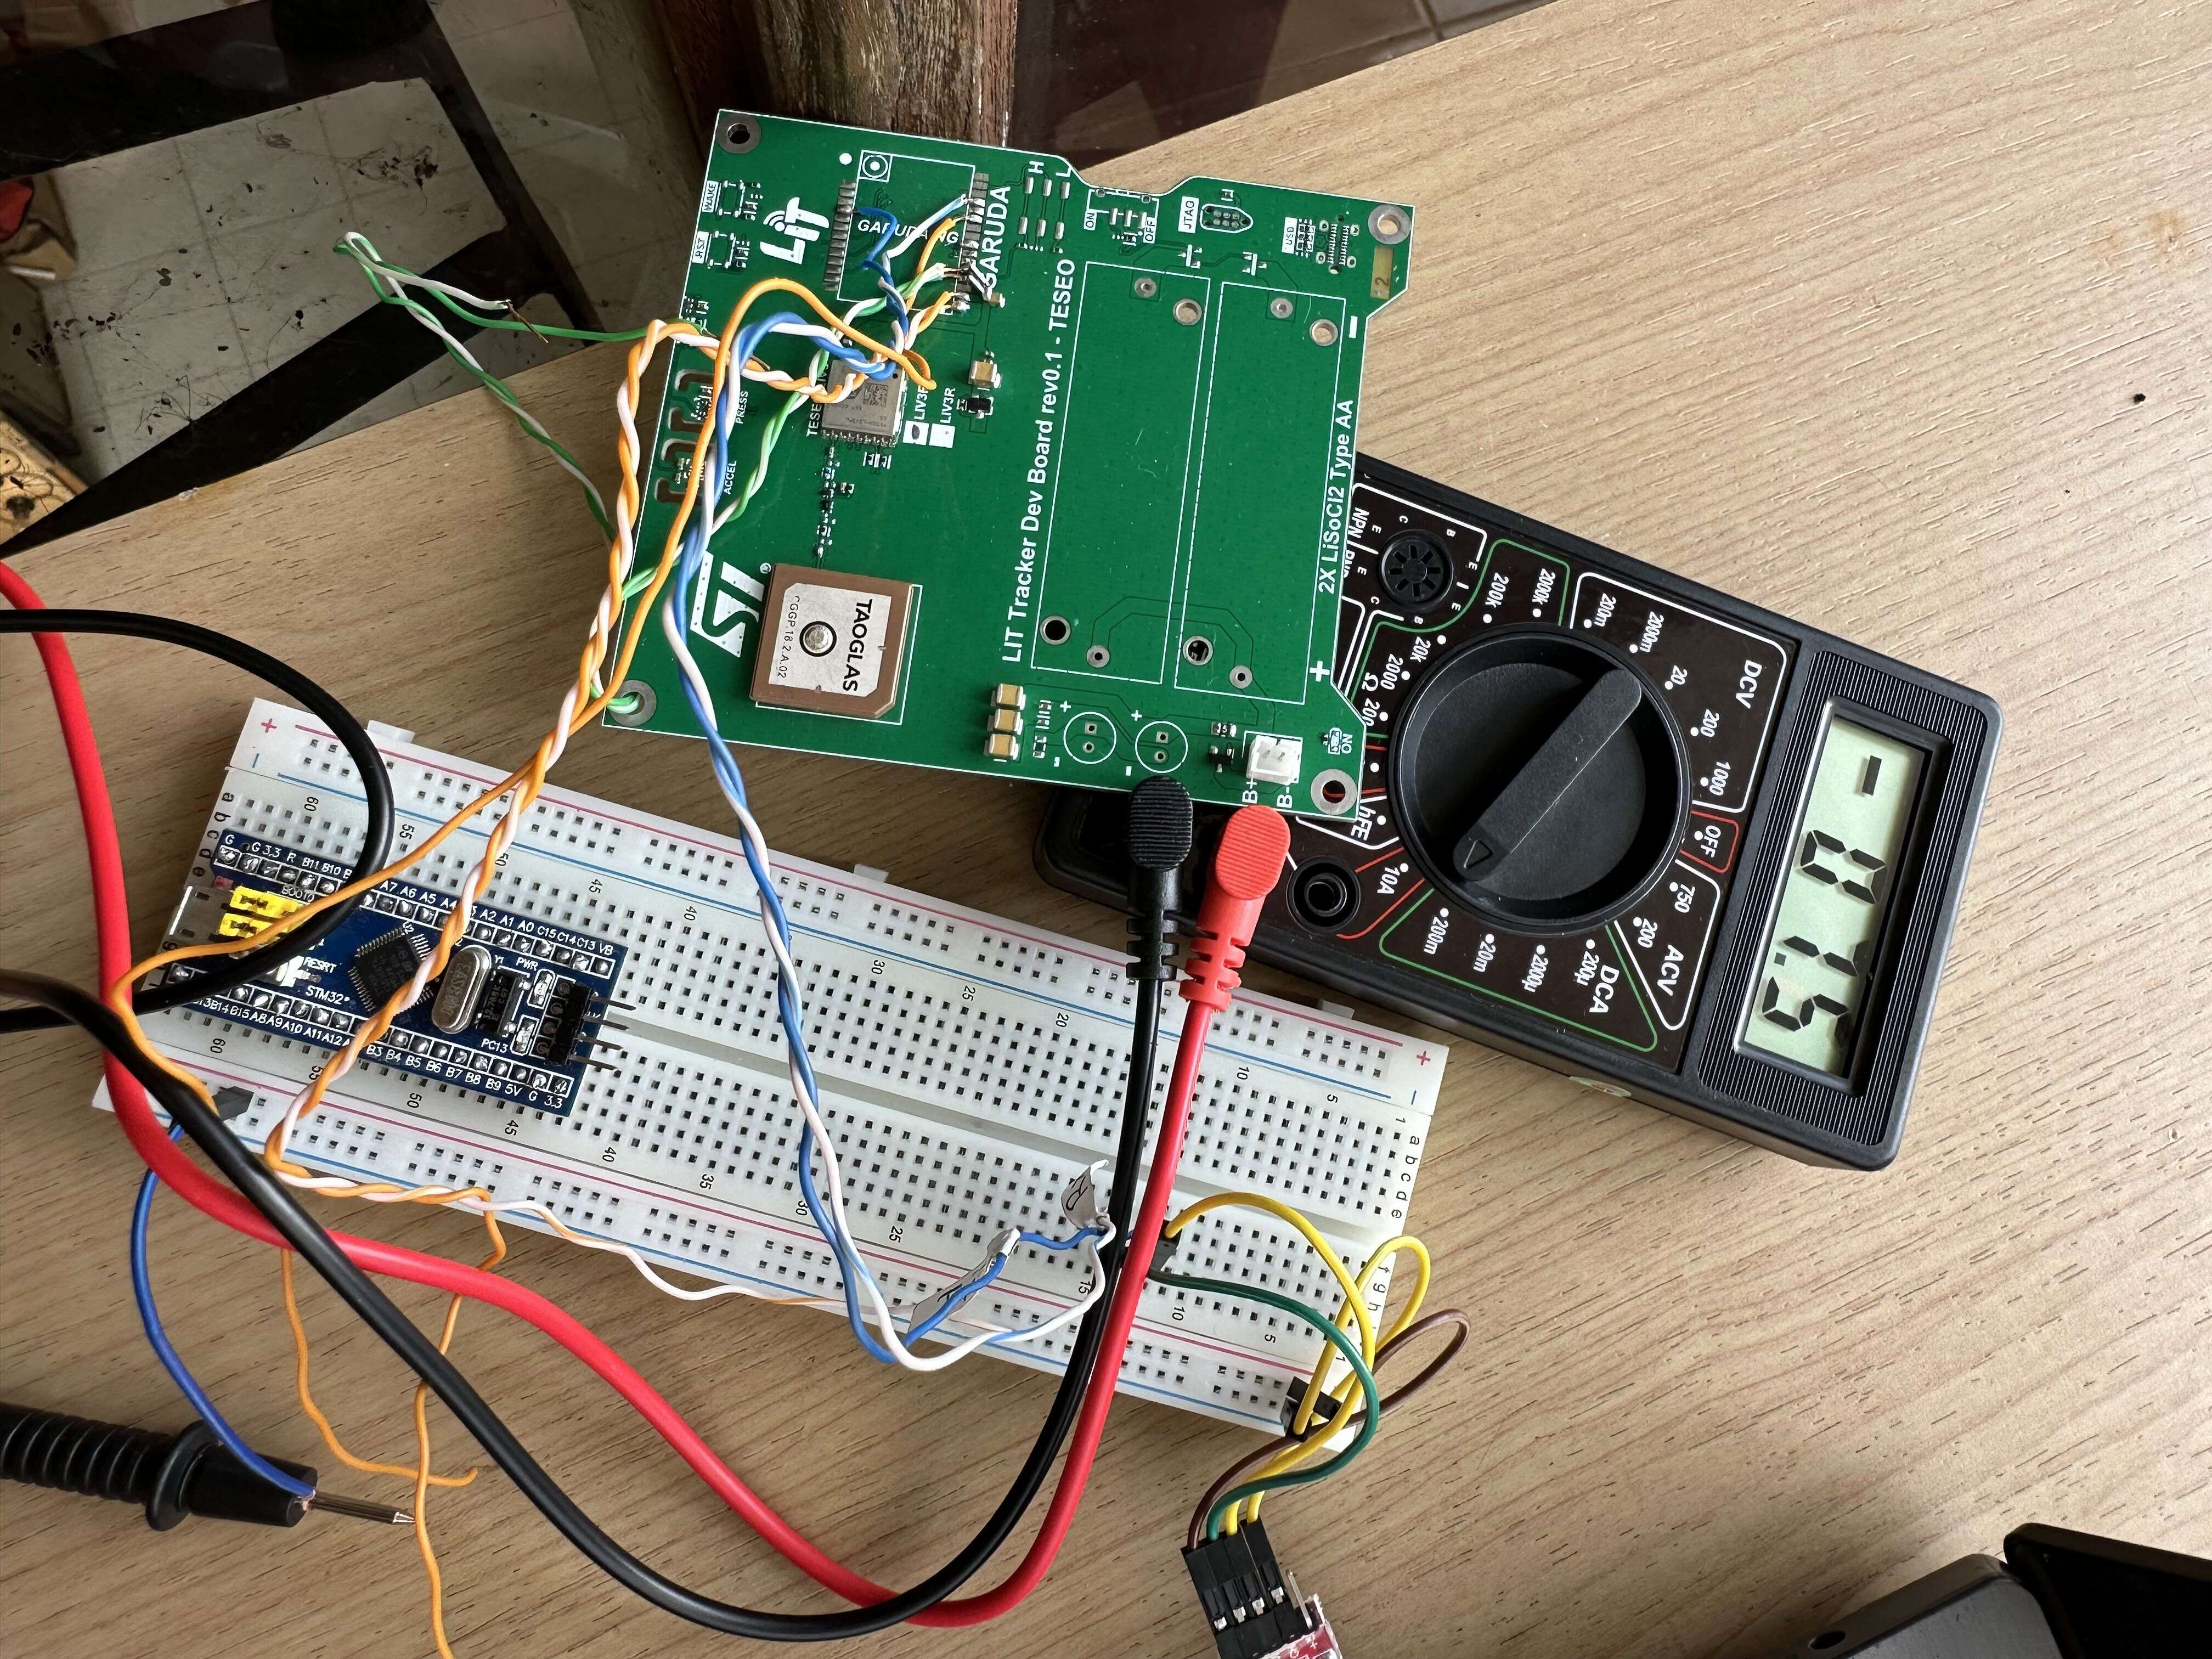
\includegraphics[width=10cm]{contents/chapter-4/low-power.jpg}
	\caption{Modul GNSS yang telah terangkai dengan multimeter}
	\label{Fig: low-power-connected}
\end{figure}

\section{Pengujian Mode Daya Rendah}
Pada pengujian daya rendah, konfigurasi \textit{common ground} digunakan saat merangkai modul Teseo\hyp{}LIV3FL dan multimeter agar keduanya dapat berbagi titik acuan yang sama. Hal ini memungkinkan pengukuran yang lebih akurat terhadap arus yang mengalir pada modul Teseo\hyp{}LIV3FL. Untuk menghubungkan modul Teseo\hyp{}LIV3FL dengan komputer, digunakan perangkat USB \textit{to} TTL \textit{converter} yang juga berfungsi sebagai sumber arus untuk menyalakan modul Teseo\hyp{}LIV3FL. Gambar \ref{Fig: low-power-connected} menunjukkan contoh dari modul Teseo\hyp{}LIV3FL yang sudah terhubung dengan multimeter dan siap untuk dilakukan pengujian daya rendah.

Algoritma daya rendah yang digunakan pada pengujian ini adalah mode periodik. Mode periodik pada modul Teseo\hyp{}LIV3FL memungkinkan modul tersebut berada dalam mode akuisisi dalam waktu tertentu hingga mendapatkan posisi fiksasi. Setelah modul Teseo\hyp{}LIV3FL mendapatkan posisi fiksasi, maka modul tersebut akan beralih ke mode \textit{standby} untuk menghemat daya. Kemudian, setelah periode waktu tertentu, modul Teseo\hyp{}LIV3FL akan kembali masuk ke mode akuisisi untuk mendapatkan posisi fiksasi kembali. Jika modul Teseo\hyp{}LIV3FL tidak dapat mendapatkan posisi fiksasi, maka modul tersebut akan tetap masuk ke mode \textit{standby} dan mencoba untuk mendapatkan posisi fiksasi kembali setelah periode waktu tertentu. Algoritma daya rendah ini sangat penting dalam memastikan modul Teseo\hyp{}LIV3FL mampu beroperasi dengan menggunakan daya yang sangat kecil namun tetap dapat mendapatkan posisi fiksasi dengan akurasi yang cukup baik.

Perintah \$PSTMLOWPOWERONOFF digunakan untuk mengendalikan mode daya rendah pada modul Teseo\hyp{}LIV3FL. Perintah ini menerima empat belas argumen dengan rincian tertentu untuk setiap mode daya rendah yang diaktifkan. Pada mode adaptif, empat argumen kedua hingga kelima digunakan untuk mengatur ambang batas untuk mode daya rendah, sedangkan pada mode \textit{cyclic}, digunakan dua argumen selanjutnya. Pada mode periodik, delapan argumen terakhir digunakan untuk mengatur frekuensi dan waktu mode daya rendah. Pada pengujian ini, digunakan mode daya rendah periodiksehingga argumen kedua hingga ketujuh harus diisi dengan angka nol. Perintah yang dikirimkan pada pengujian ini adalah \texttt{\$PSTMLOWPOWERONOFF,1,0,0,0,0,0,0,3,60,1,1,1,60,30}.

\begin{longtblr}[caption = {Argumen pada Perintah \$PSTMLOWPOWERONOFF}]{
	width = \linewidth,
	colspec = {Q[285]Q[48]Q[608]},
	row{1} = {c},
	row{3} = {c},
	row{5} = {c},
	row{6} = {c},
	row{7} = {c},
	row{8} = {c},
	row{10} = {c},
	row{11} = {c},
	cell{2}{1} = {c},
	cell{2}{2} = {c},
	cell{3}{1} = {c=3}{0.941\linewidth},
	cell{4}{1} = {c},
	cell{4}{2} = {c},
	cell{4}{3} = {r=4}{},
	cell{8}{1} = {c=3}{0.941\linewidth},
	cell{9}{1} = {c},
	cell{9}{2} = {c},
	cell{9}{3} = {r=2}{},
	cell{11}{1} = {c=3}{0.941\linewidth},
	cell{12}{1} = {c},
	cell{12}{2} = {c},
	cell{13}{1} = {c},
	cell{13}{2} = {c},
	cell{14}{1} = {c},
	cell{14}{2} = {c},
	cell{15}{1} = {c},
	cell{15}{2} = {c},
	cell{16}{1} = {c},
	cell{16}{2} = {c},
	cell{17}{1} = {c},
	cell{17}{2} = {c},
	cell{18}{1} = {c},
	cell{18}{2} = {c},
	hline{1-4,8-9,11-12} = {-}{},
}
\textbf{Argumen}                               & \textbf{Nilai} & \textbf{Keterangan}                                                                                                                      \\
Menyalakan atau mematikan mode daya rendah     & 1              & Mode daya rendah dinyalakan                                                                                                              \\
Mode Adaptif                                   &               0 &                                                                                                                                          \\
\textit{Constellation mask}                    & 0              & Mode adaptif tidak digunakan.                                                                                                            \\
Batas EHPE                            &               0 &                                                                                                                                          \\
Satelit maksimum                               &               0 &                                                                                                                                          \\
Perpindahan konstelasi otomatis                &         0       &                                                                                                                                          \\
Mode \textit{cyclic}                           &           0     &                                                                                                                                          \\
Menyalakan atau mematikan \textit{duty cycle} & 0              & Mode \textit{cyclic} tidak digunakan.\\
Periode \textit{duty cycle}                    &         0       &                                                                                                                                          \\
Mode periodik                                  &                &                                                                                                                                          \\
Mode periodik                                  & 3              & Mode periodik \textit{standby}                                                                                                          \\
FixPeriod                                      & 60             & Modul akan memasuki mode~\textit{standby} selama enam puluh detik setelah mendapat posisi fiksasi                                \\
FixOnTime                                      & 3              & Memasuki mode \textit{standby} setelah mendapatkan tiga posisi fiksasi                                                           \\
Penyegaran ephemeris                           & 1              & Penyegaran ephemeris diaktifkan                                                                                                          \\
Kalibrasi RTC                                  & 1              & Kalibrasi RTC diaktifkan                                                                                                                 \\
NoFixCnt                                       & 60             & Modul akan memasuki mode \textit{standby} jika tidak bisa mendapatkan posisi \textit{fix~setelah enam puluh detik (\textit{fix loss)}} \\
NoFixOff                                       & 30             & Modul memasuki \textit{standby} selama tiga puluh detik setelah \textit{fix loss}\\
\hline                                                      
\end{longtblr}

Perintah tersebut akan mengaktifkan mode daya rendah periodik pada modul Teseo\hyp{}LIV3FL dengan waktu \textit{standby} selama satu menit setelah mendapatkan tiga posisi fiksasi. Artinya, setelah modul menerima tiga posisi fiksasi, maka modul akan masuk ke mode daya rendah dan hanya akan mengambil posisi setiap satu menit. Selain itu, modul juga akan menuju mode \textit{standby} selama tiga puluh detik jika tidak dapat mendapatkan posisi fiksasi selama satu menit. Detail argumen yang digunakan pada pengujian ini dapat dilihat pada Tabel 4.1.

\begin{figure}[H]
	\centering
	\captionsetup{justification=centering}
	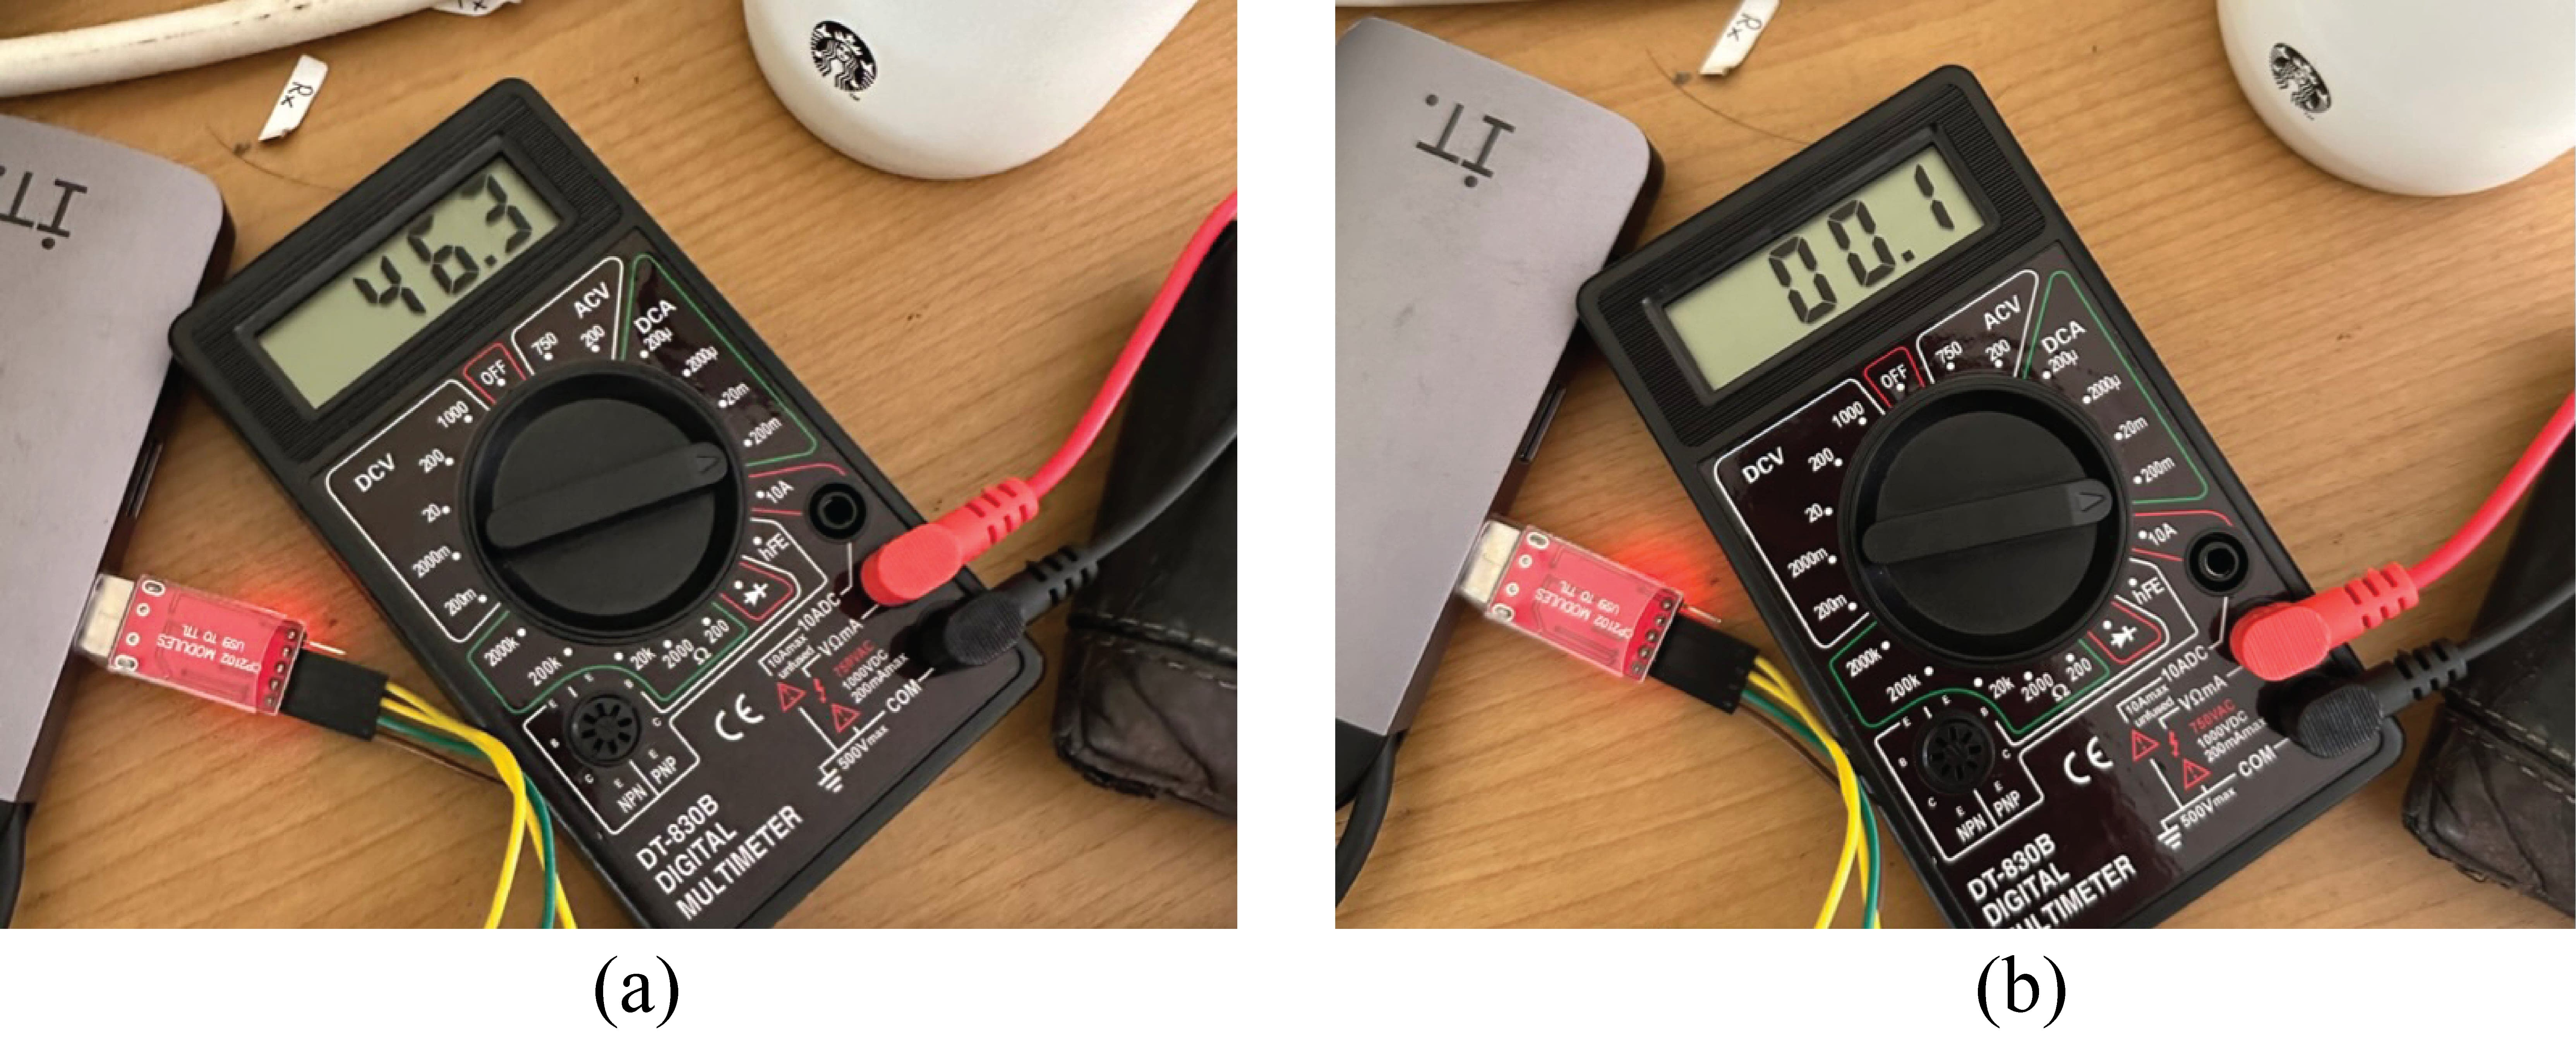
\includegraphics[width=14cm]{contents/chapter-4/low-power-result.jpg}
	\caption{Pembacaan multimeter pada. (a) Mode akuisisi. (b) Mode \textit{standby}}
	\label{Fig: low-power-result}
\end{figure}

Hasil pengukuran menunjukkan bahwa arus yang mengalir pada modul Teseo\hyp{}LIV3FL adalah sebesar 46,3 mA. Namun, hal yang menarik adalah nilai arus yang diukur jauh lebih kecil daripada nilai arus yang tertera pada \textit{datasheet}, yang mencapai 65 mA. Dalam mode akuisisi, modul Teseo\hyp{}LIV3FL berada dalam kondisi siap dan hanya menunggu untuk melakukan pencarian posisi kembali. Oleh karena itu, arus yang mengalir pada modul Teseo\hyp{}LIV3FL sudah sama dengan nilai \textit{datasheet}, yaitu sebesar 10 $\mu$A. Hal ini menunjukkan bahwa penggunaan mode daya rendah pada modul Teseo\hyp{}LIV3FL dapat menurunkan konsumsi daya yang ditunjukan dengan penurunan jumlah arus ketika berada dalam mode \textit{standby}. Gambar \ref{Fig: low-power-result}a menunjukkan hasil pengukuran multimeter ketika modul Teseo\hyp{}LIV3FL berada dalam mode akuisisi dan Gambar \ref{Fig: low-power-result}b untuk mode daya rendah (kanan). Hasil yang didapat menunjukkan perbedaan yang signifikan dalam tingkat konsumsi daya antara kedua mode tersebut.

\begin{table}[H]
	\caption{Performa Modul GNSS dengan Variasi Waktu \textit{Standby}}
	\vspace{0.5em}
	\centering
	\begin{tabular}{ccccc}
		\hline
		\textbf{Waktu \textit{Standby}} &\textbf{TTFF (s)} & \textbf{HDOP} & \textbf{Visibilitas Satelit} & \textbf{Fiksasi}\\
		\hline 
		1 menit & 8,47 & 1,5 & 9 & 3D\\
		2 menit & 11,24 & 1,1 & 8 & 3D\\
		3 menit & 11,47 & 1,8 & 8 & 3D\\
		4 menit & 19,46 & 2,6 & 5 & 2D\\
		5 menit & 20,65 & 3,5 & 5 & 2D\\
		6 menit & $\infty$ & - & - & -\\
		\hline
	\end{tabular}
	\label{Tab: standby-time-test}
\end{table}

Selain arus yang mengalir pada modul, performa dari modul Teseo\hyp{}LIV3FL juga perlu diuji lebih lanjut. Tabel \ref{Tab: standby-time-test} menunjukan performa GNSS dengan berbagai skenario waktu \textit{standby} setelah mendapat fiksasi. Terlihat bahwa jika waktu \textit{standby} semakin lama maka waktu untuk mendapatkan fiksasi pertama (TTFF) juga semakin lama. Ketika waktu \textit{standby} diatur lebih dari 3 menit, fiksasi yang didapat hanyalah 2D. Jika waktu mode \textit{standby} diatur menjadi 6 menit atau lebih, modul Teseo\hyp{}LIV3FL akan semakin sulit untuk mengunci satelit dan mendapatkan fiksasi.

Ketika modul GNSS berada di mode \textit{standby} dalam waktu yang lama, data efemeris yang dimiliki akan menjadi usang. Hal tersebut menyebabkan modul harus mencari data efemeris kembali. Selain itu, modul GNSS juga bekerja dengan prinsip \textit{line-of-sight}. Ketika modul GNSS kembali ke keadaan akuisisi setelah \textit{standby}, \textit{line-of-sight} pada waktu tersebut sudah berbeda dari waktu ketika modul GNSS tepat masuk ke mode \textit{standby}.

\section{Pengujian \textit{Rapid Static Survey}}
Rapid Static Survey adalah pengujian yang dilakukan untuk meninjau performa modul GNSS dalam keadaan diam. Pengujian ini dapat dilakukan dalam rentang waktu 15 menit sampai dengan 2 jam \cite{lauer2019static}. Pengujian ini akan meninjau  dan presisi dari modul GNSS. Akurasi adalah tingkat kedekatan hasil pembacaan modul GNSS dengan posisi sebenarnya, sedangkan tingkat presisi menunjukan seberapa dekat hasil yang didapat dengan rata-rata dari seluruh sampel \cite{gnssca_apn029}.

Pada pengujian \textit{rapid static survey}, modul Teseo\hyp{}LIV3FL diletakan dalam empat skenario selama satu jam. Skenario tersebut meliputi \textit{basement}, dalam ruangan, ruangan semi terbuka, dan ruang terbuka. Pengujian setiap skenario dilakukan pada empat titik di lingkungan Universitas Gadjah Mada, yaitu:

\begin{enumerate}
	\item \textit{Basement} diwakili oleh tempat parkir bawah tanah milik Fakultas Ilmu Sosial dan Ilmu Politik.
	\item Ruangan tertutup diwakili oleh Lantai 5 Gedung SGLC Fakultas Teknik.
	\item Ruang semi terbuka diwakili oleh Selasar Grha Sabha Pramana.
	\item Ruangan terbuka diwakili oleh Lapangan Pancasila.
\end{enumerate}

Nilai HDOP (\textit{Horizontal Dilution of Precision}), VDOP (\textit{Vertical Dilution of Precision}), PDOP (\textit{Position Dilution of Precision}), \textit{Circular Error Probability} (CEP), dan MAD (\textit{Mean Absolute Deviation}) adalah parameter yang digunakan untuk mengevaluasi akurasi dan presisi dari pengukuran GNSS. Pada pengujian Rapid Static Survey, nilai-nilai HDOP, VDOP, PDOP, CEP, dan MAD akan diamati di setiap skenario pengujian. Hal ini akan memberikan informasi tentang seberapa akurat dan presisi posisi yang dihasilkan oleh modul Teseo\hyp{}LIV3FL dalam berbagai kondisi lingkungan dan dapat membantu dalam mengevaluasi performa modul GNSS.

\begin{figure}[H]
	\centering
	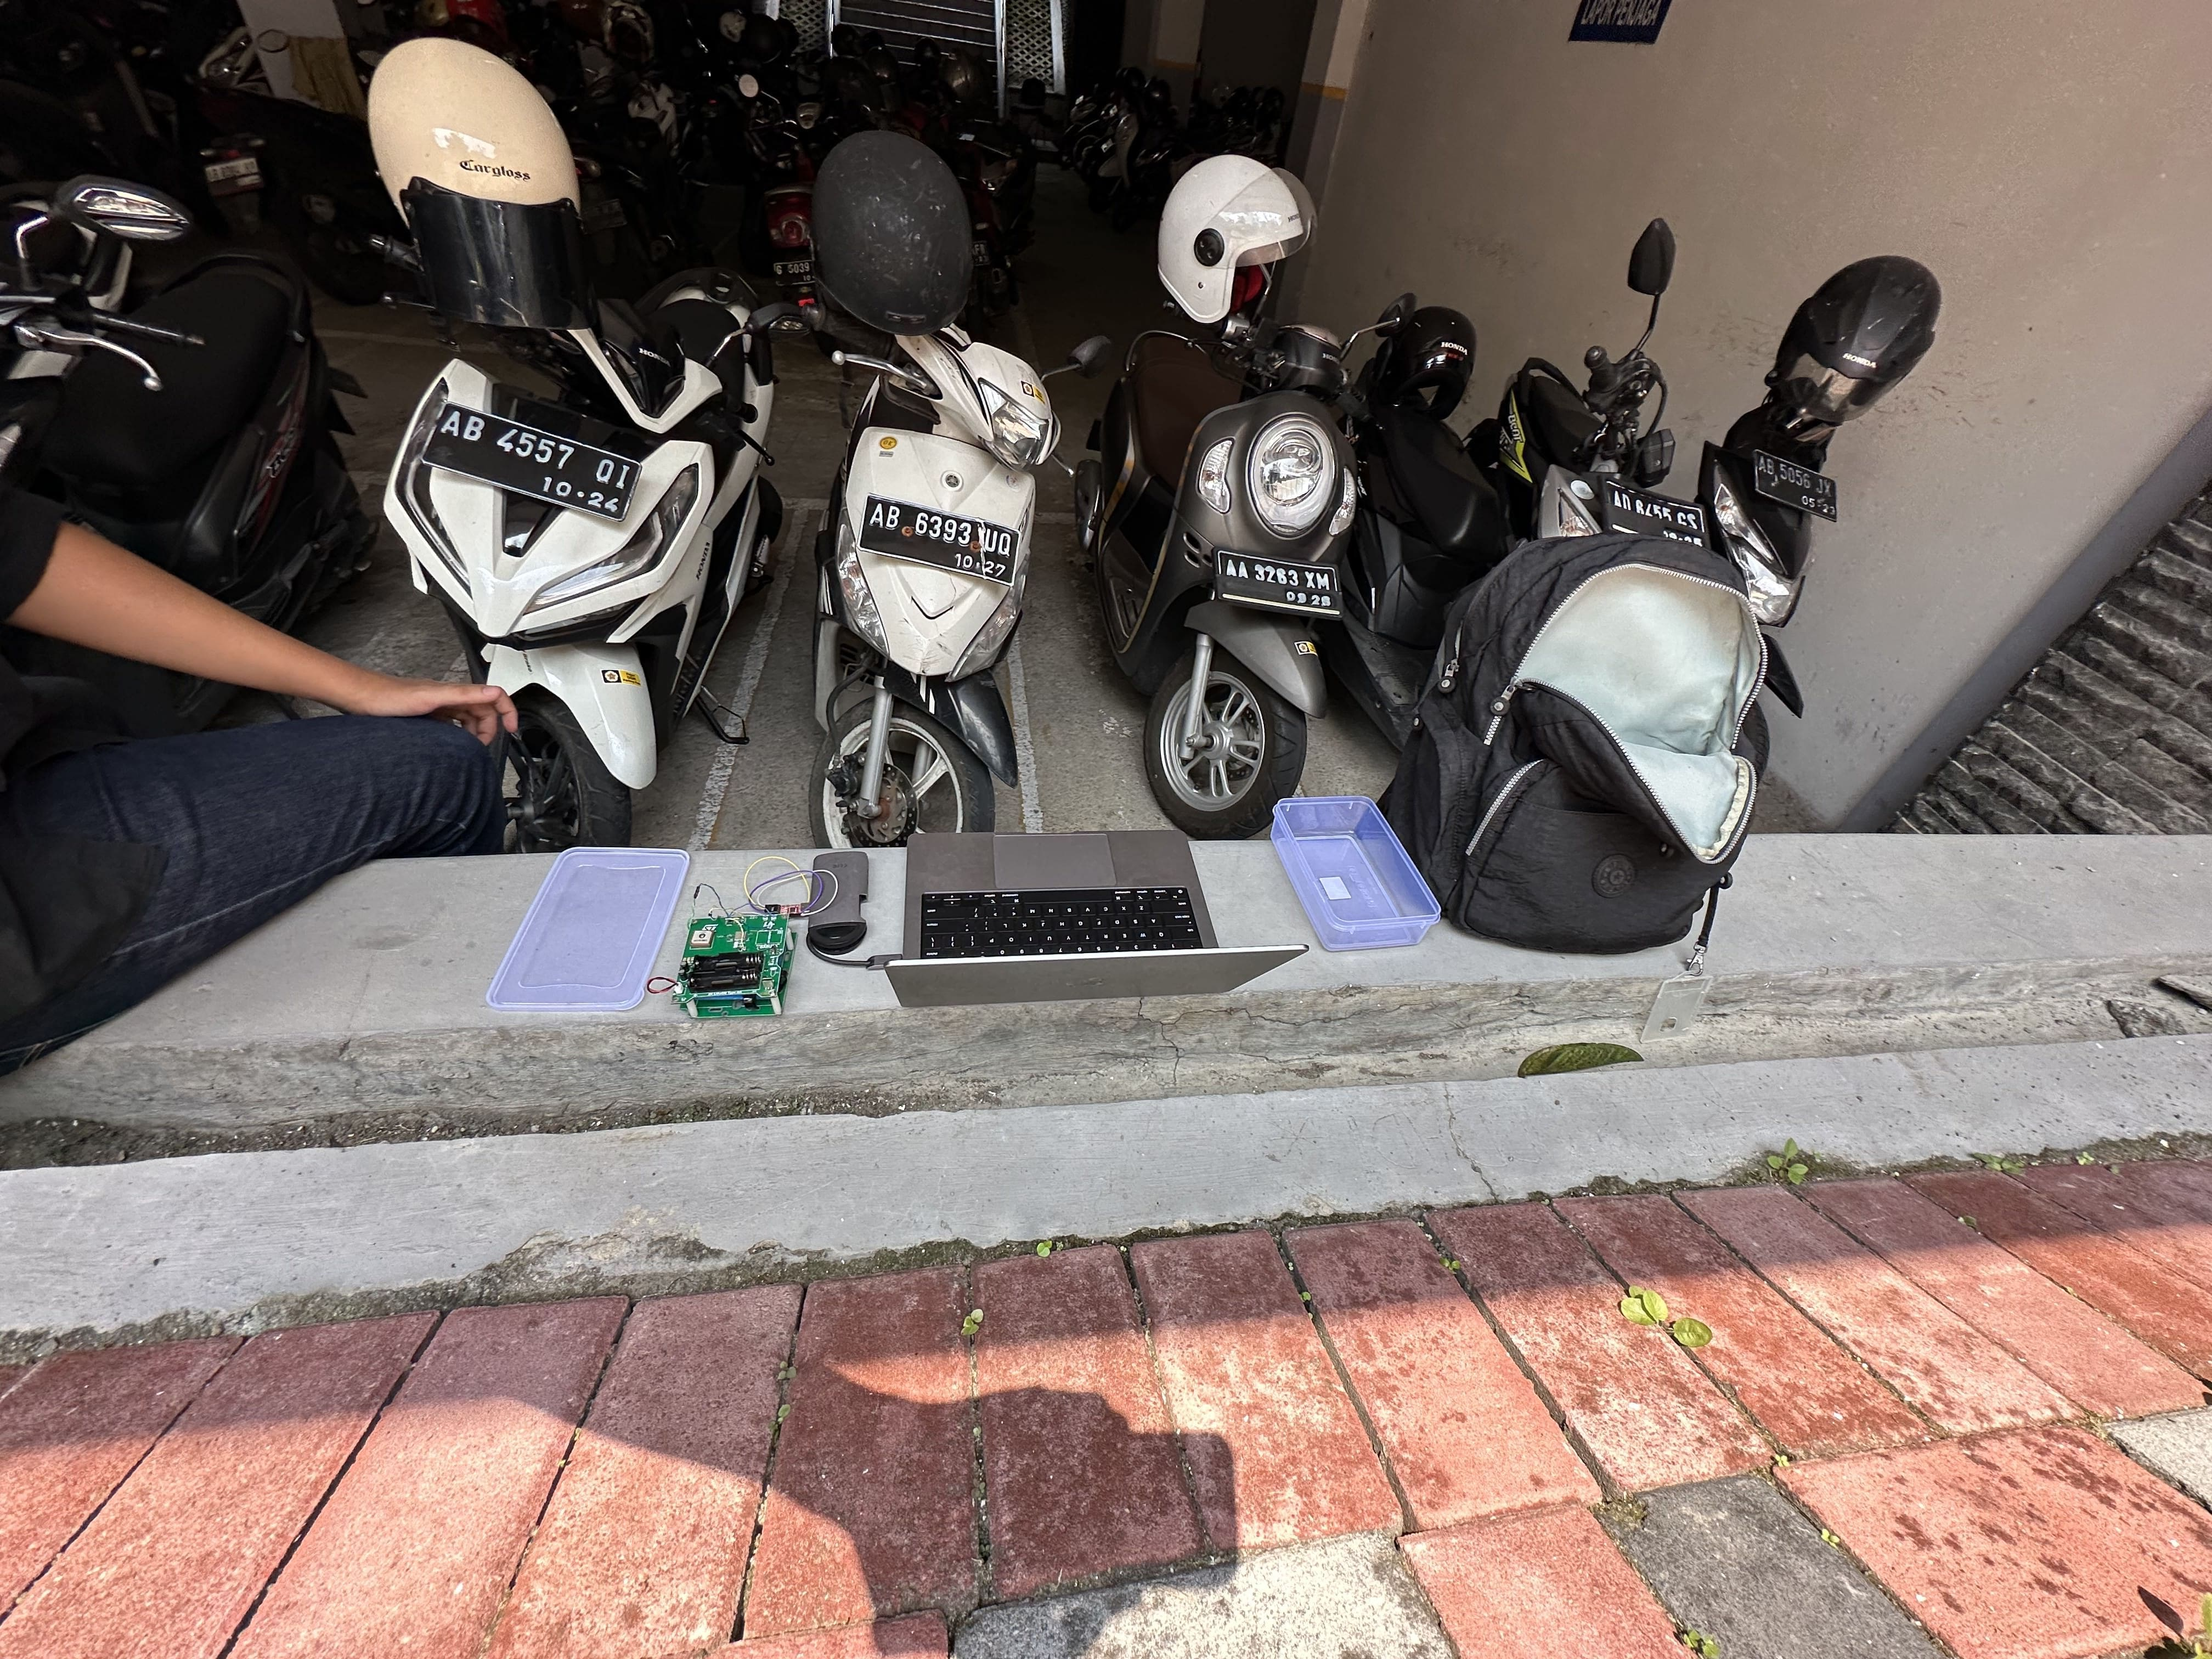
\includegraphics[width=10cm]{contents/chapter-4/1-skenario-basement/keadaan.jpg}
	\caption{Keadaan sekitar pengujian skenario \textit{basement}}
	\label{Fig: basement-keadaan}
\end{figure}

\subsection{Skenario \textit{Basement}}
Pengujian skenario \textit{basement} dilakukan dengan tujuan untuk memperoleh gambaran tentang performa modul Teseo\hyp{}LIV3FL di dalam ruangan bawah tanah. Ruangan bawah tanah seringkali digunakan sebagai tempat parkir mobil, gudang, atau ruang penyimpanan yang berada di bawah gedung. Karena letaknya yang berada di bawah tanah, maka akses isyarat satelit GNSS menjadi terbatas.

\begin{figure}[H]
	\centering
	\begin{adjustbox}{width=\textwidth}
		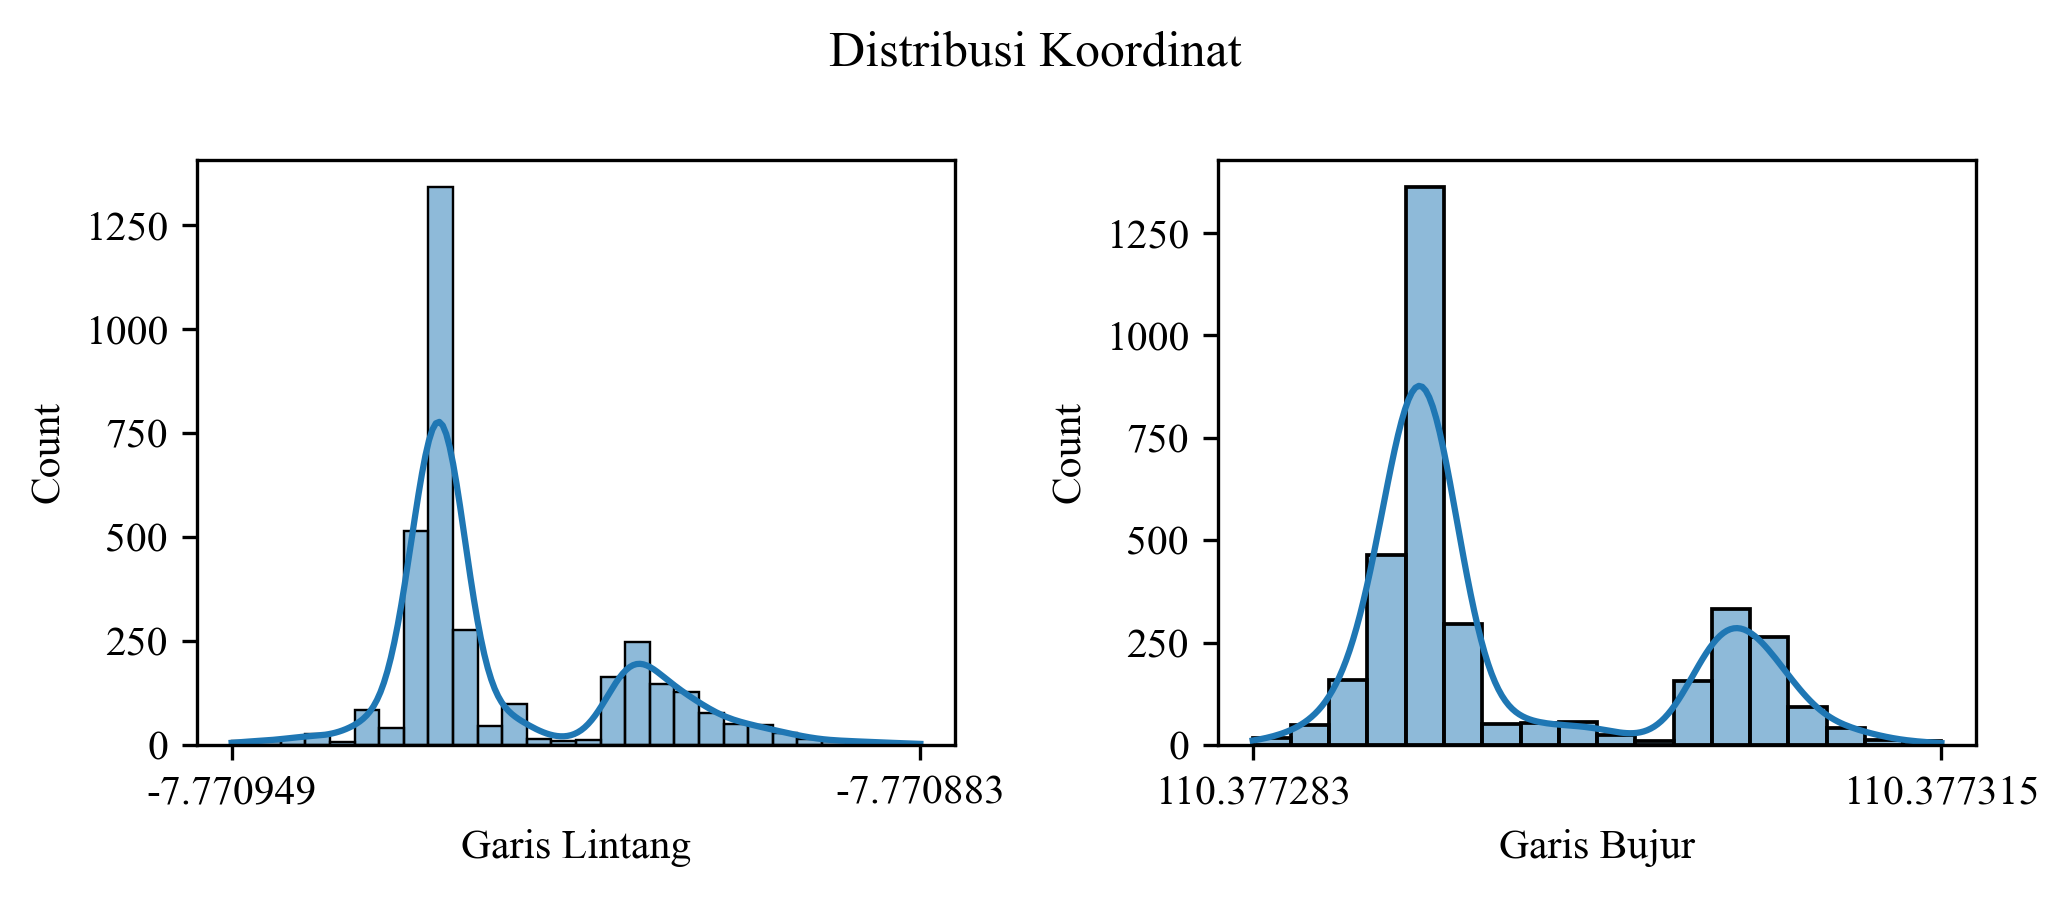
\includegraphics{contents/chapter-4/1-skenario-basement/distribution.png}
	\end{adjustbox}
	\caption{Distribusi data koordinat skenario \textit{basement}}
	\label{Fig:basement-distribution}
\end{figure}

Dalam pengujian ini, modul Teseo\hyp{}LIV3FL diletakkan di tempat parkir bawah tanah yang berada di bawah gedung empat lantai dengan struktur beton. Pengujian dilakukan pada lingkungan yang sangat tertutup dan minim sinar matahari. Terdapat beberapa area terbuka kecil yang memungkinkan sedikit sinar matahari untuk masuk. Gambar \ref{Fig: basement-keadaan} menunjukkan kondisi lingkungan saat pengujian skenario \textit{basement}.

\begin{figure}[H]
	\centering
	\includegraphics[width=10cm]{contents/chapter-4/1-skenario-basement/sky_plot.png}
	\caption{\textit{Sky plot} pengujian skenario \textit{basement}}
	\label{Fig: basement-skyplot}
\end{figure}

\begin{table}[H]
	\caption{Hasil Pengujian Skenario \textit{Basement}}
	\vspace{0.5em}
	\centering
	\begin{tabular}{ccccc}
		\hline
		& \textbf{Minima} & \textbf{Maxima} & \textbf{Rata-rata} & \textbf{Standar Deviasi}\\
		\hline 
		HDOP & 1,80 & 26,80 & 6,67 & 5,03\\
		VDOP & 2,00 & 28,80 & 8,27 & 5,36\\
		PDOP & 2,80 & 39,30 & 10,67 & 7,30\\
		CEP (m) & 11,65 & 79,56 & 32,69 & 13,34\\
		Visibilitas Satelit & 5 & 12 & 7,60 & 1,27\\
		\hline
		\textbf{MAD-x (m)} & & \multicolumn{2}{c}{\centering 18,89} & \\
		\hline
		\textbf{MAD-y (m)} & & \multicolumn{2}{c}{\centering 14,99} & \\
		\hline
		\textbf{MAD (m)} & & \multicolumn{2}{c}{\centering 24,11} & \\
		\hline
	\end{tabular}
	\label{Tab: basement-table}
\end{table}

Grafik persebaran distribusi koordinat pada Gambar \ref{Fig:basement-distribution} menunjukkan bahwa koordinat garis lintang memiliki rentang tersebar antara -7,769728 hingga -7,768525 sedangkan untuk garis bujur memiliki rentang tersebar antara 110,379841 hingga 110,380314. Terlihat bahwa kedua koordinat tidak terdistribusi secara normal sehingga perlu dilakukan analisis statistik non-parametrik, yaitu MAD.

\begin{figure}[H]
	\centering
	\begin{adjustbox}{width=\textwidth}
		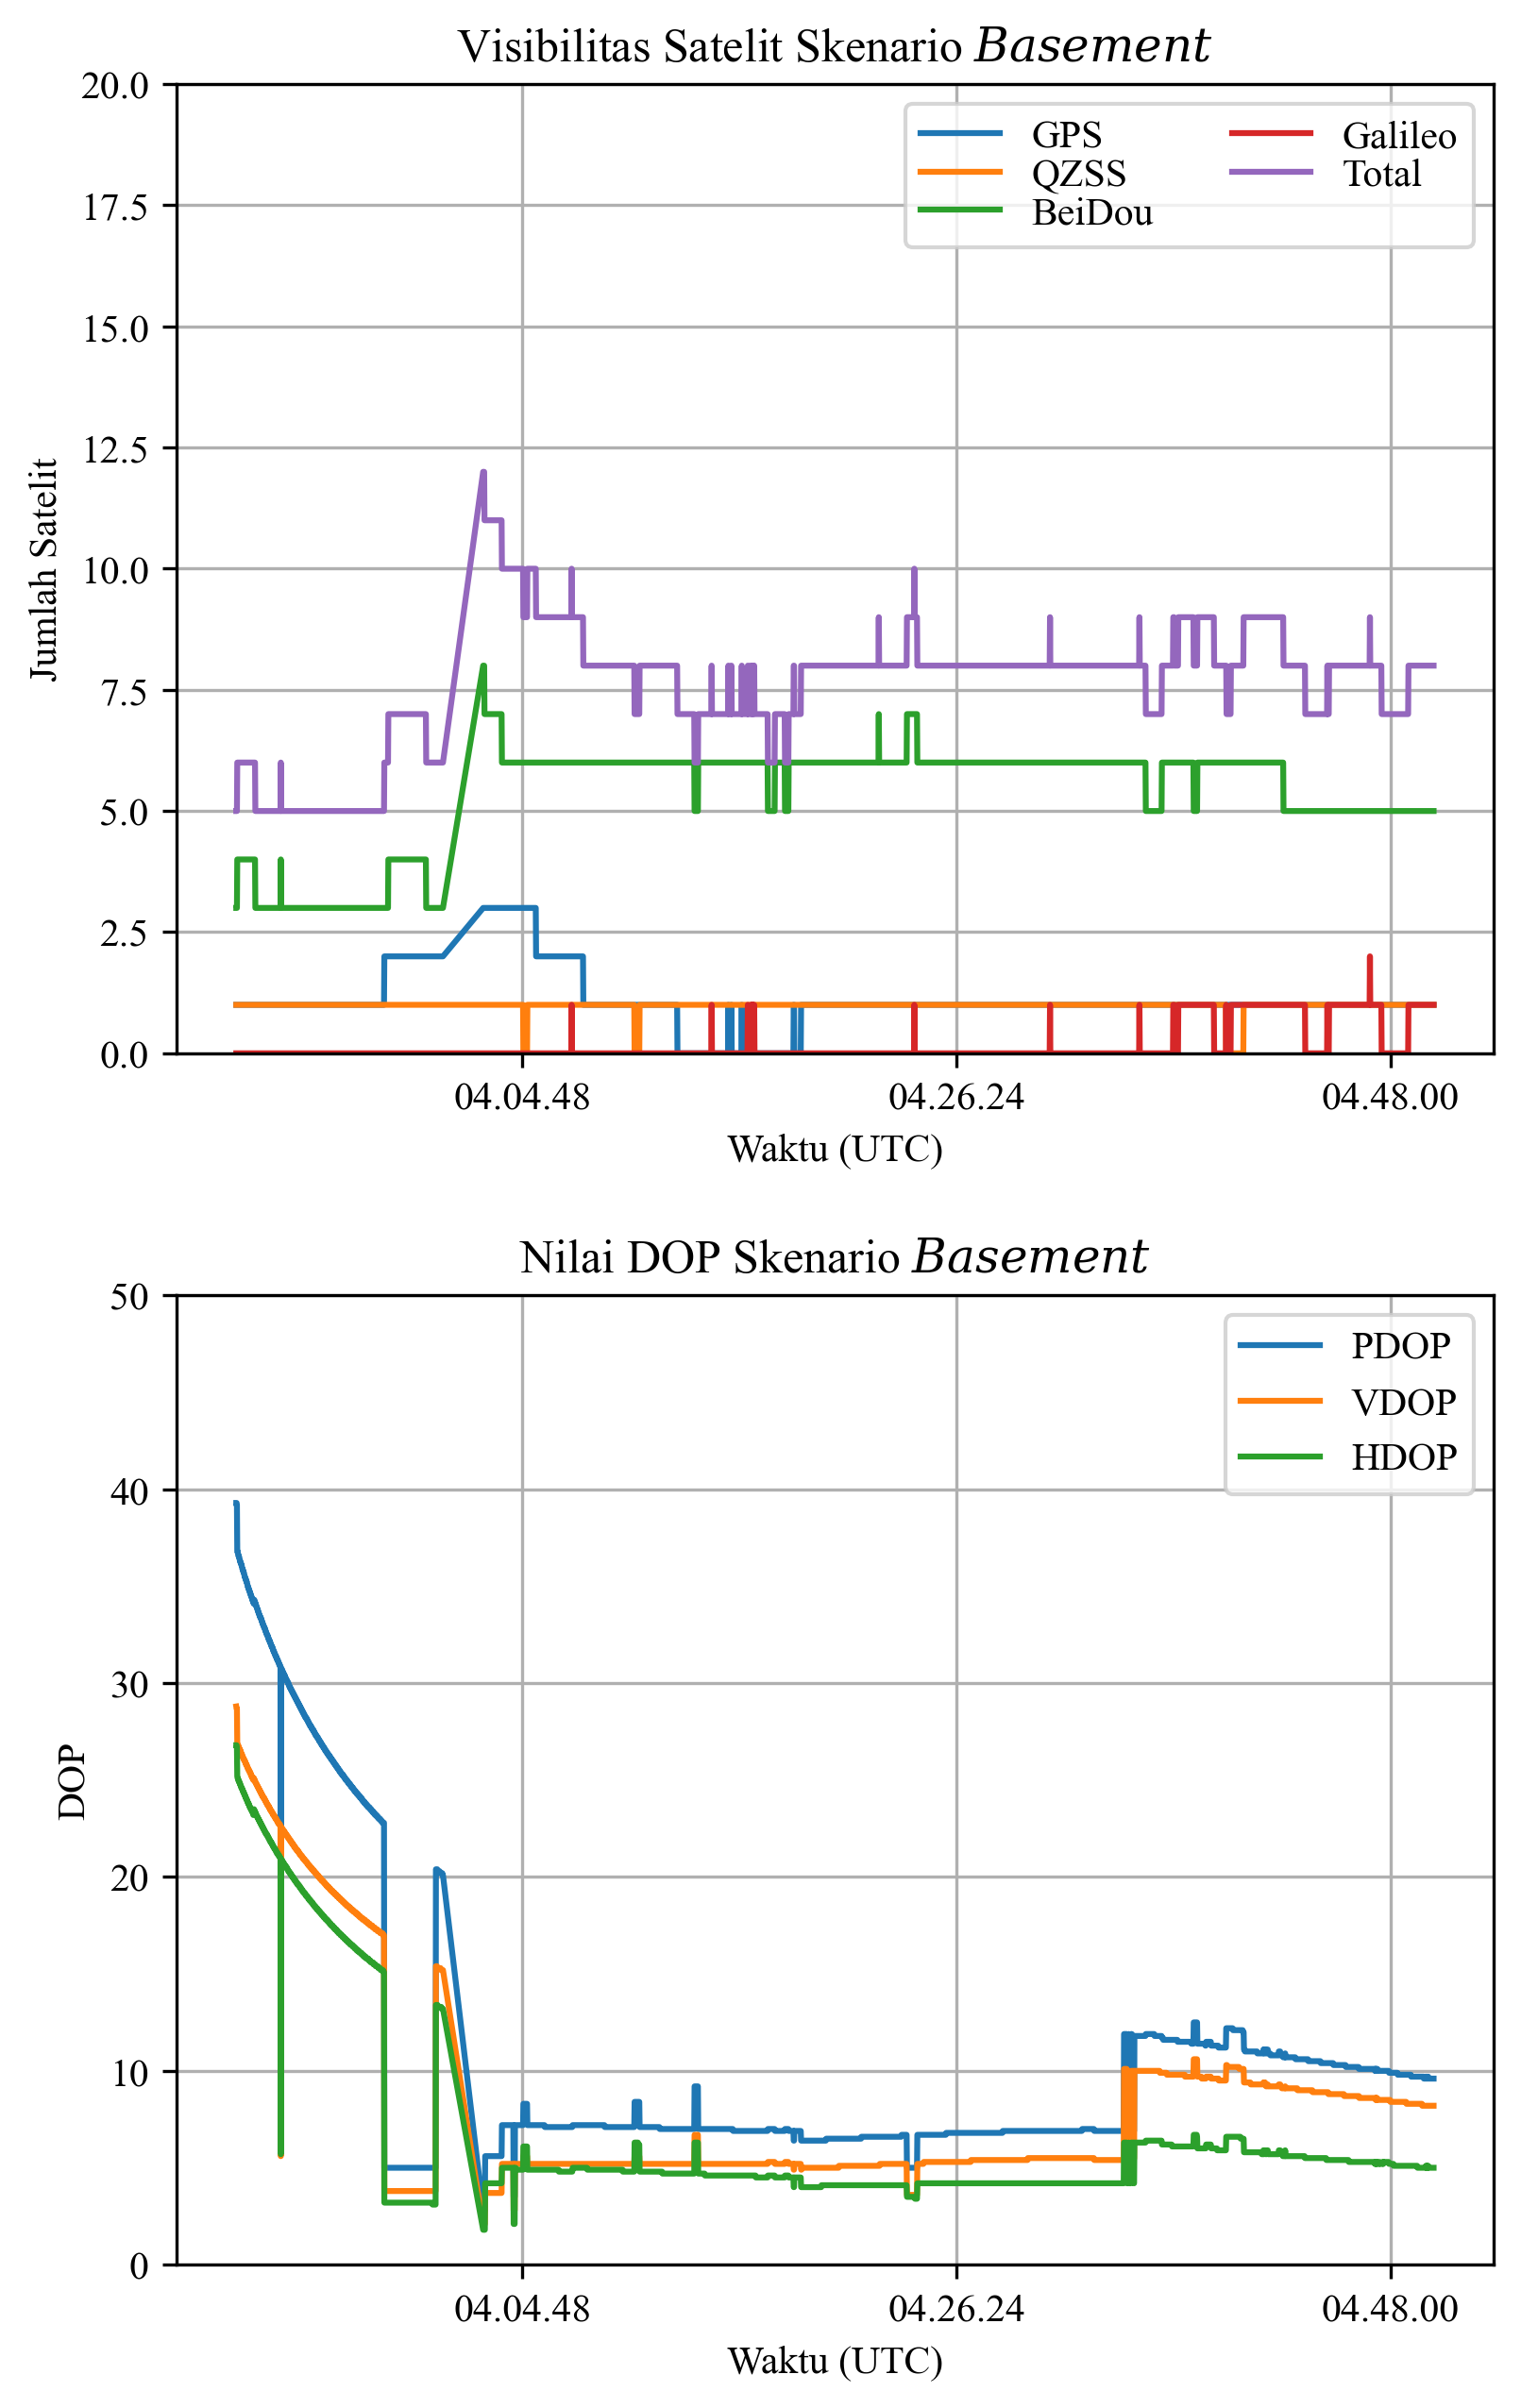
\includegraphics{contents/chapter-4/1-skenario-basement/sats_dop.png}
	\end{adjustbox}
	\caption{DOP dan visibilitas satelit pengujian skenario \textit{basement}}
	\label{Fig: basement-sats_dop}
\end{figure}

Pada skenario \textit{basement}, hasil pengukuran modul Teseo\hyp{}LIV3FL menunjukkan hasil yang kurang akurat. Hal ini terlihat pada data yang dicatat pada Gambar \ref{Fig: basement-sats_dop}, yang menunjukkan adanya lonjakan nilai DOP. Selain itu, nilai maksimum PDOP yang dicatat pada Tabel \ref{Tab: basement-table} adalah sebesar 39,30. Nilai yang sangat tinggi ini mengindikasikan bahwa persebaran satelit di langit tidak mencakup seluruh lingkaran, seperti terlihat pada \textit{sky plot} pada Gambar \ref{Fig: basement-skyplot}. \textit{Sky plot} tersebut memperlihatkan bahwa persebaran satelit hanya mencakup setengah bagian dari lingkaran sehingga dapat mempengaruhi akurasi keseluruhan dari hasil pengukuran modul Teseo\hyp{}LIV3FL. Analisis MAD menunjukan bahwa tingkat kepresisian modul Teseo-LIV3Fl pada skenario \textit{basement} adalah 18,89 meter pada sumbu garis lintang, 14,99 pada sumbu garis bujur, dan 24,11 meter secara keseluruhan.

\begin{figure}[H]
	\centering
	\includegraphics[width=13cm]{contents/chapter-4/1-skenario-basement/cep.png}
	\caption{CEP pengujian skenario \textit{basement}}
	\label{Fig: basement-cep}
\end{figure}

Selain MAD, tingkat presisi dari modul GNSS juga dapat ditinjau dengan menggunakan CEP atau \textit{Circular Error Probability}. Tren nilai CEP selama satu jam ditunjukan oleh Gambar \ref{Fig: basement-cep}. Dapat dilihat bahwa pada awal pengujian terjadi lonjakan nilai CEP hingga delapan puluh meter pada sepuluh hingga lima belas menit pertama. Hal tersebut sejalan dengan visibilitas satelit paling rendah yang juga terjadi pada rentang waktu tersebut. 

Seiring berjalannya waktu, visibilitas satelit mulai membaik dan nilai CEP juga ikut menurun. Rata-rata CEP pada pengujian ini adalah 32,69 meter dengan standar deviasi 13,34 meter. Nilai tersebut menunjukan bahwa data memiliki tingkat variasi yang cukup besar. Tingkat variasi yang cukup besar menunjukan bahwa data koordinat yang dimiliki cenderung lebih jauh dari rata-ratanya.

\begin{figure}[H]
	\centering
	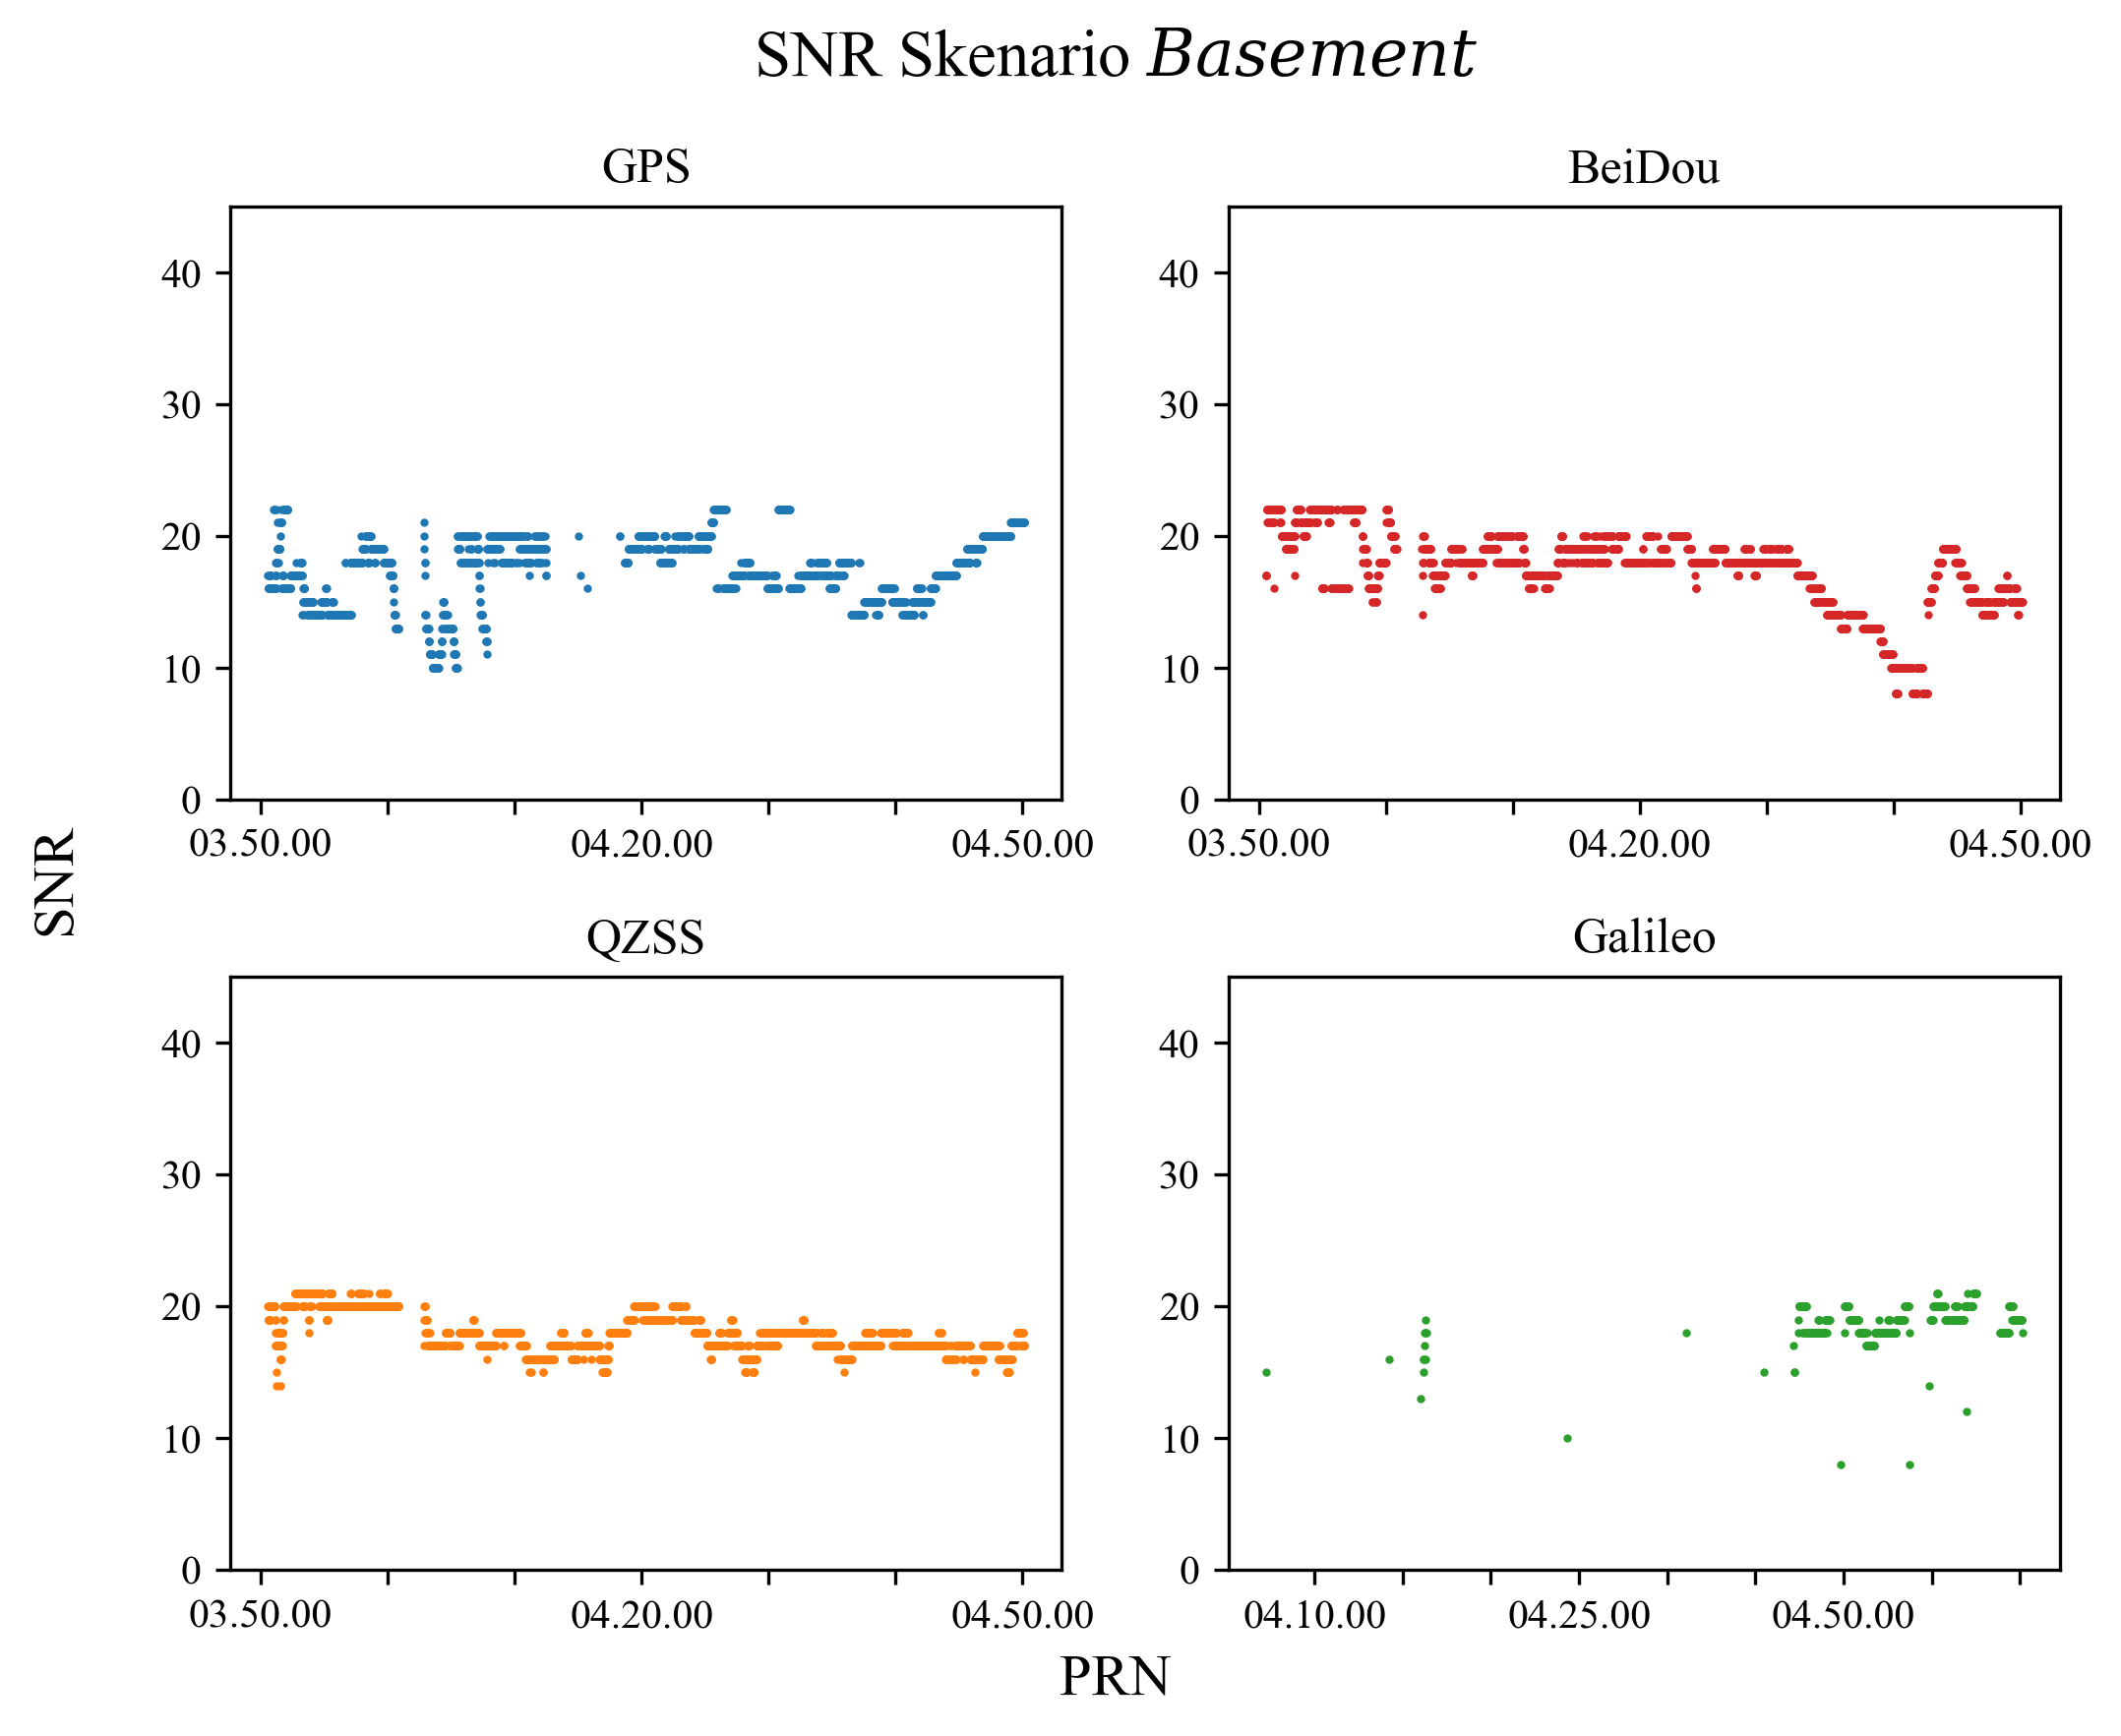
\includegraphics[width=13cm]{contents/chapter-4/1-skenario-basement/snr.png}
	\caption{SNR setiap konstelasi pada pengujian skenario ruang terbuka}
	\label{Fig: basement-snr}
\end{figure}

Jika dilihat dari nilai SNR pada Gambar \ref{Fig: basement-snr}, terlihat bahwa selain diakibatkan visibilitas satelit yang rendah, lonjakan nilai CEP pada 10 menit pertama pengamatan diakibatkan oleh nilai SNR pada konstelasi yang cenderung sangat rendah. Setelah SNR dari konstelasi membaik, nilai CEP juga ikut membaik. Bagian kosong pada konstelasi Galileo sejalan dengan visibilitas satelit dari konstelasi Galileo yang sangat rendah. Pada skenario ini, visibilitas satelit memiliki peran yang sangat penting untuk memperbaiki nilai CEP.

Meskipun modul Teseo\hyp{}LIV3FL tertutup oleh struktur beton, modul tetap mampu menangkap isyarat dari keempat konstelasi Teseo\hyp{}LIV3FL yang telah diatur. Dari hasil pengujian, terlihat bahwa konstelasi dengan jumlah satelit paling banyak adalah BeiDou milik Republik Rakyat Tiongkok. Namun, terjadi lonjakan nilai DOP pada awal pengujian saat jumlah satelit paling rendah. Hal ini menunjukkan bahwa jumlah satelit yang rendah akan meningkatkan ketiga nilai DOP, yang pada akhirnya akan menurunkan akurasi dari hasil pembacaan modul Teseo\hyp{}LIV3FL.

Angka 24,11 meter pada hasil analisis MAD menunjukan tingkat presisi masih rendah, tetapi nilai rata-rata HDOP yang menunjukan angka 8,27 tetap menunjukan bahwa hasil pengukuran posisi masih layak untuk digunakan. Perlu diingat bahwa pengujian ini dilakukan di lingkungan yang sangat sulit, yaitu ruangan bawah tanah dengan struktur beton yang menutupi sinyal dari satelit. Selain itu, terdapat sedikit bagian terbuka yang memungkinkan sinar matahari untuk memasuki ruangan. Meskipun demikian, pengujian ini menunjukan bahwa modul GNSS masih dapat digunakan untuk mendapatkan posisi fiksasi dalam kondisi lingkungan yang sulit.

\begin{figure}[H]
	\centering
	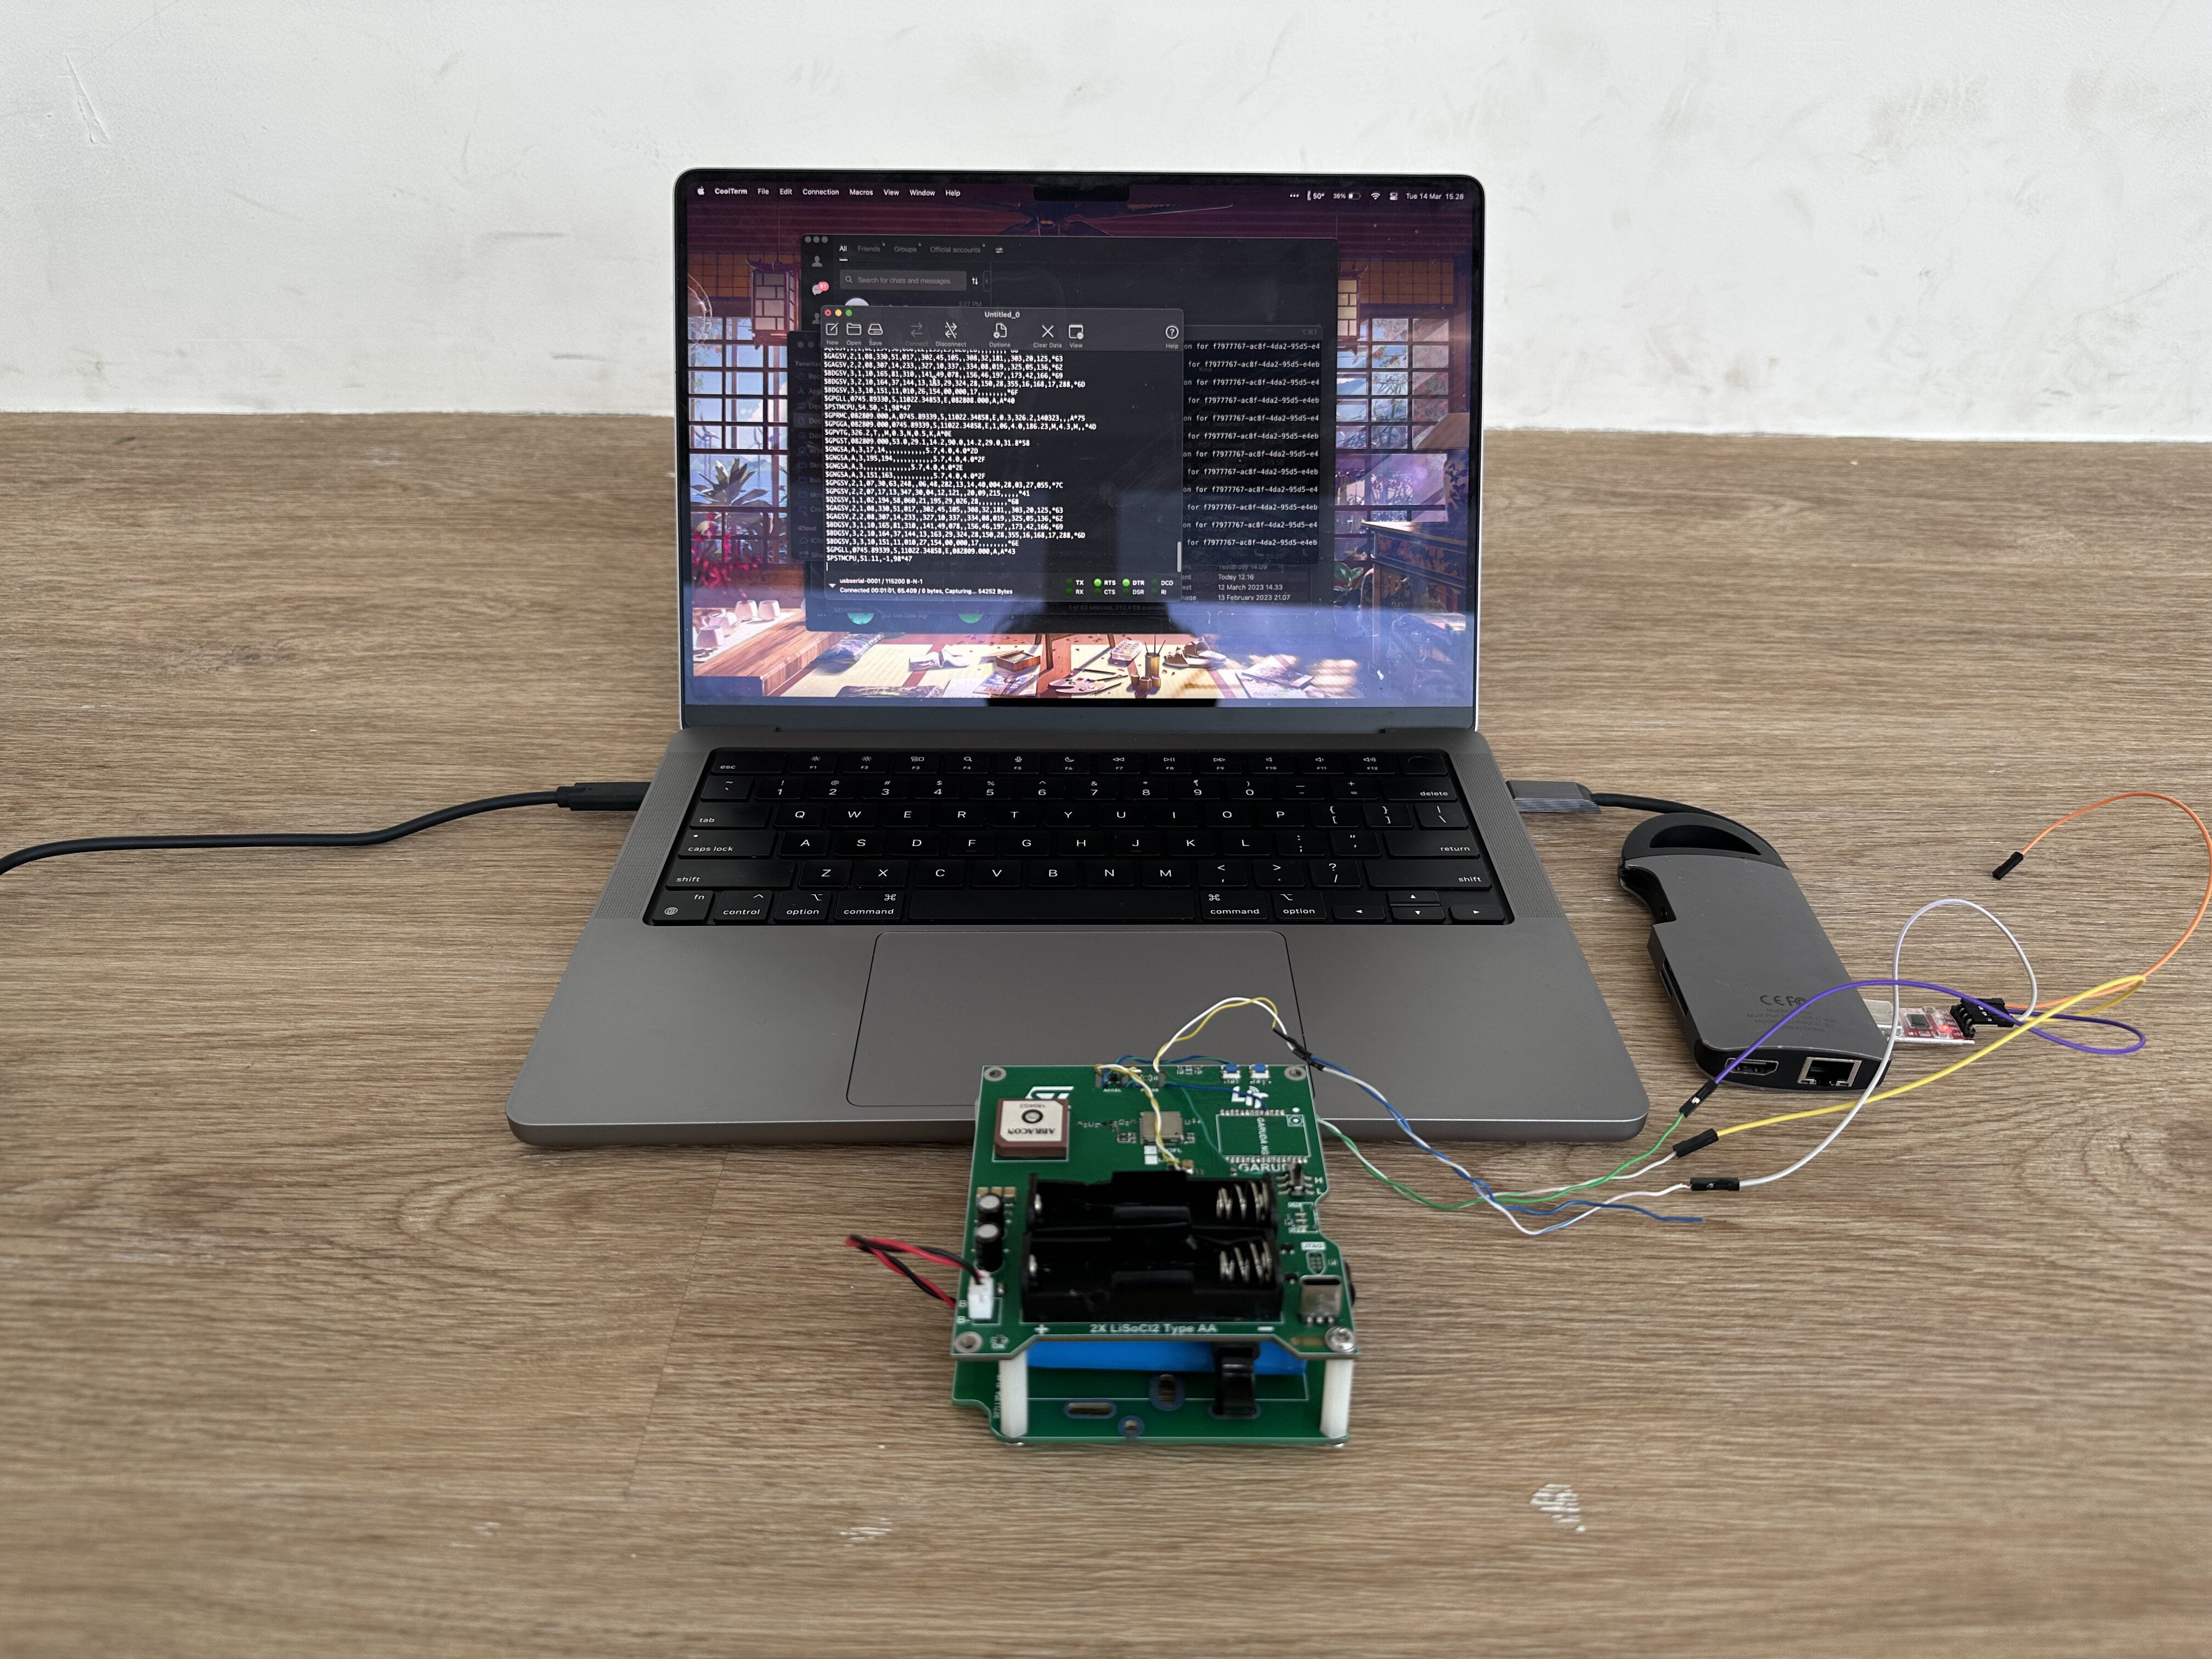
\includegraphics[width=10cm]{contents/chapter-4/2-skenario-indoor/keadaan.jpg}
	\caption{Keadaan sekitar pengujian skenario dalam ruangan}
	\label{Fig: indoor-keadaan}
\end{figure}

\subsection{Skenario Dalam Ruangan}
Pengujian skenario dilakukan di dalam ruangan tertutup pada lantai 5 Gedung SGLC Fakultas Teknik. Ruangan pengujian dilengkapi dengan jendela besar yang memungkinkan lebih banyak sinar matahari untuk masuk ke dalam ruangansehingga menghasilkan kondisi lingkungan yang cukup berbeda dengan pengujian skenario di \textit{basement}. Gambar \ref{Fig: indoor-keadaan} menunjukkan pengujian skenario dalam ruangan yang dilakukan pada penelitian ini.

\begin{figure}[H]
	\centering
	\begin{adjustbox}{width=\textwidth}
		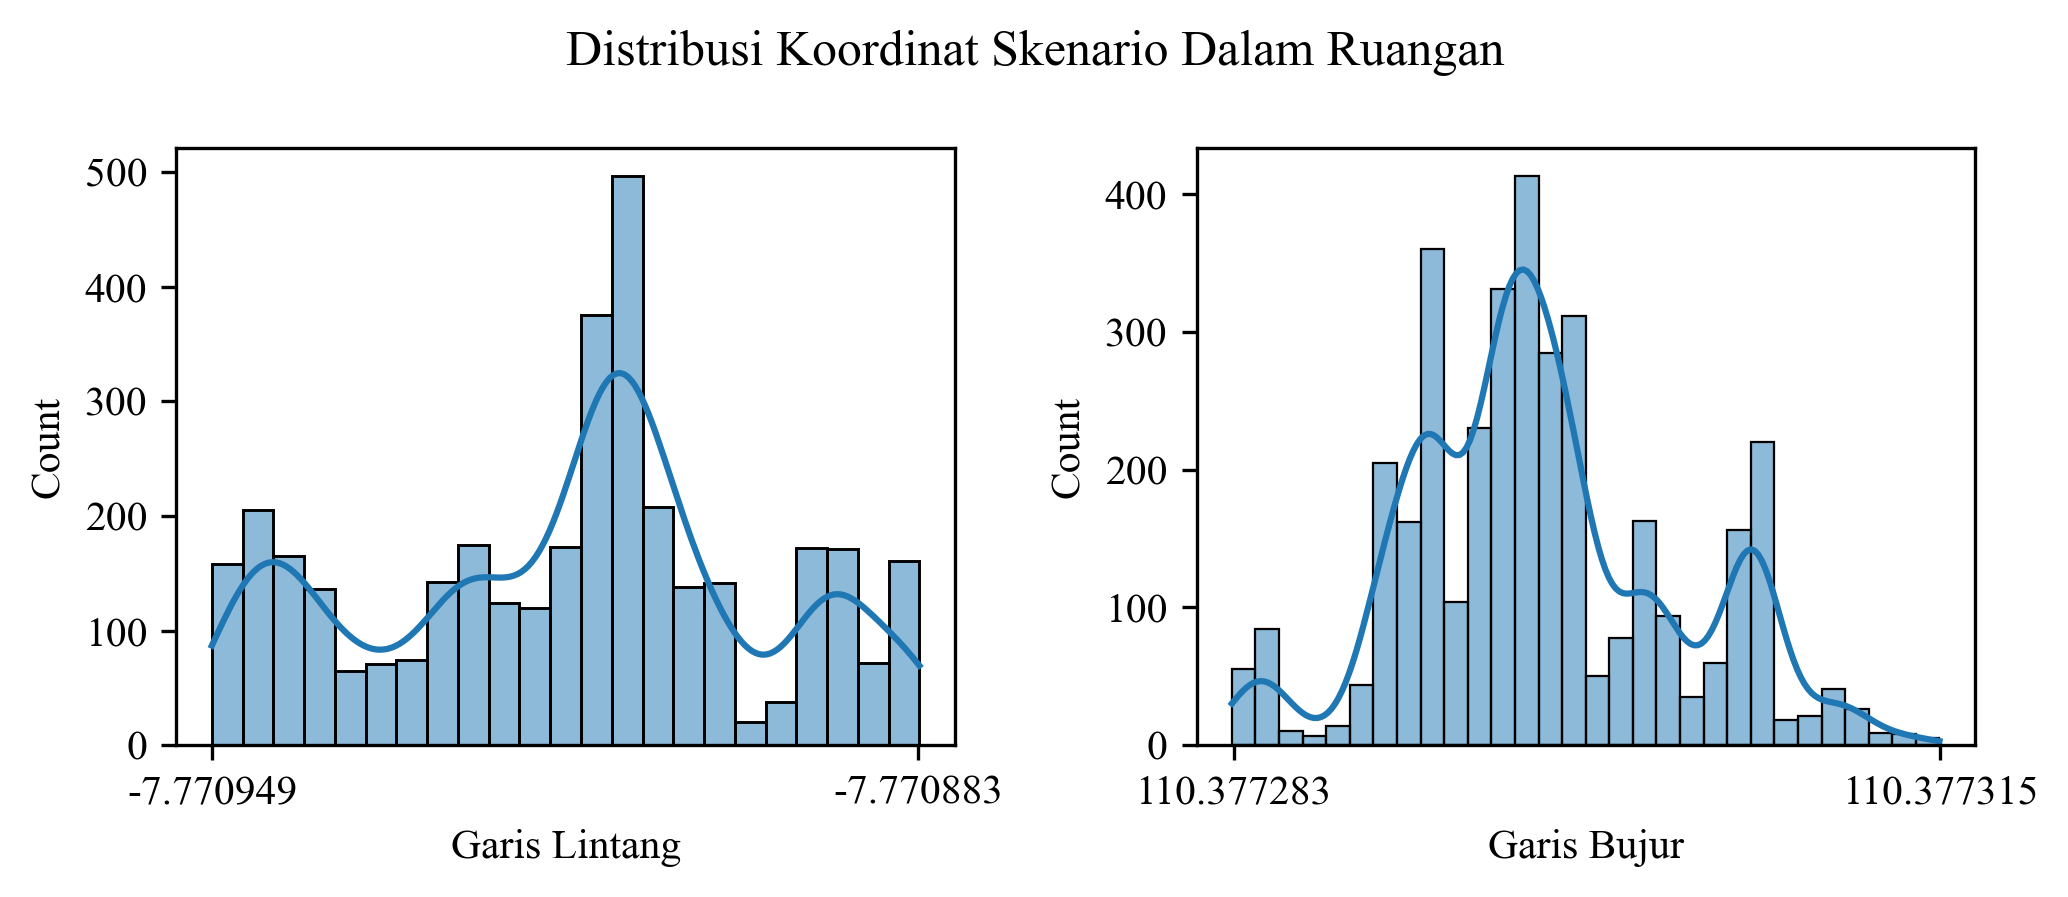
\includegraphics{contents/chapter-4/2-skenario-indoor/distribution.png}
	\end{adjustbox}
	\caption{Distribusi data koordinat skenario dalam ruangan}
	\label{Fig:indoor-distribution}
\end{figure}

Persebaran koordinat garis lintang dan garis bujur pada skenario dalam ruangan berada pada rentang -7,770949 hingga -7,770883 dan 110,377283 hingga 110,377315 seperti ditunjukan oleh Gambar \ref{Fig:indoor-distribution}. Namun, seperti halnya dengan skenario sebelumnya, distribusi koordinat pada pengujian ini tidak terdistribusi secara normalsehingga perlu dilakukan analisis pada nilai MAD-nya untuk mendapatkan pemahaman yang lebih baik mengenai data hasil pengujian.

\begin{table}[H]
	\caption{Hasil Pengujian Dalam Ruangan}
	\vspace{0.5em}
	\centering
	\begin{tabular}{ccccc}
		\hline
		& \textbf{Minima} & \textbf{Maxima} & \textbf{Rata-rata} & \textbf{Standar Deviasi}\\
		\hline 
		HDOP & 1,30 & 6,80 & 2,79 & 0,68\\
		VDOP & 1,40 & 5,50 & 2,48 & 0,94\\
		PDOP & 2,00 & 8,40 & 3,73 & 0,74\\
		CEP (m) & 9,51	& 33,27 & 12,14 & 4,02\\
		Jumlah Satelit & 8 & 15 & 10,93 & 1,14\\
		\hline
		\textbf{MAD-x (m)} & & \multicolumn{2}{c}{\centering 7,39} & \\
		\hline
		\textbf{MAD-y (m)} & & \multicolumn{2}{c}{\centering 4,11} & \\
		\hline
		\textbf{MAD (m)} & & \multicolumn{2}{c}{\centering 8,46} & \\
		\hline
	\end{tabular}
	\label{Tab: indoor-table}
\end{table}

Tabel \ref{Tab: indoor-table} menunjukan hasil pengujian pada skenario dalam ruangan. Penurunan nilai DOP menunjukan bahwa hasil pengukuran modul Teseo\hyp{}LIV3FL lebih akurat jika dibandingkan dengan skenario \textit{basement}. Selain itu, nilai MAD pada skenario ini juga menjadi lebih baik, yaitu 7,39 meter pada koordinat garis lintangnya, 4,11 meter pada garis bujurnya, dan 8,46 meter secara keseluruhan.

\begin{figure}[H]
	\centering
	\includegraphics[width=13cm]{contents/chapter-4/2-skenario-indoor/cep.png}
	\caption{CEP pengujian skenario dalam ruangan}
	\label{Fig: indoor-cep}
\end{figure}

Selain nilai MAD, grafik nilai CEP yang ditunjukan oleh Gambar \ref{Fig: indoor-cep} juga menunjukan bahwa tingkat presisi modul Teseo\hyp{}LIV3FL pada skenario ini lebih baik jika dibandingkan dengan percobaan sebelumnya. Nilai CEP terendah dapat mencapai 9,51 meter dan paling tinggi adalah sebesar 33,27 meter. Grafik nilai CEP pada skenario ini juga cenderung lebih stabil yang menyebabkan standar deviasi dari nilai CEP-nya menurun. 

\begin{figure}[H]
	\centering
	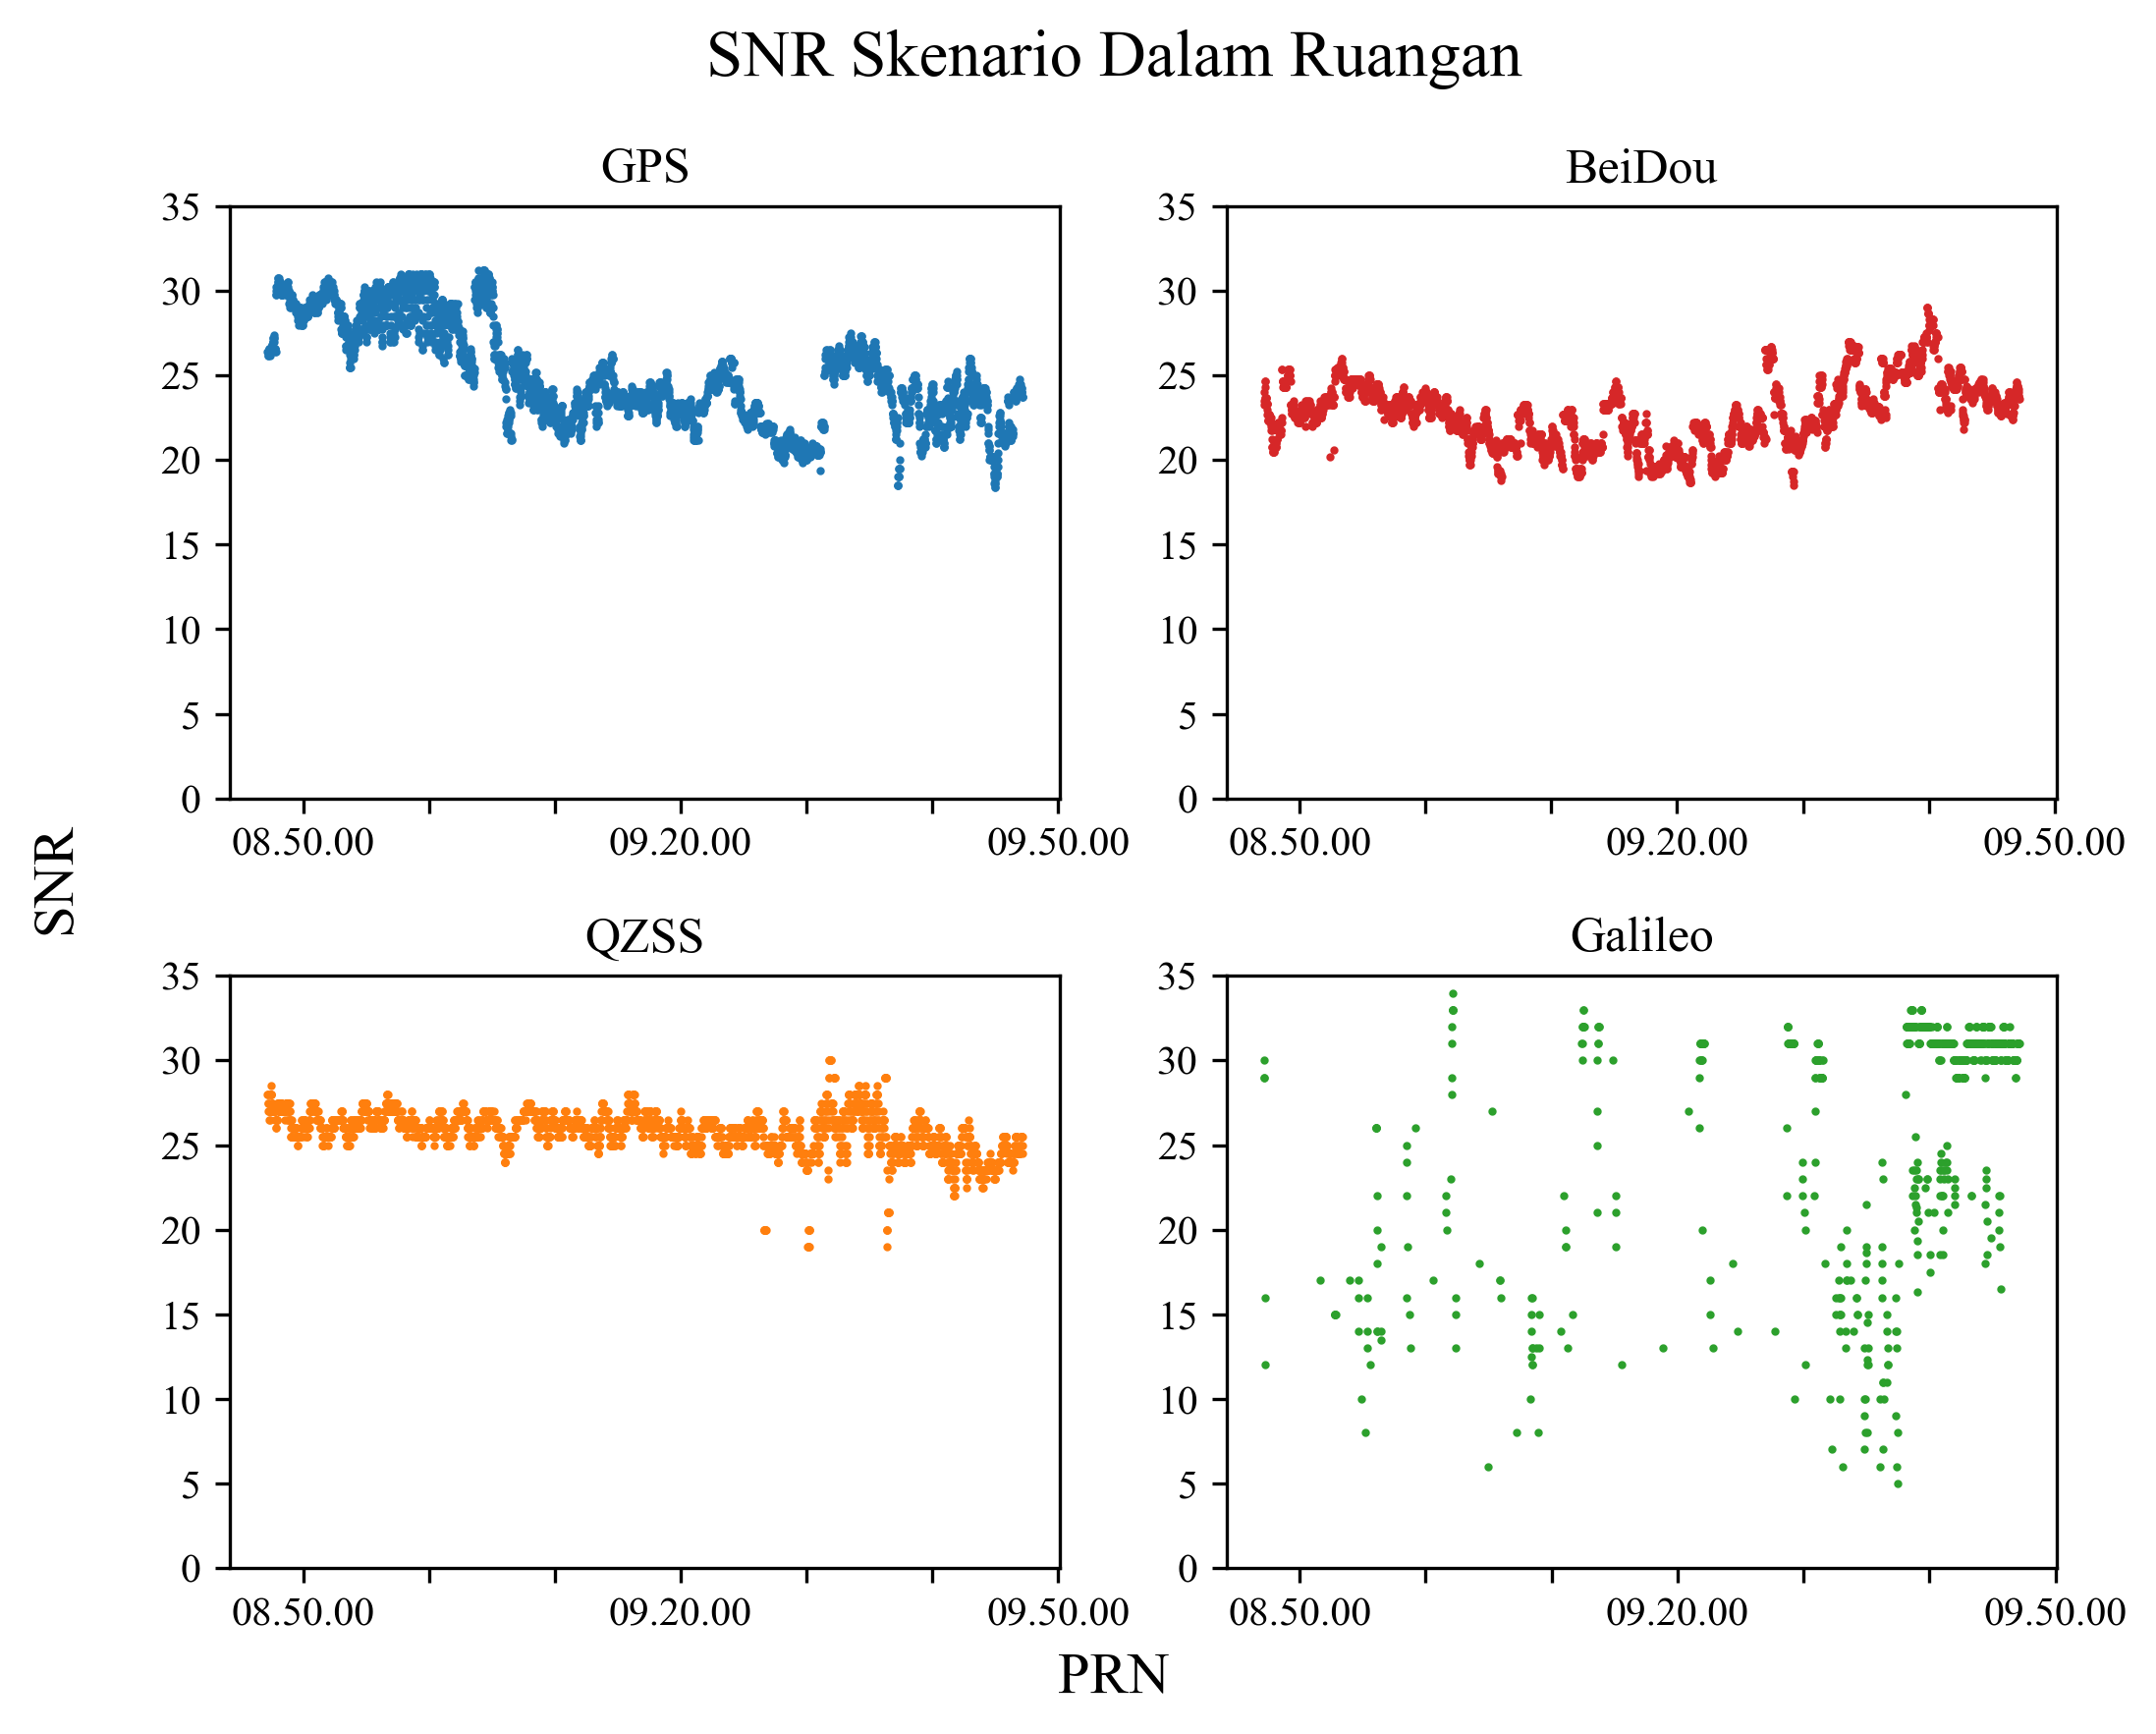
\includegraphics[width=13cm]{contents/chapter-4/2-skenario-indoor/snr.png}
	\caption{SNR setiap konstelasi pada pengujian skenario dalam ruangan}
	\label{Fig: indoor-snr}
\end{figure}

Pada akhir percobaan dapat dilihat bahwa terjadi lojakan nilai CEP meskipun jumlah visibilitas satelit pada periode waktu tersebut cenderung baik. Hal tersebut diakibatkan oleh penurunan nilai SNR yang cukup signifikan terjadi pada periode waktu tersebut. Grafik nilai SNR pada skenario ini ditunjukan oleh Gambar \ref{Fig: indoor-snr}. Konstelasi GPS cenderung mengalami penurunan seiring berjalannya waktu. Di sisi lain, konstelasi Galileo mengalami penurunan yang sangat signifikan hingga 5 dB. Selain itu, isyarat dari satelit konstelasi Galileo terkadang tidak dapat diterima oleh modul GNSS ditunjukan dengan beberapa titik yang kosong.

\begin{figure}[H]
	\centering
	\captionsetup{justification=centering}
	\begin{adjustbox}{width=\textwidth}
		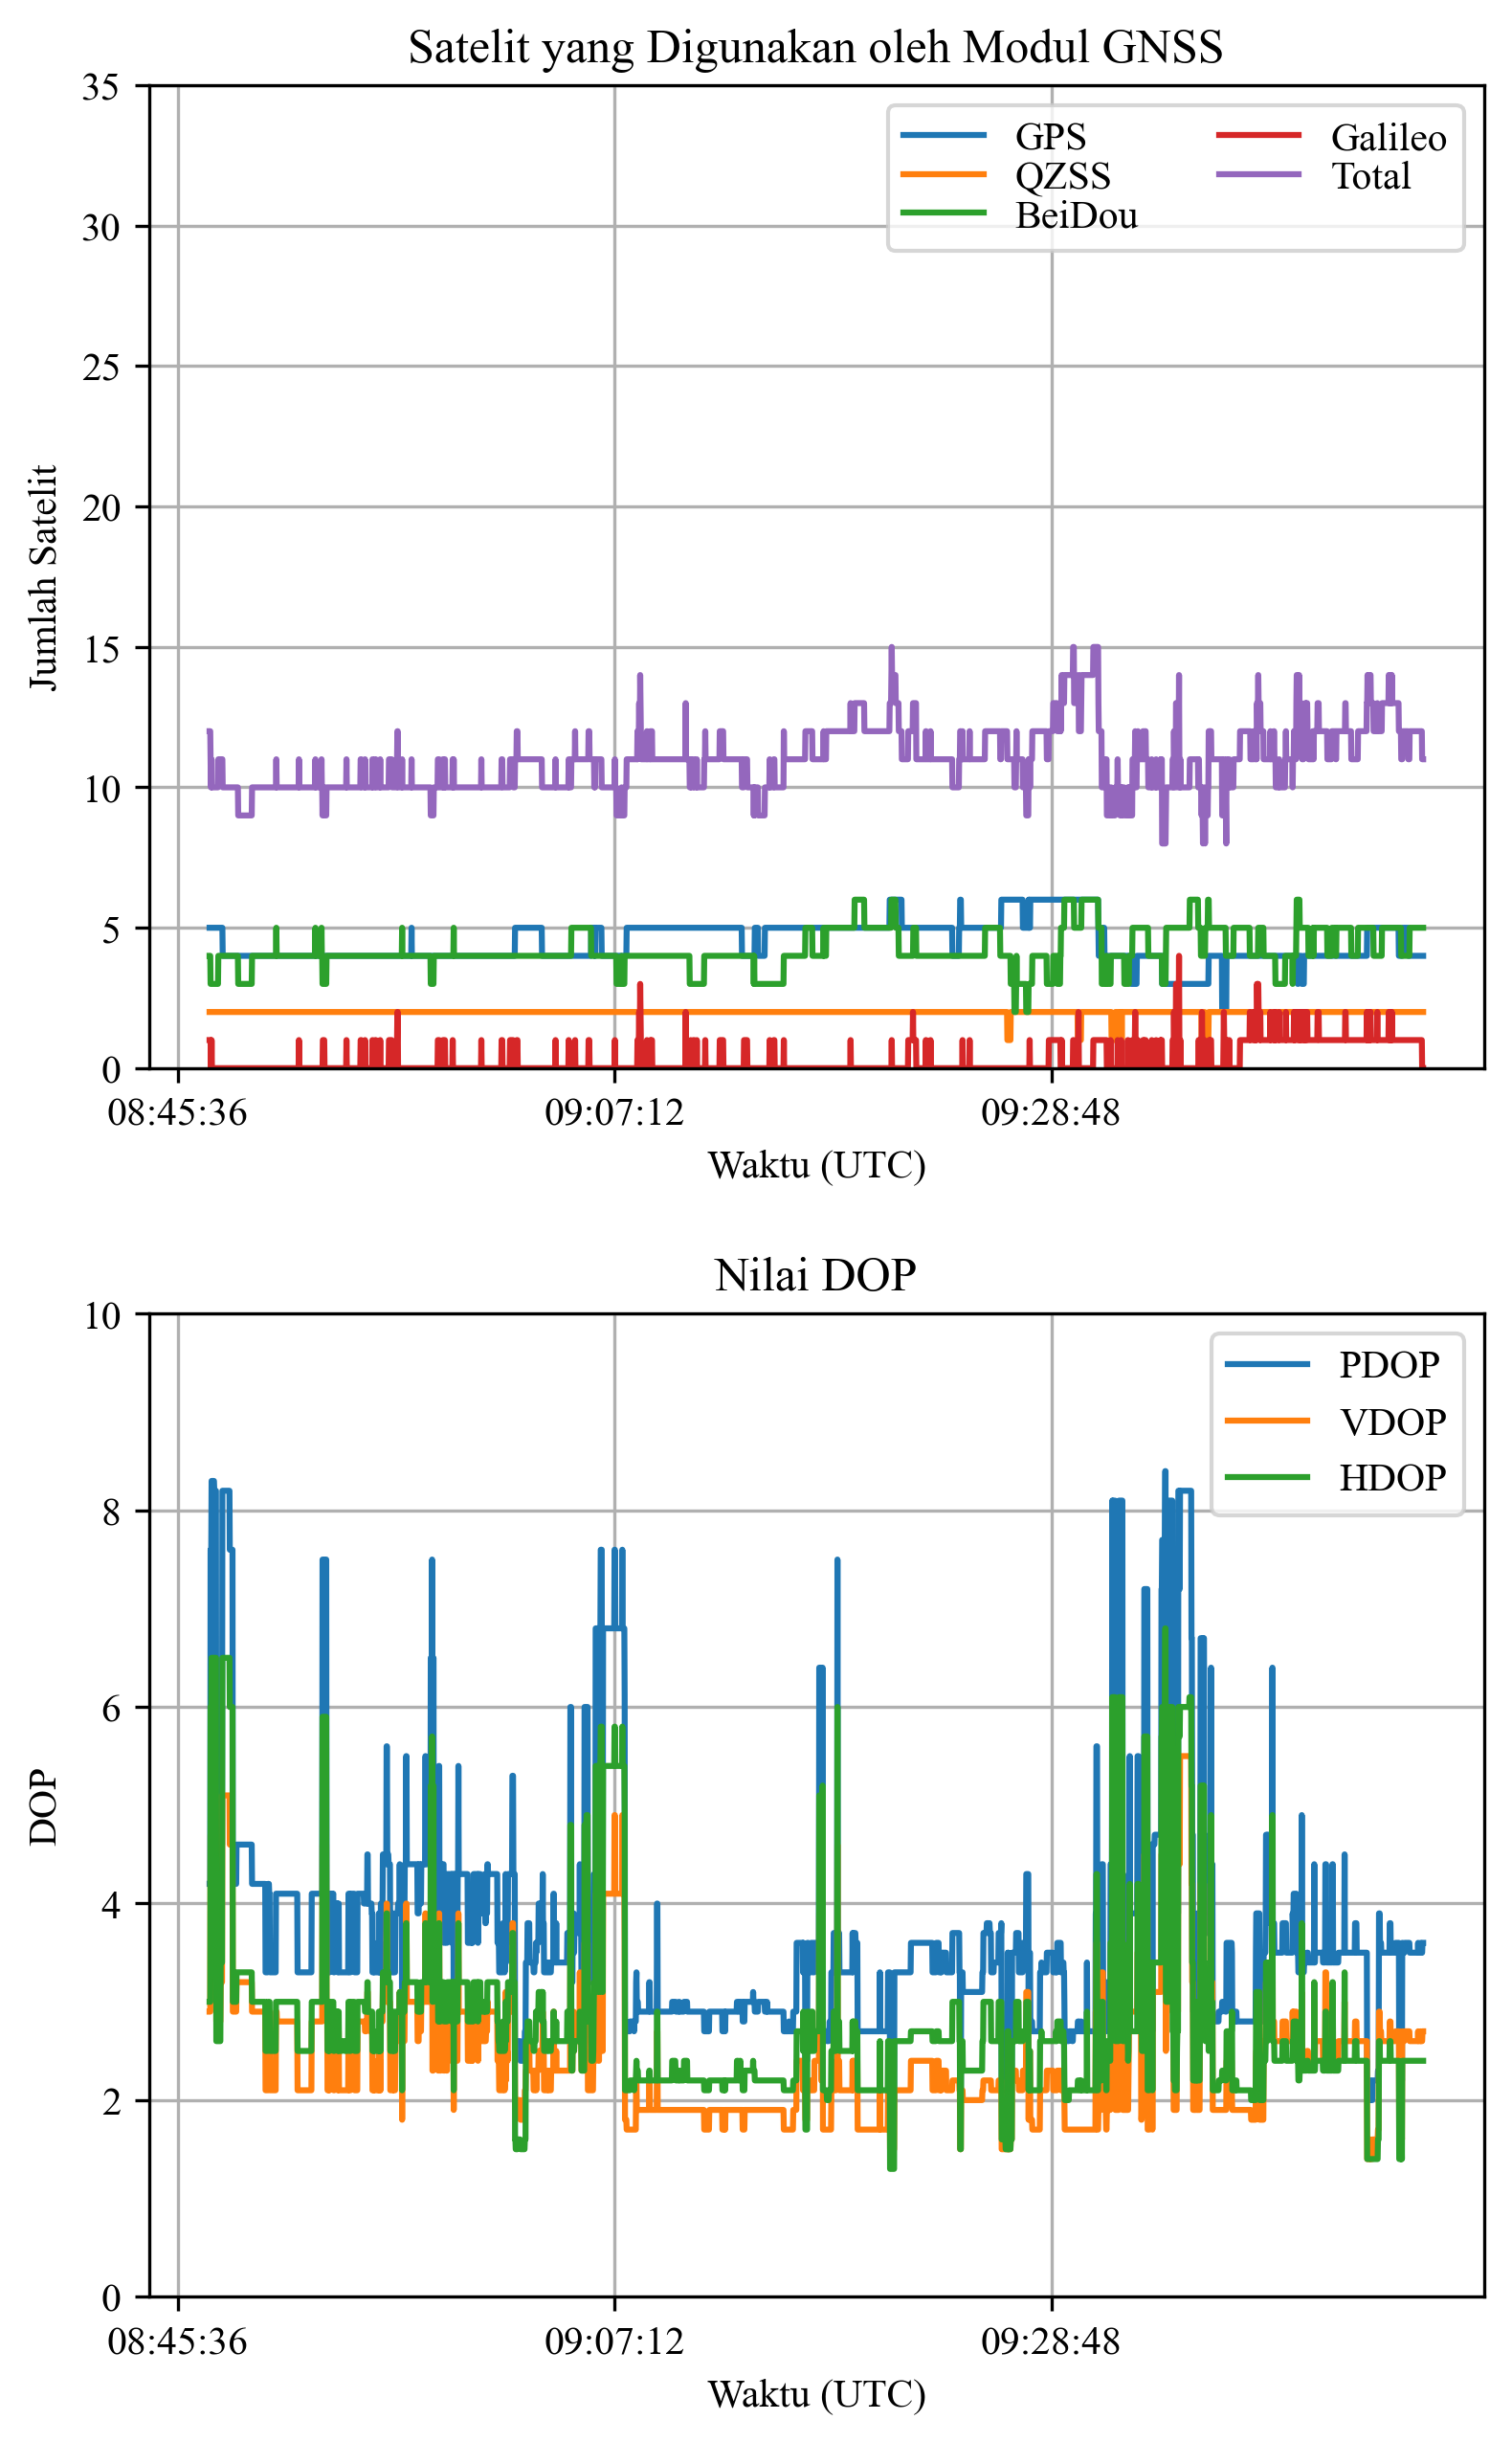
\includegraphics{contents/chapter-4/2-skenario-indoor/sats_dop.png}
	\end{adjustbox}
	\caption{DOP dan visibilitas satelit pengujian skenario dalam ruangan tertutup}
	\label{Fig: indoor-sats_dop}
\end{figure}

Sama seperti pada pengujian skenario \textit{basement}, modul Teseo\hyp{}LIV3FL juga dapat menerima isyarat dari keempat konstelasi yang telah diatur sebelumnya seperti ditunjukan pada Gambar \ref{Fig: indoor-sats_dop}. Dari hasil pengujian ini, terlihat bahwa konstelasi dengan jumlah satelit terbanyak adalah BeiDou dan GPS, yang dapat memberikan sinyal yang lebih kuat dan lebih akurat dalam mendukung navigasi satelit. Sementara itu, jumlah satelit pada konstelasi QZSS hampir selalu konstan pada dua buah satelit, sedangkan konstelasi Galileo dapat bervariasi antara nol hingga empat buah satelit tergantung pada kondisi lingkungan di sekitar pengujian. 

\begin{figure}[H]
	\centering
	\captionsetup{justification=centering}
	\includegraphics[width=12cm]{contents/chapter-4/2-skenario-indoor/sky_plot.png}
	\caption{\textit{Sky plot} skenario dalam ruangan}
	\label{Fig: indoor-sky_plot}
\end{figure}

\textit{Sky plot} pada Gambar \ref{Fig: indoor-sky_plot} menunjukan bahwa persebaran satelit pada skenario ini lebih tersebar merata jika dibandingkan dengan skenario sebelumnya. Persebaran satelit yang lebih baik tentunya berpengaruh terhadap tingkat akurasi dari modul Teseo\hyp{}LIV3FL. Tingkat persebaran satelit yang lebih tersebar juga sejalan dengan nilai PDOP pada Tabel \ref{Tab: indoor-table}. Hal tersebut dikarenakan nilai dari PDOP juga dipengaruhi oleh geometri dari satelit.

Tingkat kepresisian modul Teseo\hyp{}LIV3FL adalah sebesar 8,46 meter (MAD) dan 12,14 meter (CEP). Penurunan nilai CEP dan MAD pada skenario dalam ruangan jika dibandingkan pada skenario \textit{basement} menunjukan bahwa performa modul Teseo\hyp{}LIV3FL pada skenario ini lebih baik jika dibandingkan dengan skenario \textit{basement}. Rata-rata nilai HDOP pada pengujian ini adalah 2,79 yang menunjukan bahwa hasil pengukuran sudah baik dan tepat berada pada standar minimum pengukuran. Struktur beton yang lebih sedikit dapat membantu untuk meningkatkan performa GNSS terlihat pada semakin banyak satelit yang dapat digunakan dan penurunan pada nilai CEP dan ketiga nilai DOP.

\begin{figure}[H]
	\centering
	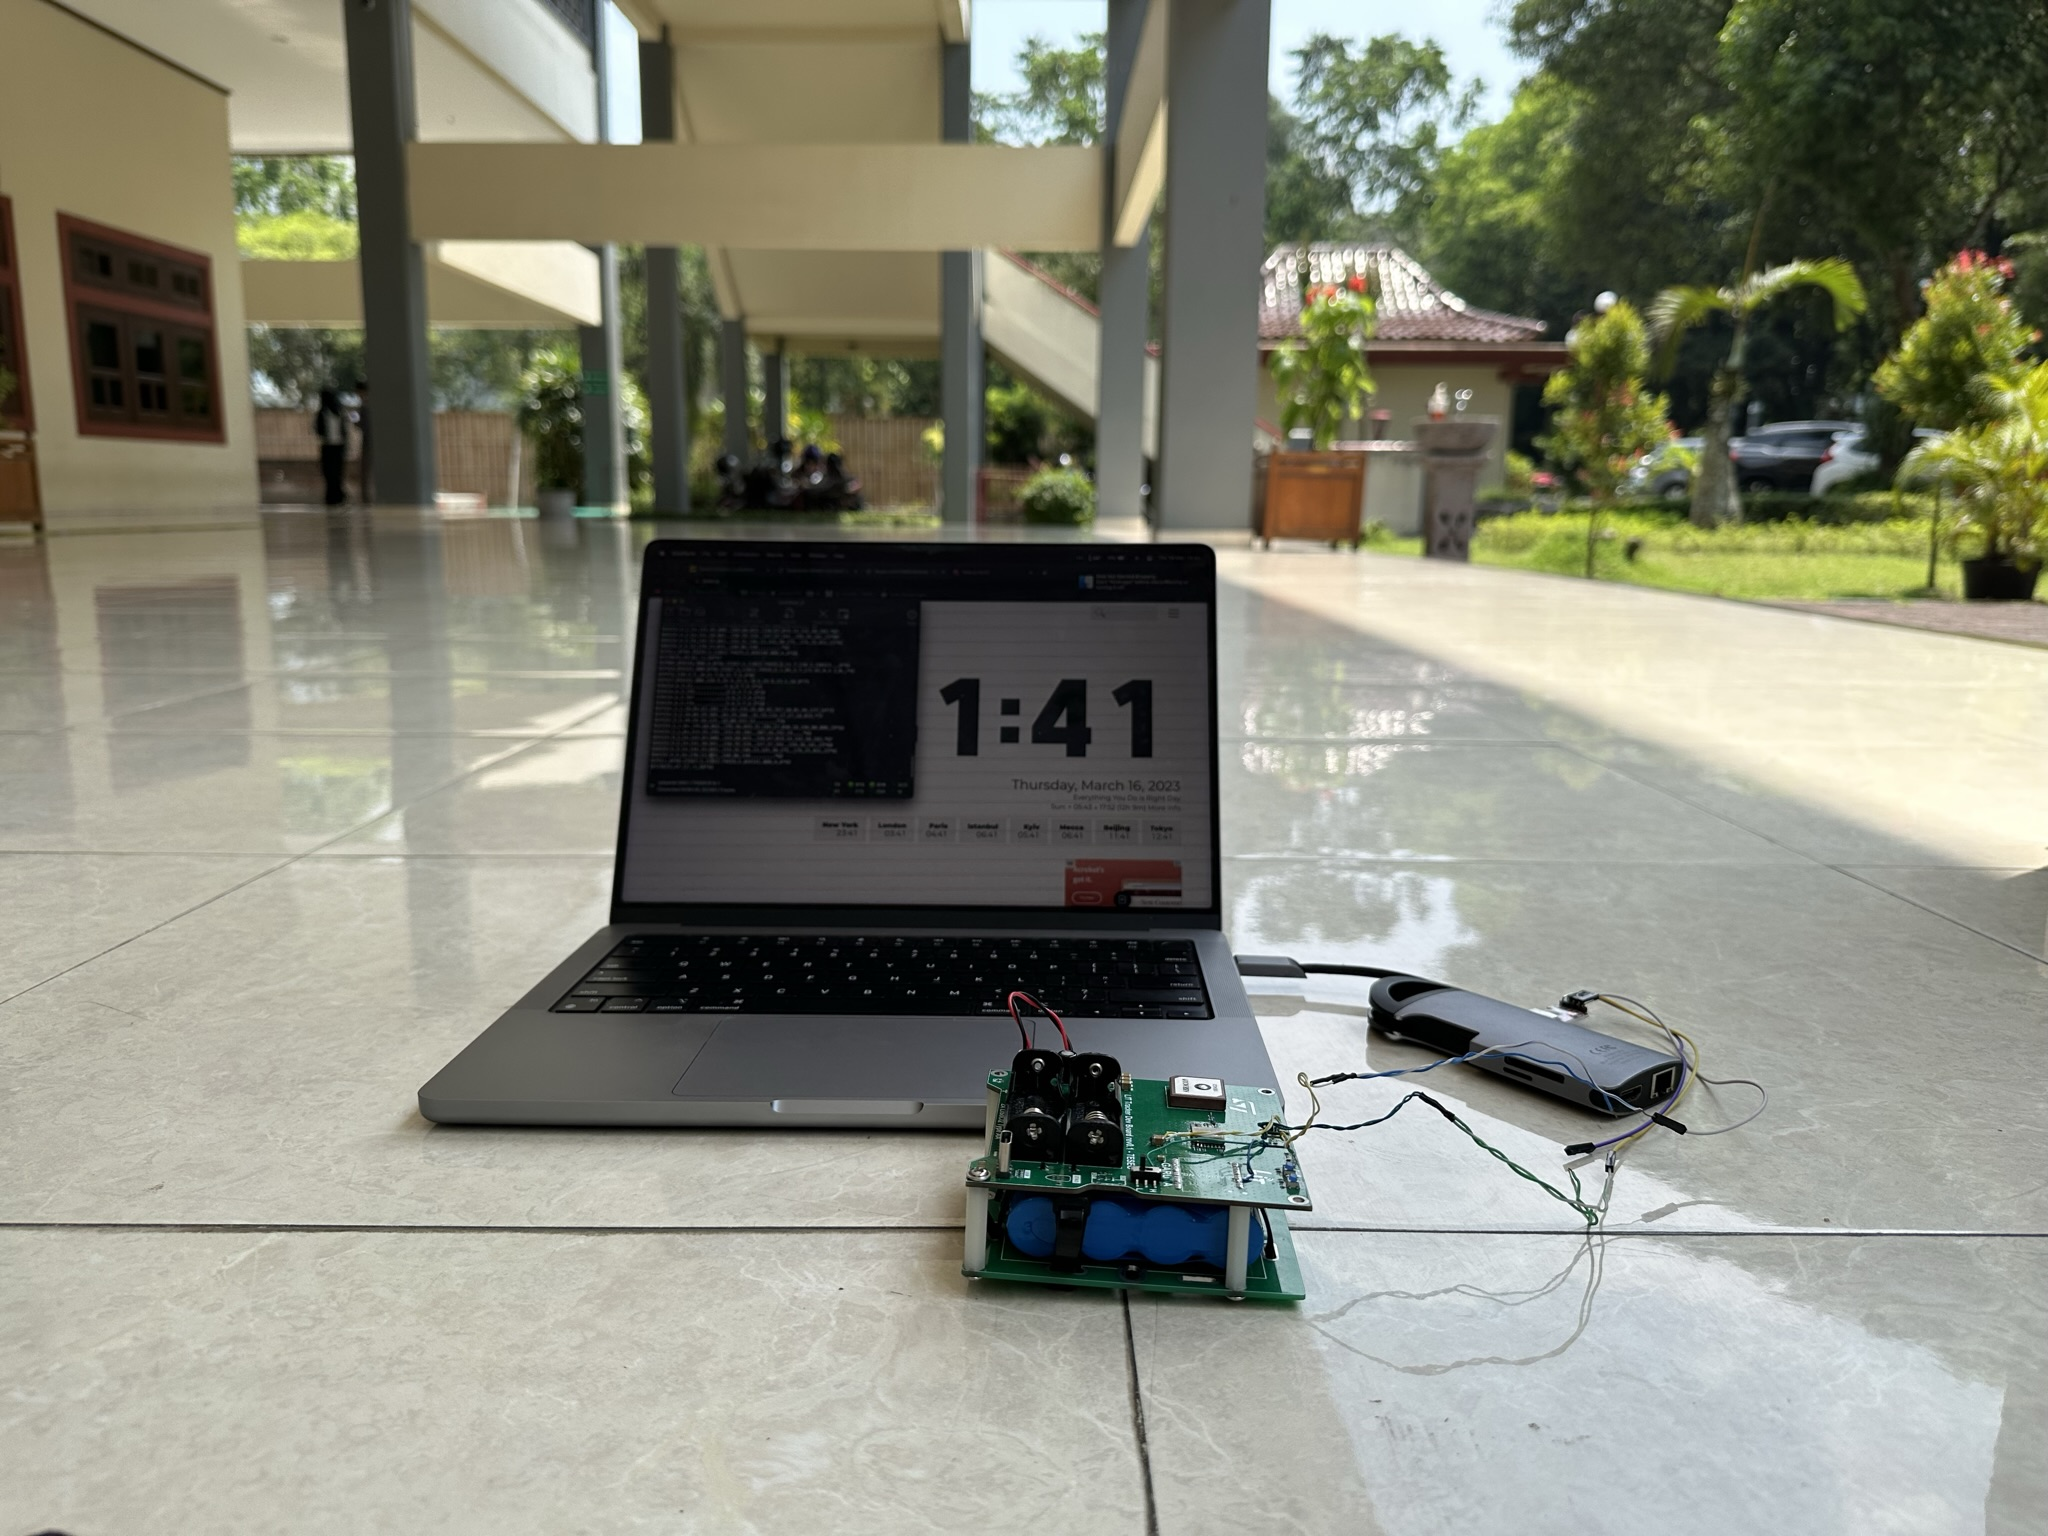
\includegraphics[width=10cm]{contents/chapter-4/3-skenario-semioutdoor/keadaan.jpeg}
	\caption{Keadaan sekitar pengujian skenario ruangan semi-terbuka}
	\label{Fig: semioutdoor-keadaan}
\end{figure}

\subsection{Skenario Ruangan Semi-Terbuka}
Pengujian skenario ruangan semi-terbuka dilakukan untuk mengevaluasi performa modul Teseo\hyp{}LIV3FL di luar ruangan dengan adanya penghalang seperti pohon, atap, dan lain sebagainya. Titik pengujian berada di Selasar Grha Sabha Pramana, sebuah ruangan semi-terbuka yang terdapat penghalang berupa tingkat dua Grha Sabha Pramana serta pepohonan yang berada di sekitar ruangan. Kondisi lingkungan yang ada pada pengujian ini jauh berbeda dengan pengujian dalam ruangan atau pengujian di \textit{basement}. Gambar \ref{Fig: semioutdoor-keadaan} menunjukan pengujian skenario ruangan semi terbuka.

\begin{figure}[H]
	\centering
	\begin{adjustbox}{width=\textwidth}
		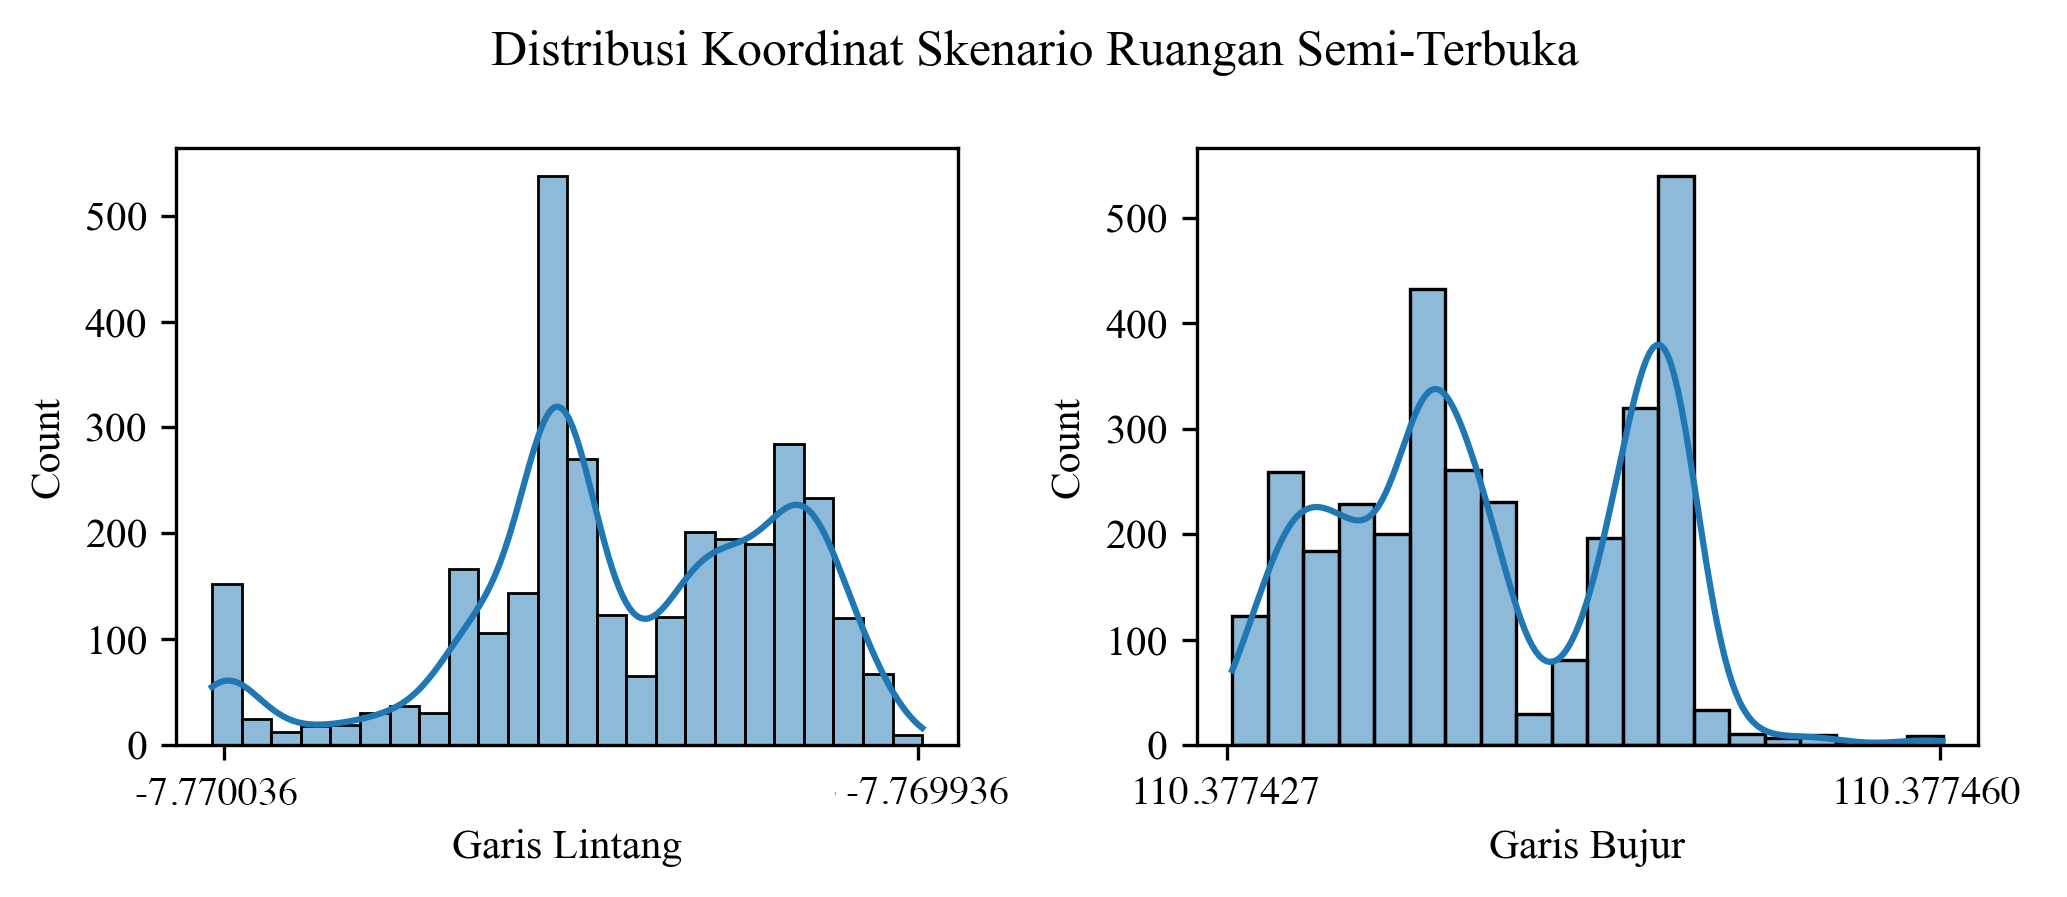
\includegraphics{contents/chapter-4/3-skenario-semioutdoor/distribution.png}
	\end{adjustbox}
	\caption{Distribusi data koordinat skenario ruangan semi-terbuka}
	\label{Fig:semioutdoor-distribution}
\end{figure}

Sama seperti hasil pengujian pada dua skenario sebelumnya, data koordinat garis lintang dan garis bujur pada pengujian skenario ruang semi terbuka tidak terdistribusi normal seperti ditunjukan oleh \textit{kernel density estimator} Gambar \ref{Fig:semioutdoor-distribution}. Oleh karena itu, pada pengujian ini juga akan dilakukan analisis statistik non-parametrik terhadap nilai MAD-nya. Nilai koordinat garis lintang pada pengujian ini berada pada rentang -7,770036 hingga -7,769936 dan 110,377427 hingga 110,377460 untuk koordinat garis bujurnya.

\begin{table}[H]
	\caption{Hasil Pengujian di Ruangan Semi Terbuka}
	\vspace{0.5em}
	\centering
	\begin{tabular}{ccccc}
		\hline
		& \textbf{Minima} & \textbf{Maxima} & \textbf{Rata-rata} & \textbf{Standar Deviasi}\\
		\hline 
		HDOP & 0,70 & 1,30 & 0,83 & 0,06\\
		VDOP & 1,10	& 2,10 & 1,35 & 0,13\\
		PDOP & 1,30	& 2,30 & 1,58 & 0,13\\
		CEP (m) & 7,09	& 19,09 & 7,60 & 0,96\\
		Jumlah Satelit & 14 & 19 & 16,68 & 0,92\\
		\hline
		\textbf{MAD-x (m)} & & \multicolumn{2}{c}{\centering 1,60} & \\
		\hline
		\textbf{MAD-y (m)} & & \multicolumn{2}{c}{\centering 0,96} & \\
		\hline
		\textbf{MAD (m)} & & \multicolumn{2}{c}{\centering 1,87} & \\
		\hline
	\end{tabular}
	\label{Tab: semioutdoor-table}
\end{table}

Pada hasil pengujian yang ditunjukan oleh Tabel \ref{Tab: outdoor-table}, ditemukan bahwa terjadi penurunan pada ketiga nilai DOP seiring dengan peningkatan jumlah satelit yang digunakan, yang menunjukkan bahwa akurasi dari modul Teseo\hyp{}LIV3FL semakin meningkat. Selain itu, nilai MAD dari modul ini juga mengalami penurunan yang signifikan, dengan nilai 1,60 meter pada koordinat garis lintang, 0,96 meter pada koordinat garis bujur, dan 1,87 meter untuk MAD secara keseluruhan.

\begin{figure}[H]
	\centering
	\includegraphics[width=13cm]{contents/chapter-4/3-skenario-semioutdoor/cep.png}
	\caption{CEP pengujian skenario ruang semi-terbuka}
	\label{Fig: semioutdoor-cep}
\end{figure}

Grafik nilai CEP yang ditunjukan oleh Gambar \ref{Fig: semioutdoor-cep} juga menunjukan bahwa terjadi peningkatan tingkat kepresisian jika dibandingkan dengan dua skenario sebelumnya. Pada skenario ini, nilai CEP paling rendah dapat menyentuh angka 7,09 meter. Secara visual, nilai CEP pada skenario ini sempat berada dalam titik tertingginya dan menurun hinggai mencapai \textit{steady state} pada pukul 02.55.00 UTC. Standar deviasi yang rendah menunjukan bahwa nilai CEP-nya sangat dekat dengan rata-ratanya.

\begin{figure}[H]
	\centering
	\captionsetup{justification=centering}
	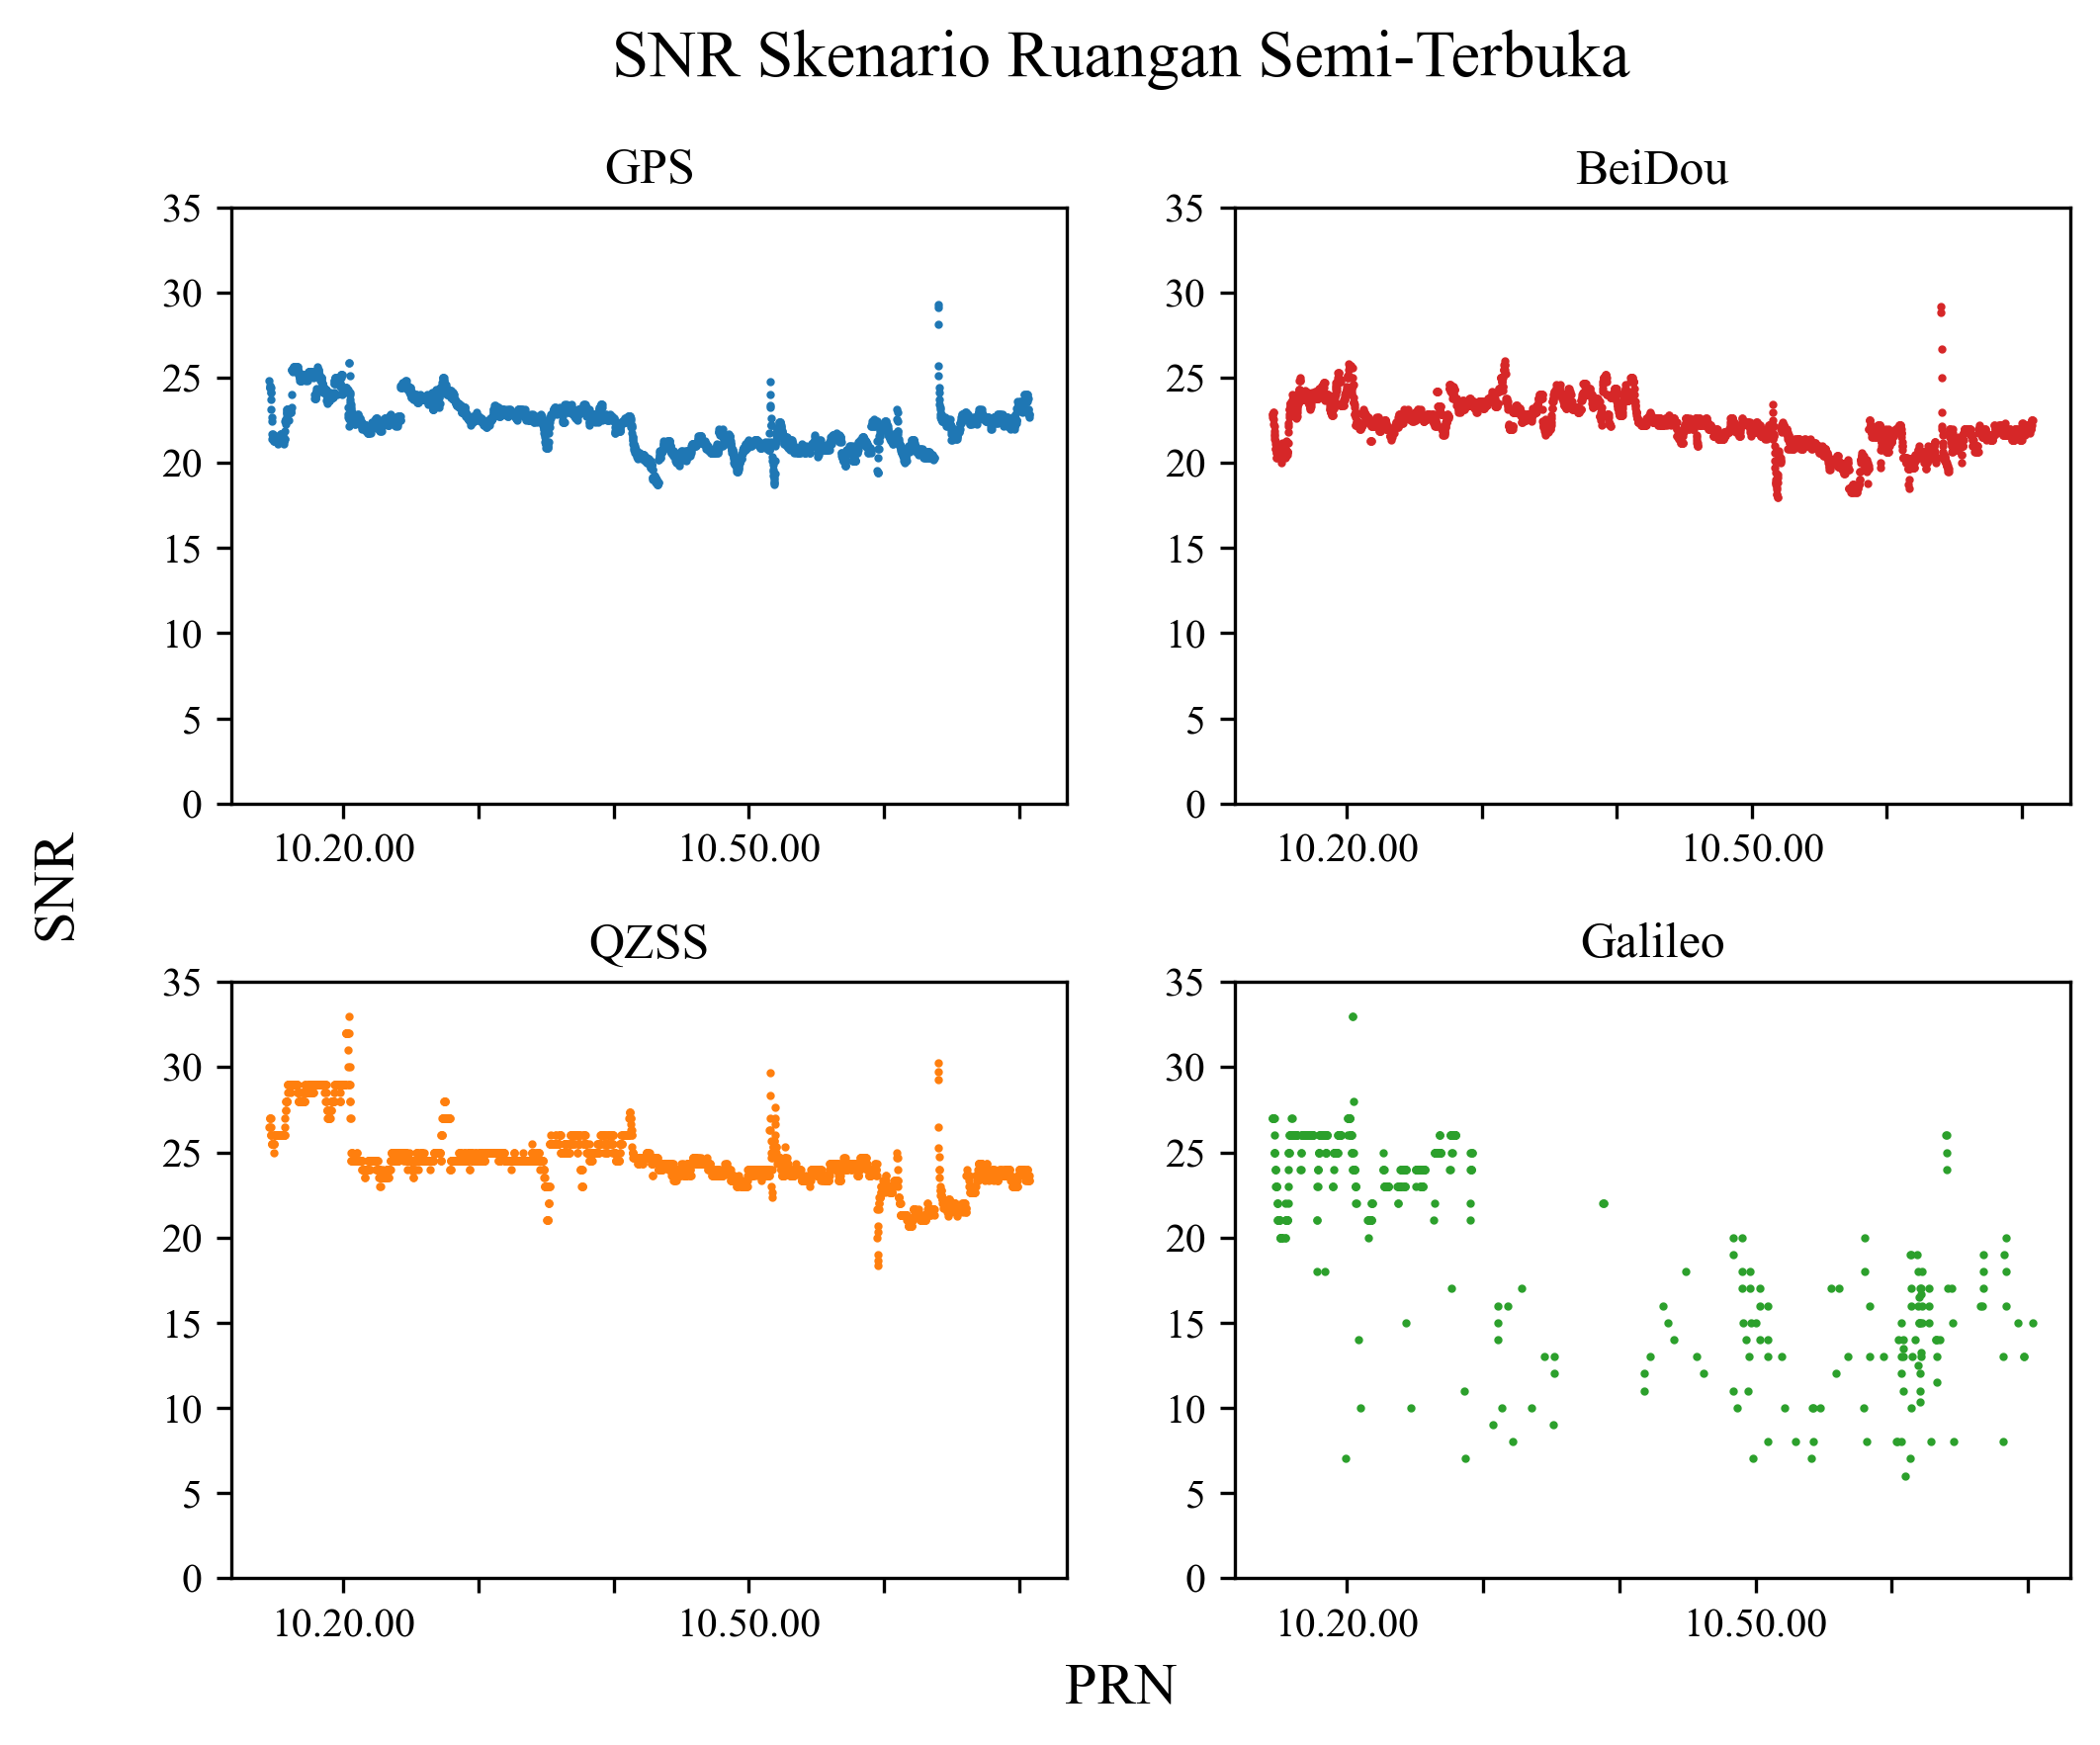
\includegraphics[width=13cm]{contents/chapter-4/3-skenario-semioutdoor/snr.png}
	\caption{SNR setiap konstelasi pada pengujian skenario ruang semi-terbuka}
	\label{Fig: semioutdoor-snr}
\end{figure}

Jika dilihat pada grafik SNR-nya, seluruh konstelasi GNSS selain Galileo memiliki nilai SNR yang relatif stabil seperti ditunjukan oleh Gambar \ref{Fig: semioutdoor-snr}. Dapat dilihat bahwa pada konstelasi QZSS menunjukan nilai SNR yang paling tinggi, tetapi karena visibilitas satelitnya tidak sebanyak GPS dan BeiDou maka tidak memberikan pengaruh yang cukup signifikan. Jika diperhatikan, SNR pada konstelasi Galileo sangatlah fluktuatif. Hal tersebut bersamaan dengan visibilitas satelitnya yang juga cenderung fluktuatif.

\begin{figure}[H]
	\centering
	\captionsetup{justification=centering}
	\begin{adjustbox}{width=\textwidth}
		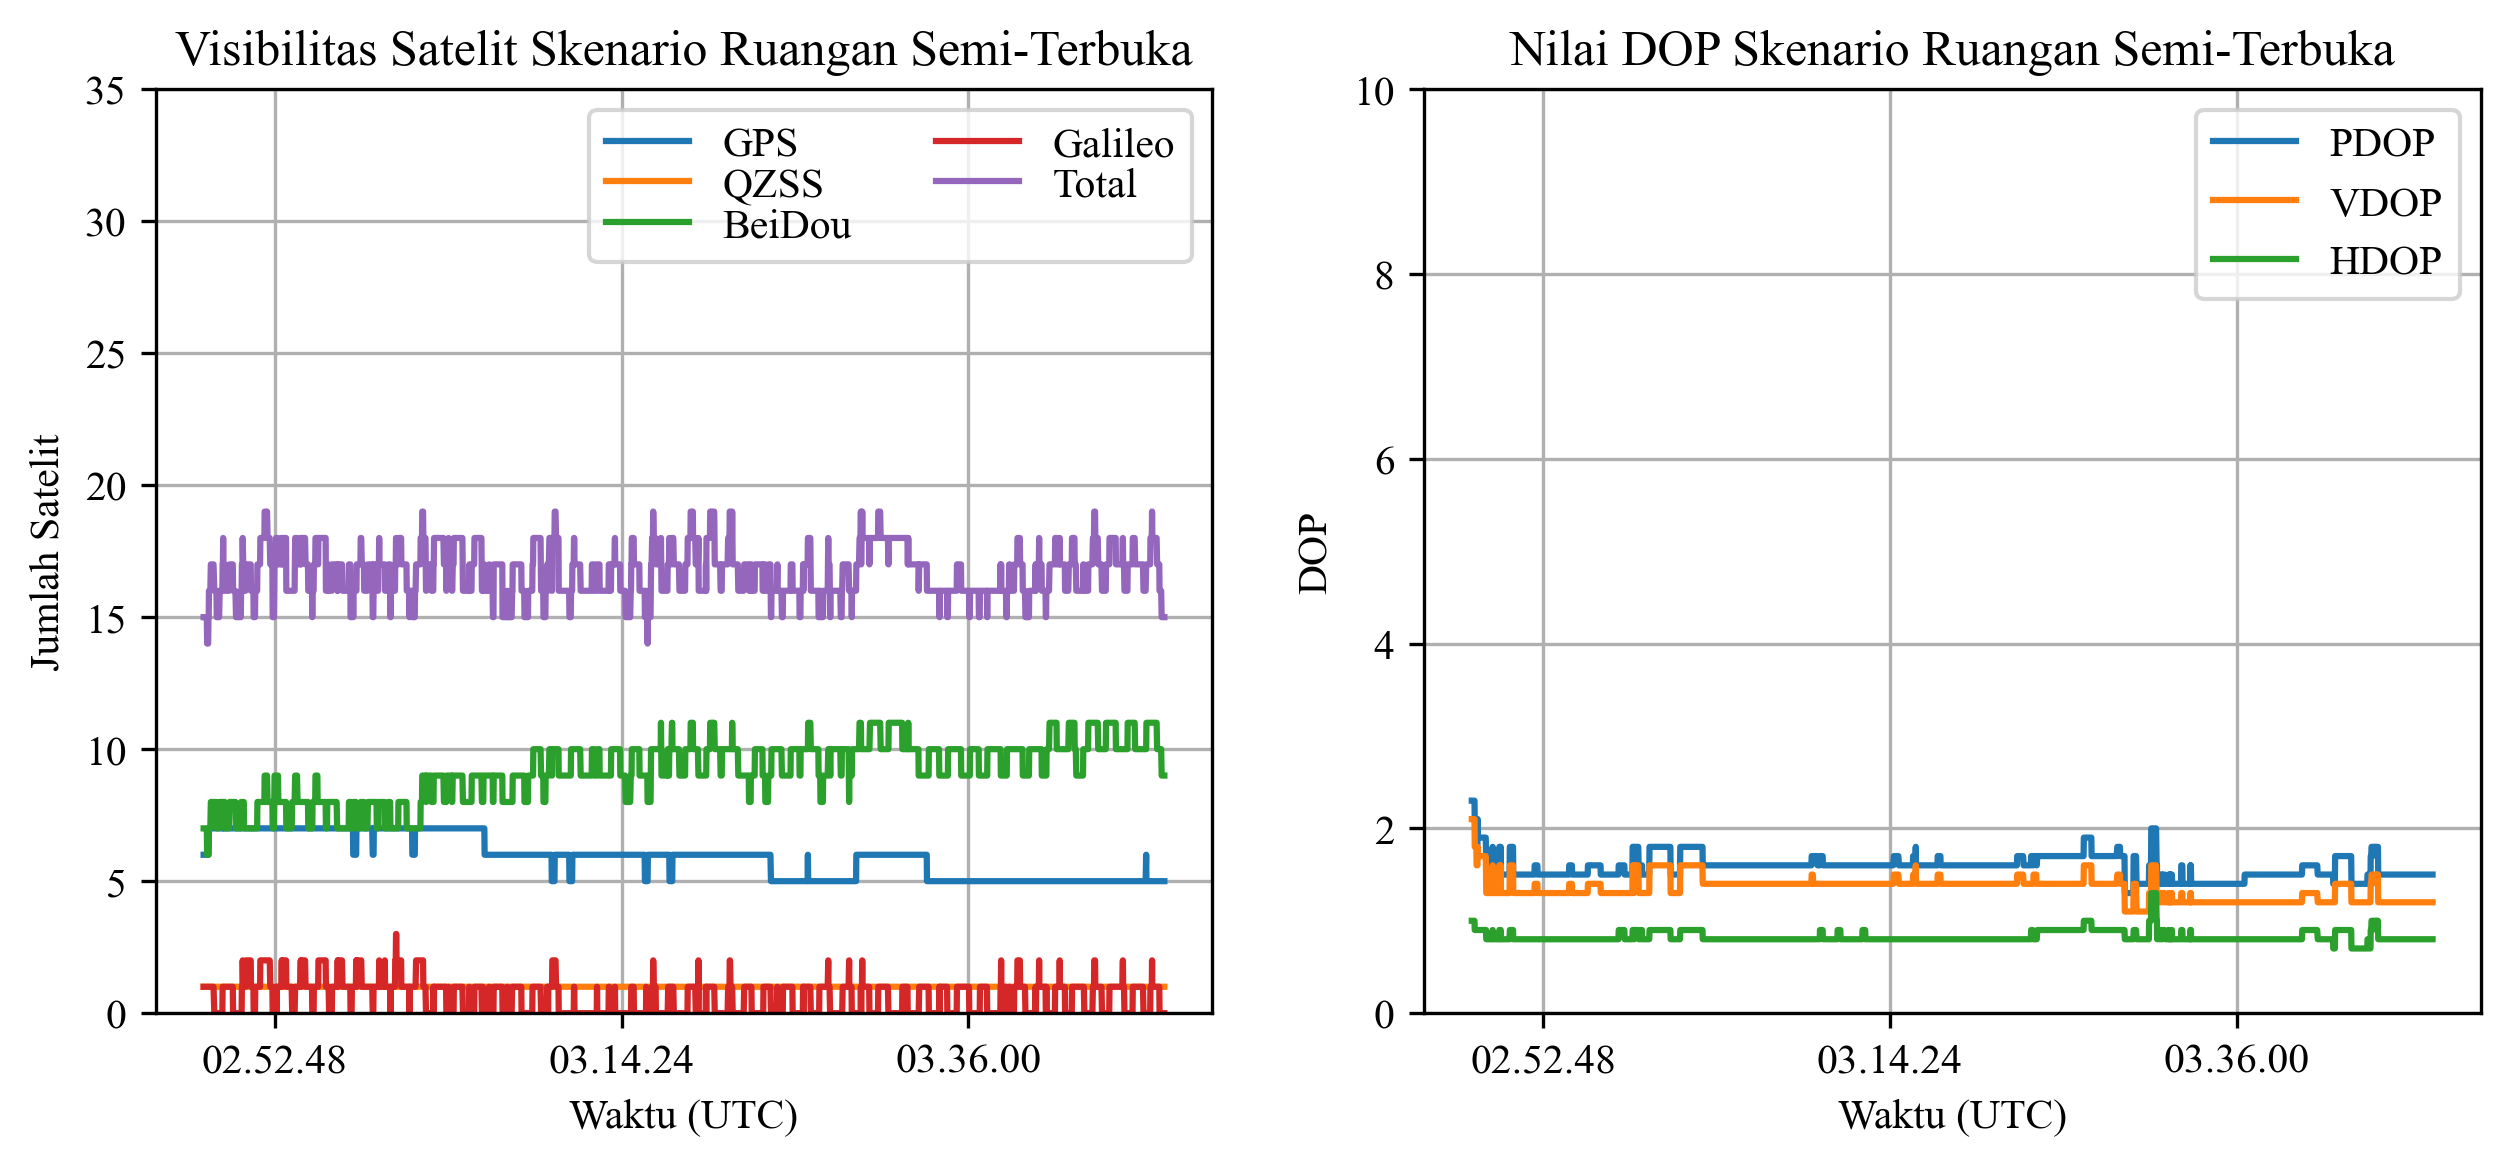
\includegraphics{contents/chapter-4/3-skenario-semioutdoor/sats_dop.png}
	\end{adjustbox}
	\caption{DOP dan visibilitas satelit pengujian skenario ruangan semi-terbuka}
	\label{Fig: semioutdoor-sats_dop}
\end{figure}

Pada pengujian ini, urutan konstelasi dengan jumlah satelit paling banyak hingga paling sedikit adalah GPS, BeiDou, QZSS, dan BeiDou. Rata-rata jumlah satelit yang digunakan adalah 16,68 dengan jumlah terbanyak 19 buah seperti ditunjukan pada Tabel \ref{Tab: semioutdoor-table}. Visibilitas satelit pada skenario ruangan semi terbuka lebih baik jika dibandingkan dengan dua skenario sebelumnya. Gambar \ref{Fig: semioutdoor-sats_dop} menunjukan bahwa konstelasi dengan visibilitas satelit paling banyak adalah konstelasi BeiDou dan GPS.

\begin{figure}[H]
	\centering
	\captionsetup{justification=centering}
	\includegraphics[width=12cm]{contents/chapter-4/3-skenario-semioutdoor/sky_plot.png}
	\caption{\textit{Sky plot} skenario ruangan semi-terbuka}
	\label{Fig: semioutdoor-sky_plot}
\end{figure}


Jika ditinjau dari nilai DOP, ketiga nilai DOP juga mengalami penurunan secara signifikan. Penurunan nilai HDOP menunjukan terdapat peningkatan akurasi pada hasil pembacaan di bidang horizontal, sedangkan penurunan nilai VDOP menunjukan peningkatan akurasi pada pembacaan ketinggian. Gambar \ref{Fig: semioutdoor-sky_plot} menunjukan persebaran satelit di langit sudah mencakup seluruh kuadran lingkaran. Hal tersebut juga didukung oleh nilai PDOP yang lebih rendah.

Berdasarkan hasil yang didapat, pada pengujian skenario ini dapat dilihat bahwa penempatan modul Teseo\hyp{}LIV3FL pada lingkungan dengan penghalang yang lebih sedikit dapat meningkatkan tingkat akurasinya. Rata-rata nilai PDOP dan VDOP sudah berada dalam rentang sangat baik dan HDOP berada dalam rentang ideal yang artinya sudah dapat digunakan dalam aplikasi yang sensitif terhadap ketelitian. Selain itu, nilai MAD pada skenario ini adalah 1,87 meter dan 7,60 meter untuk CEP. Penurunan nilai CEP dan MAD menunjukan bahwa terjadi peningkatan pada tingkat kepresisiannya.

\begin{figure}[H]
	\centering
	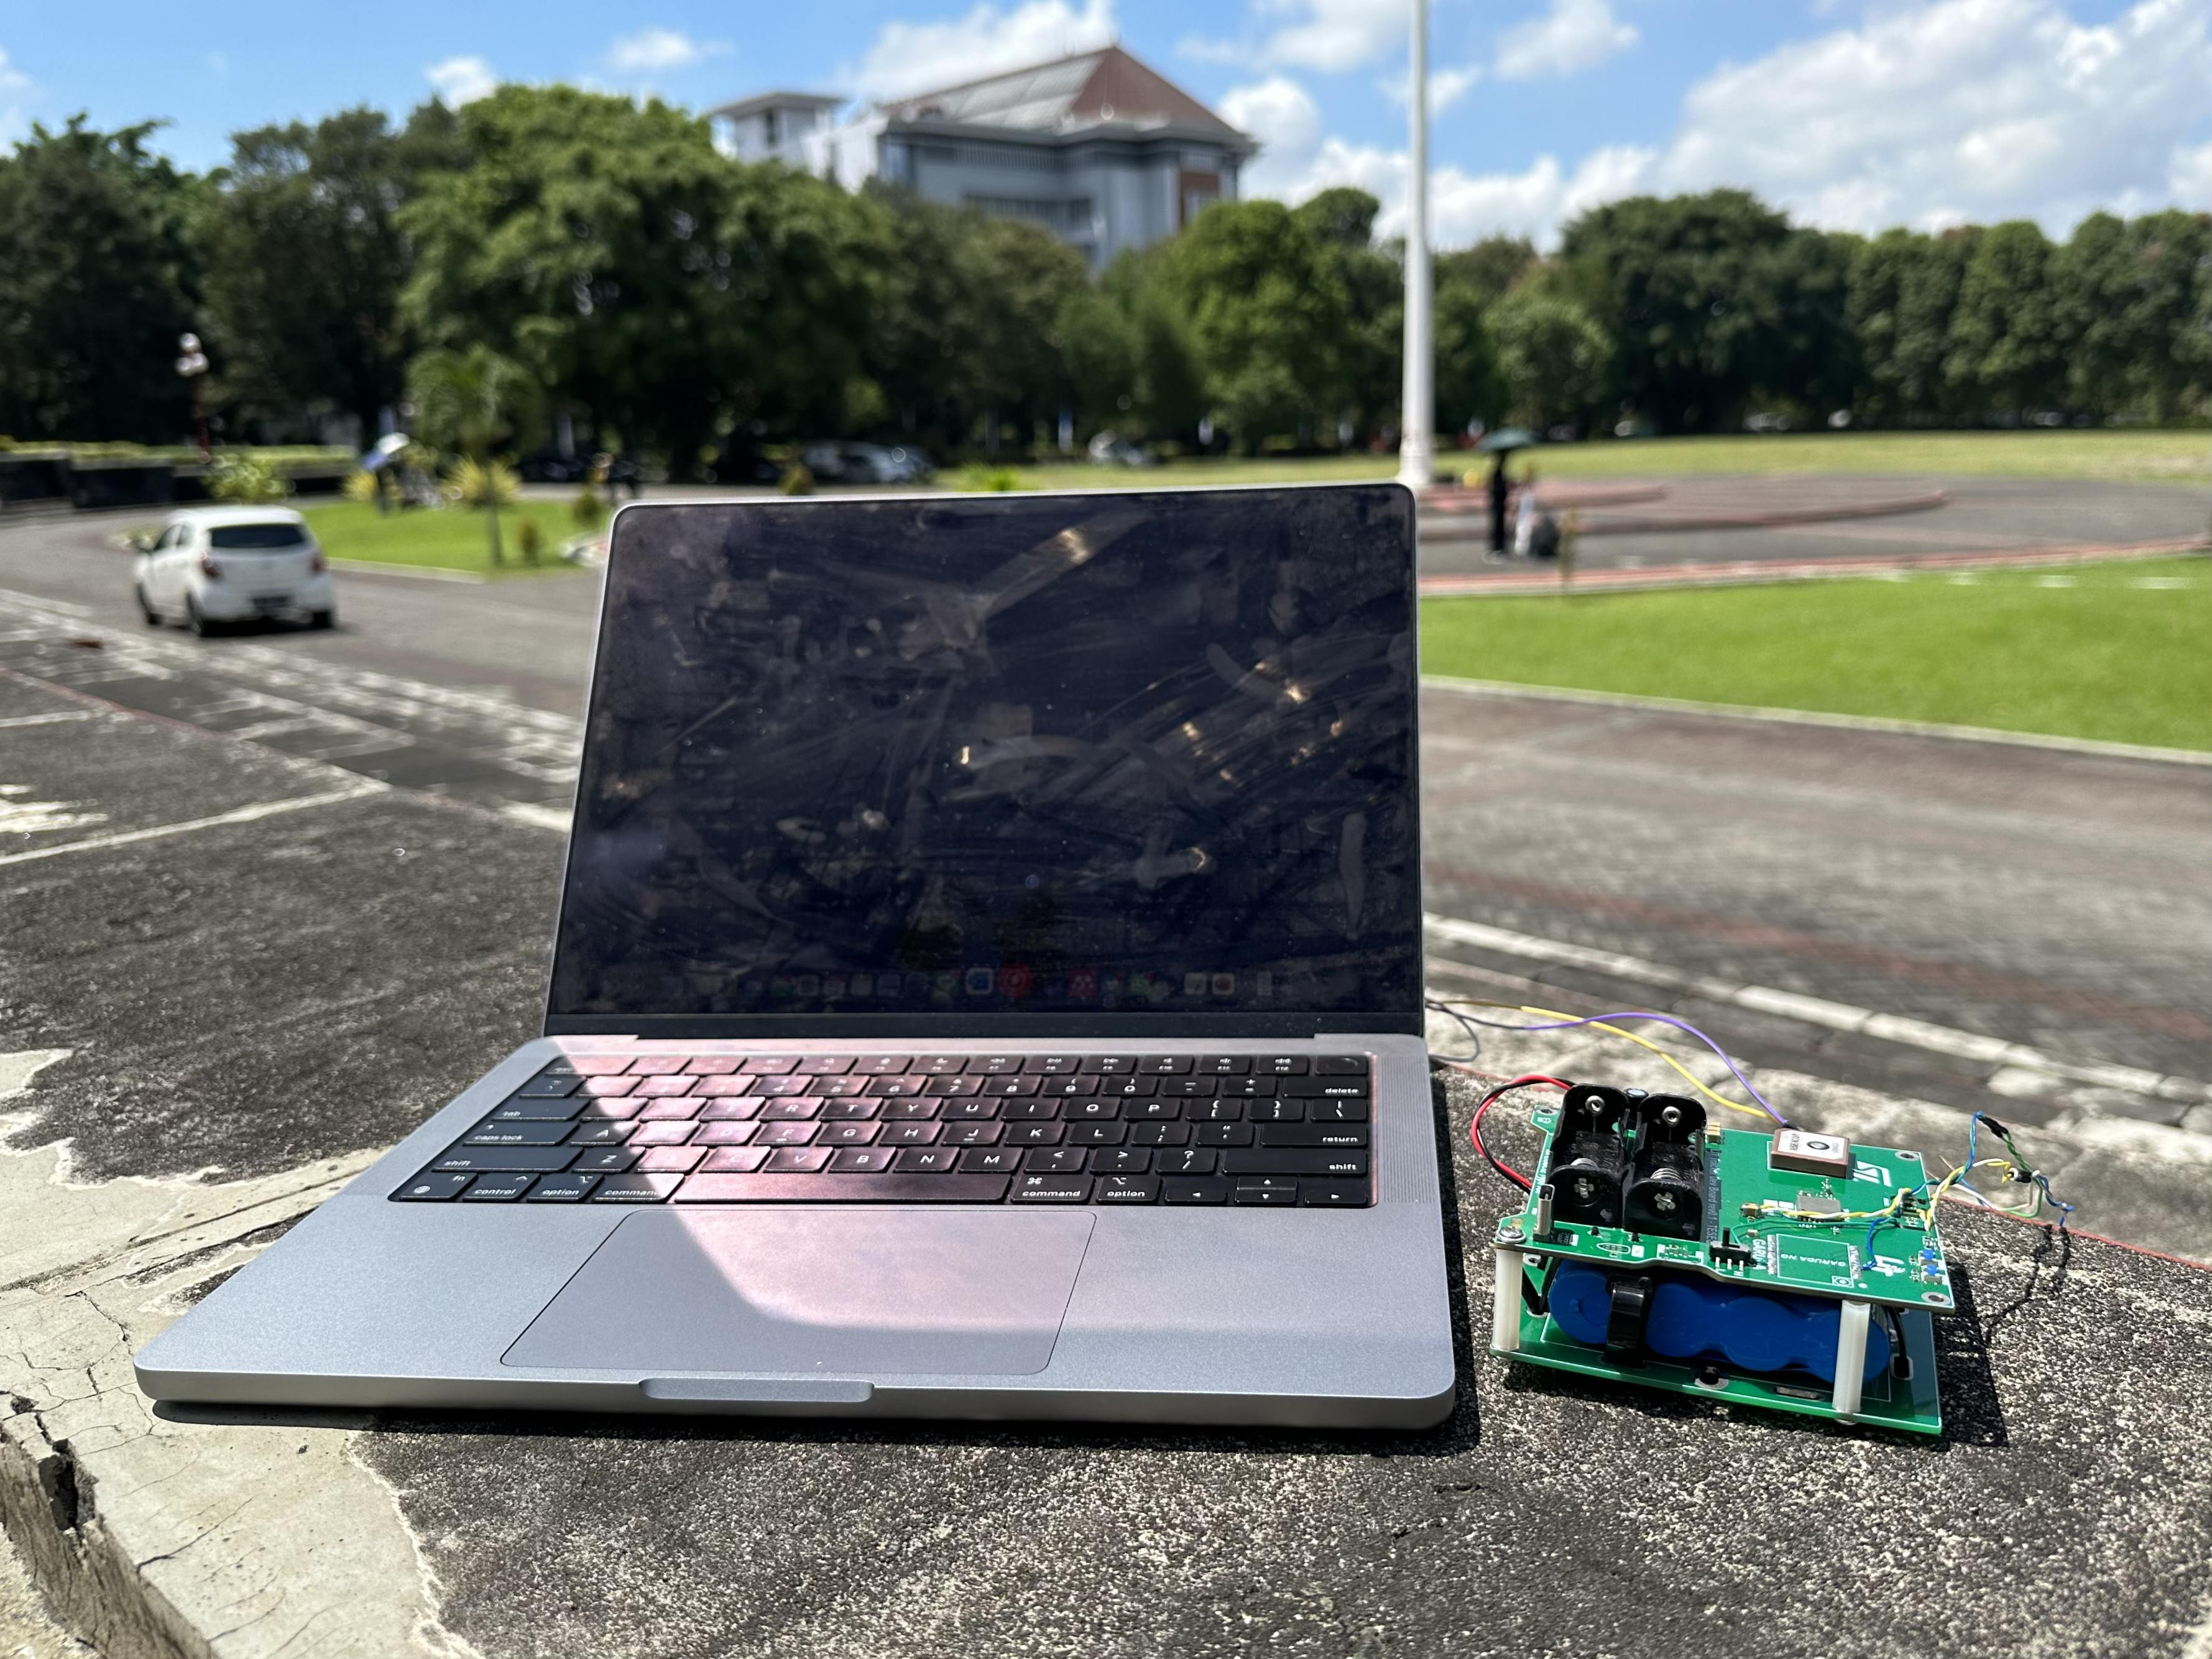
\includegraphics[width=10cm]{contents/chapter-4/4-skenario-outdoor/keadaan.jpg}
	\caption{Keadaan sekitar pengujian skenario ruang terbuka}
	\label{Fig: outdoor-keadaan}
\end{figure}

\subsection{Skenario Ruangan Terbuka}
Pengujian skenario ruangan terbuka bertujuan untuk meninjau performa modul Teseo\hyp{}LIV3FL di ruangan terbuka. Titik pengujian berada di Lapangan Pancasila Universitas Gadjah Mada dengan kondisi langit cerah. Pemilihan lokasi Lapangan Pancasila bertujuan untuk meminimalisasi penghalang seperti gedung dan pepohonan. Gambar \ref{Fig: outdoor-keadaan} menunjukan pengujian skenasio ruangan terbuka. Berdasarkan penelitian \cite{Lu2018}, lingkungan dengan penghalang paling sedikit seperti skenario ruangan terbuka dapat meningkatkan ketelitian dan kepresisian dari modul GNSS.

\begin{figure}[H]
	\centering
	\begin{adjustbox}{width=\textwidth}
		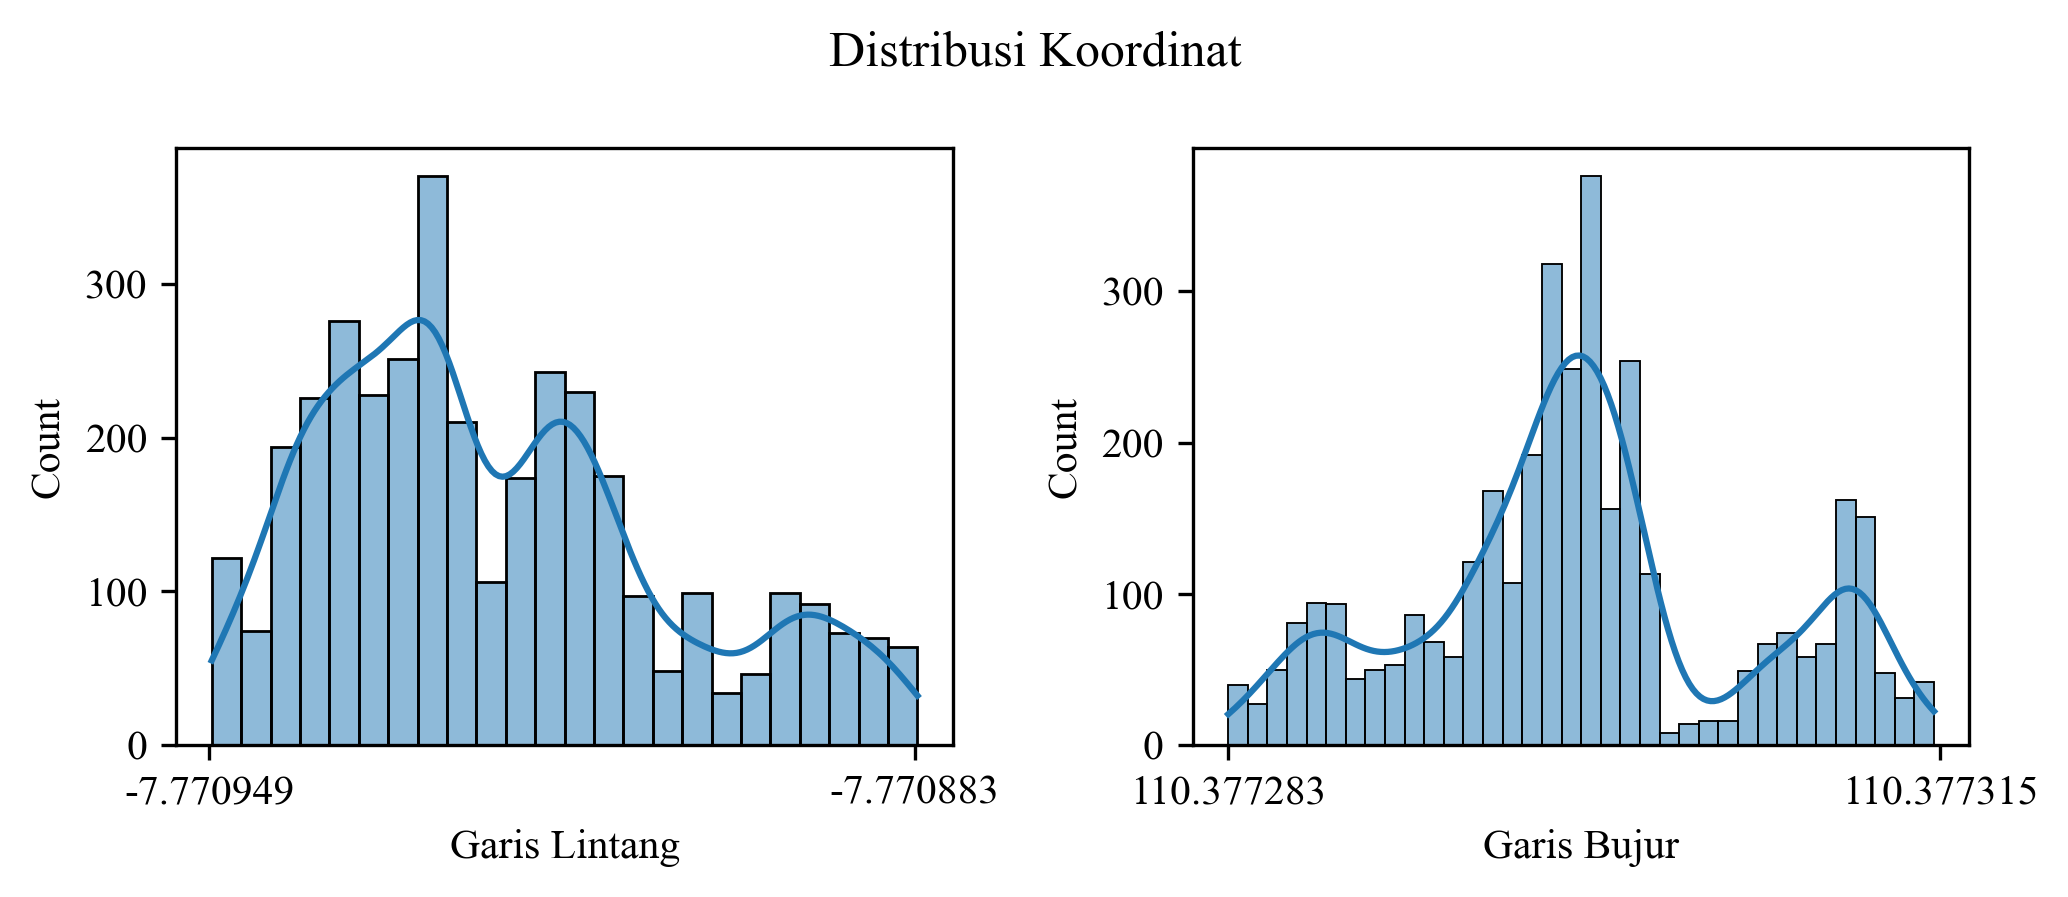
\includegraphics{contents/chapter-4/4-skenario-outdoor/distribution.png}
	\end{adjustbox}
	\caption{Distribusi data koordinat skenario ruang terbuka}
	\label{Fig:outdoor-distribution}
\end{figure}

Distribusi koordinat hasil pengujian luar ruangan ditunjukan oleh Gambar \ref{Fig:outdoor-distribution}. Koordinat garis lintang berada pada rentang -7,770949 hingga -7,770883, sedangkan koordinat garis bujur berada pada rentang 110,377283 hingga 110,377315. Sama seperti tiga pengujian sebelumnya, berdasarkan uji Shapiro-Wilk, koordinat pada hasil pengujian ruang terbuka tidak terdistribusi normal. Karena data koordinat tidak terdistribusi normal maka akan dilakukan analisis terhadap nilai MAD-nya juga.

\begin{table}[H]
	\caption{Hasil Pengujian Ruangan Terbuka}
	\vspace{0.5em}
	\centering
	\begin{tabular}{ccccc}
		\hline
		& \textbf{Minima} & \textbf{Maxima} & \textbf{Rata-rata} & \textbf{Standar Deviasi}\\
		\hline 
		HDOP & 0,60 & 0,80 & 0,65 & 0,06 \\
		PDOP & 0,90 & 1,60 & 1,12 & 0,15 \\
		VDOP & 1,10	& 1,80 & 1,30 & 0,15 \\
		CEP (m) & 5,22 & 6,80 & 6,12 & 0,41 \\
		Jumlah Satelit & 17	& 25 & 21,14 & 1,37 \\
		\hline
		\textbf{MAD-x (m)} & & \multicolumn{2}{c}{\centering 0,94} & \\
		\hline
		\textbf{MAD-y (m)} & & \multicolumn{2}{c}{\centering 0,76} & \\
		\hline
		\textbf{MAD (m)} & & \multicolumn{2}{c}{\centering 1,21} & \\
		\hline
	\end{tabular}
	\label{Tab: outdoor-table}
\end{table}

\begin{figure}[H]
	\centering
	\includegraphics[width=12cm]{contents/chapter-4/4-skenario-outdoor/sky_plot.png}
	\caption{\textit{Sky plot} pengujian ruang terbuka}
	\label{Fig: outdoor-skyplot}
\end{figure}

Tabel \ref{Tab: outdoor-table} menunjukan bahwa pada skenario ruang terbuka memberikan hasil akurasi yang lebih tinggi. Rata-rata nilai DOP yang didapat berada pada rentang sangat baik sampai dengan ideal. Rata-rata nilai PDOP yang didapat adalah sebesar 1,12 dengan PDOP terkecil adalah 0,90 dan terbesarnya 1,60. Nilai PDOP yang kecil didukung oleh persebaran satelit di langit yang lebih banyak mencakup bagian lingkaran pada Gambar \ref{Fig: outdoor-skyplot}. Tingkat kepresisian pada skenario ini ditunjukan oleh nilai MAD-nya, yaitu 0,94 meter untuk koordinat garis lintang, 0,76 meter pada garis bujur, dan 1,21 meter untuk keseluruhannya.

\begin{figure}[H]
	\centering
	\includegraphics[width=13cm]{contents/chapter-4/4-skenario-outdoor/cep.png}
	\caption{CEP pengujian skenario ruang terbuka}
	\label{Fig: outdoor-cep}
\end{figure}

Nilai CEP yang didapat pada pengujian ini adalah nilai CEP terbaik dari tiga skenario sebelumnya. Tren nilai CEP cenderung stabil dan tidak ada lonjakan yang signifikan seperti ditunjukan oleh Gambar \ref{Fig: outdoor-cep}. Hal tersebut sejalan dengan nilai standar deviasinya yang sangat rendah. Pada pengujian ini, nilai CEP dapat menyentuh nilai 5,22 meter dan paling tinggi sebesar 6,80 meter. Meskipun masih lebih tinggi dari \textit{datasheet} (1,50 meter), nilai tersebut sudah cukup untuk aplikasi pelacak bus Trans Gadjah Mada.

\begin{figure}[H]
	\centering
	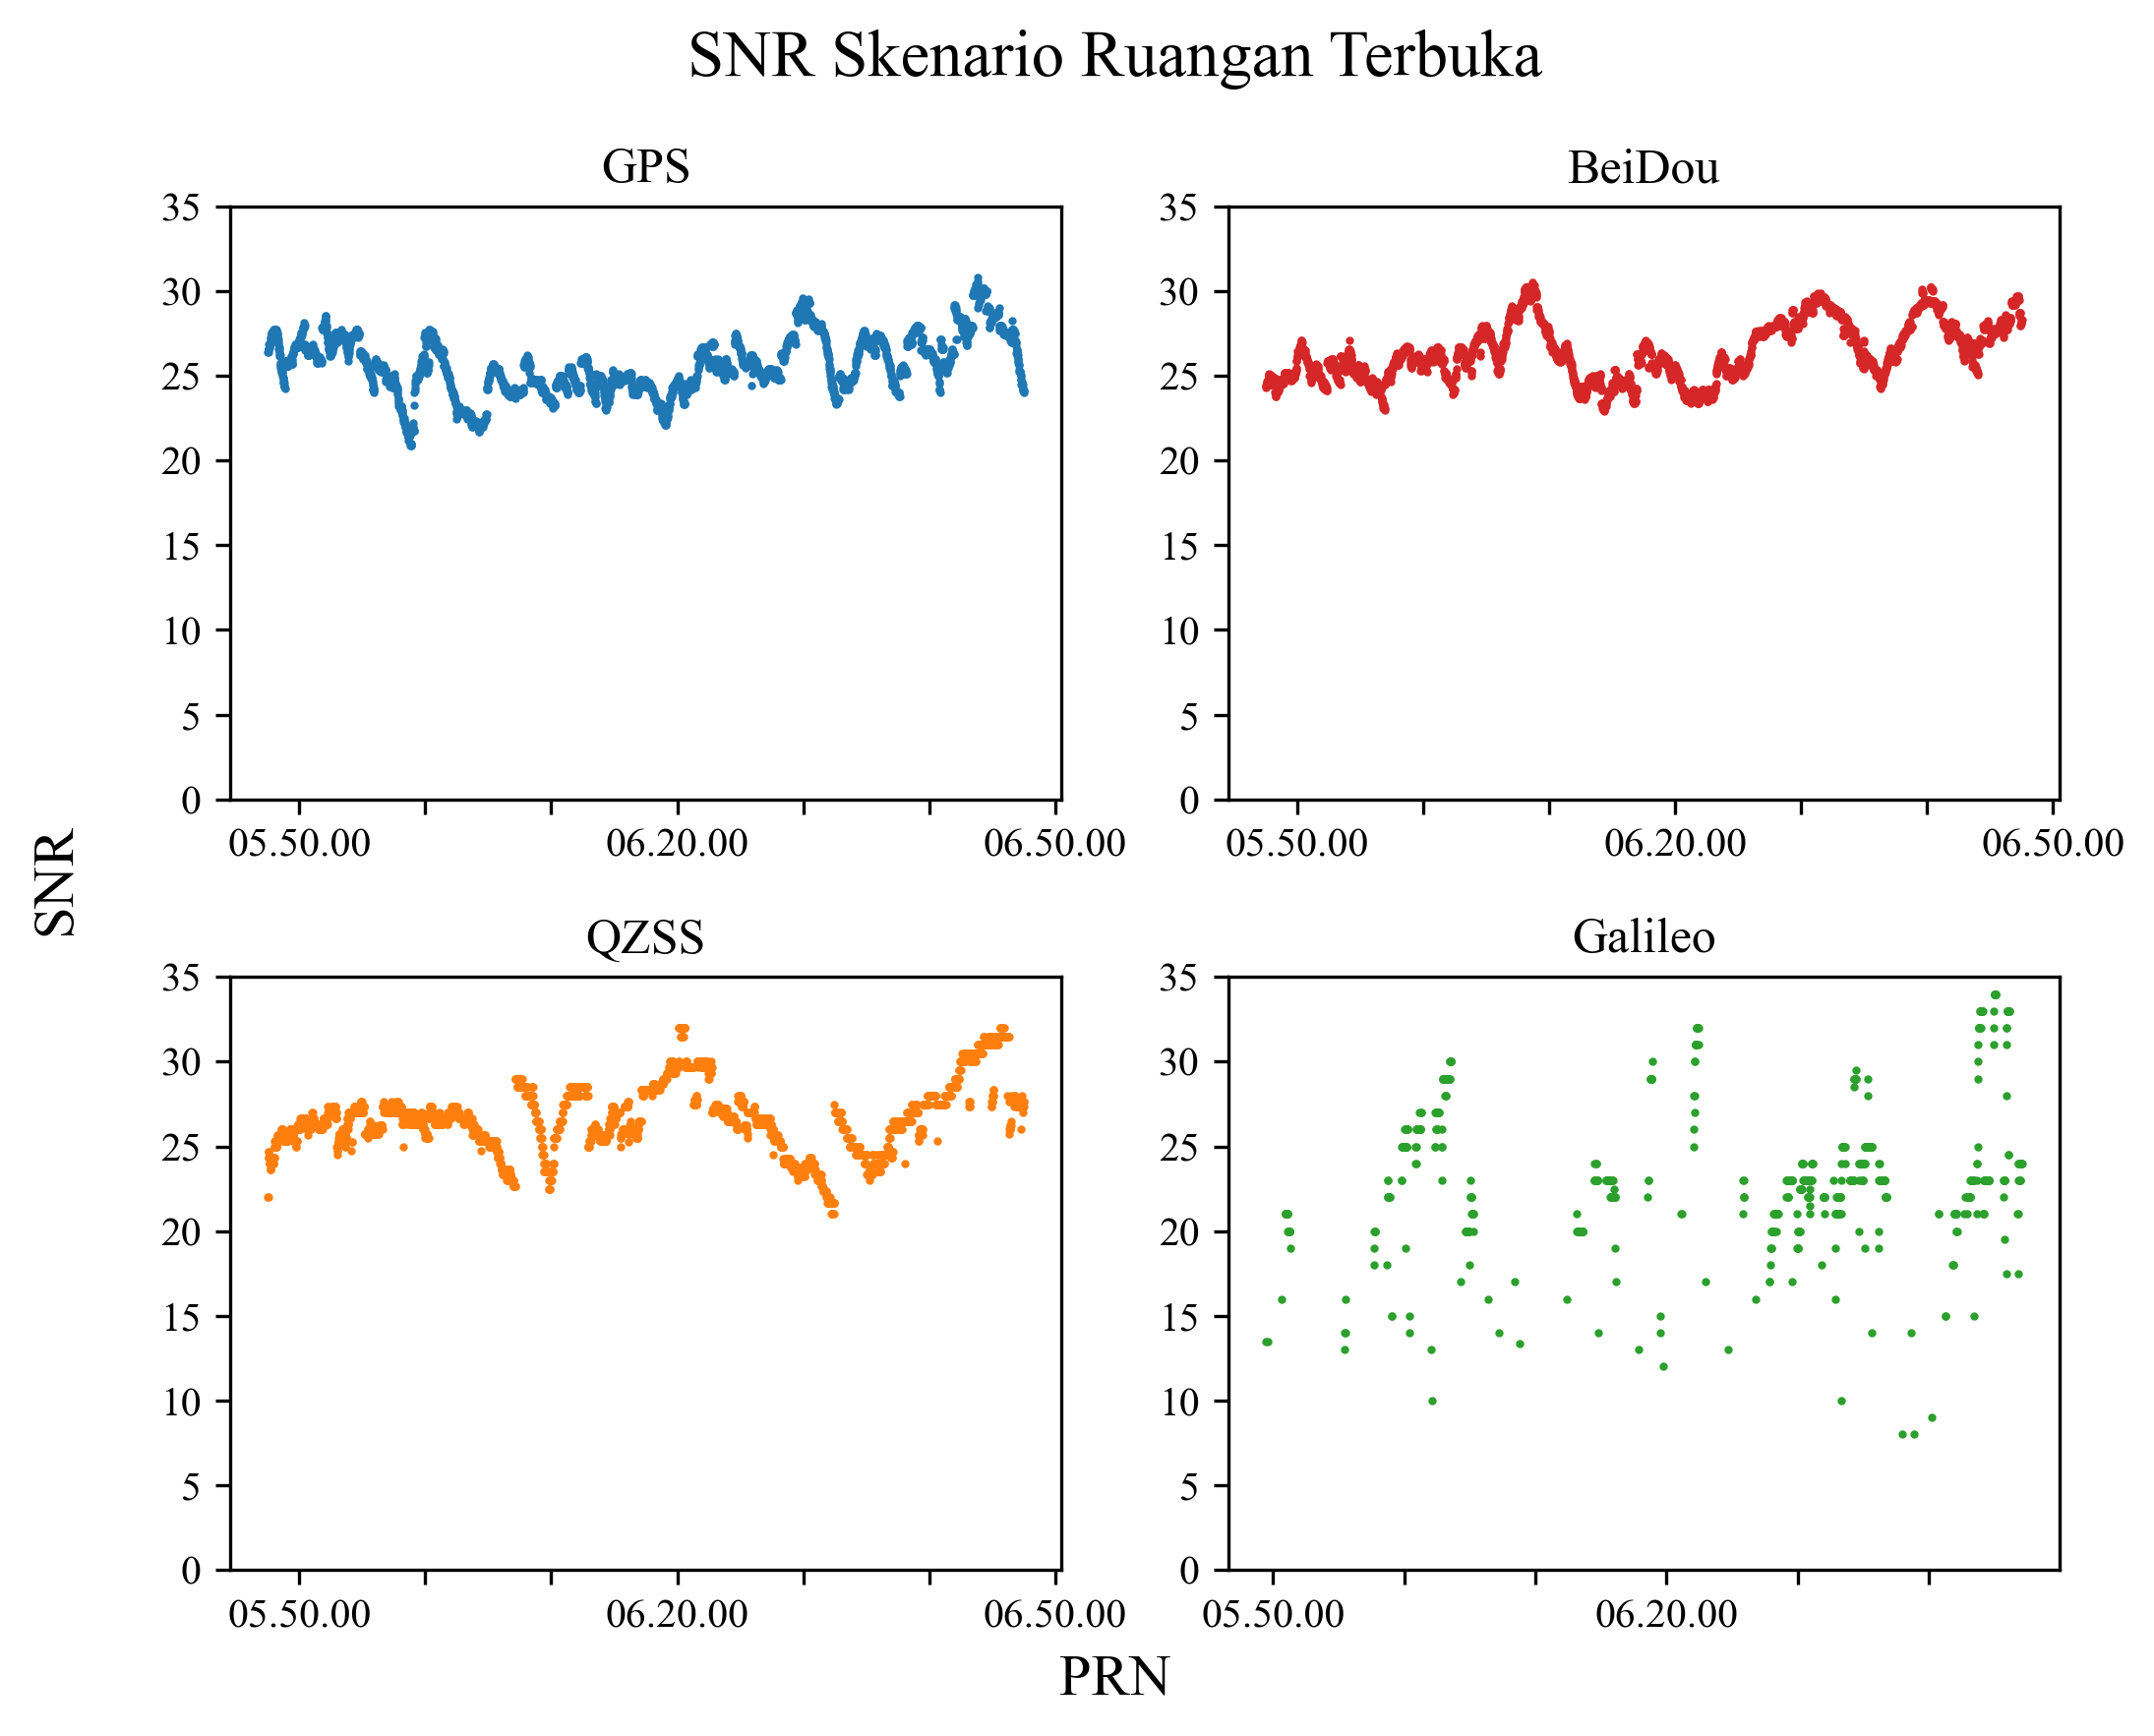
\includegraphics[width=13cm]{contents/chapter-4/4-skenario-outdoor/snr.png}
	\caption{SNR setiap konstelasi pada pengujian skenario ruang terbuka}
	\label{Fig: outdoor-snr}
\end{figure}

Jika meninjau nilai SNR-nya, terlihat bahwa nilai SNR pada skenario ini tidak berbeda jauh dengan skenario ruangan semi-terbuka. Seperti ditunjukan oleh Gambar \ref{Fig: outdoor-snr}, nilai SNR dari seluruh konstelasi mengalami peningkatan yang cukup signifikan, yaitu mencapai 5 dB. Jumlah data SNR pada konstelasi Galileo tidak berbeda jauh dengan skenario ruangan semi-terbuka, tetapi terjadi peningkatan terhadap nilai SNR terkecilnya, yaitu 10 dB. Selain itu, peningkatan visibilitas satelit yang sangat signifikan juga mempengaruhi nilai CEP pada skenario ini. 

\begin{figure}[H]
	\centering
	\begin{adjustbox}{width=\textwidth}
		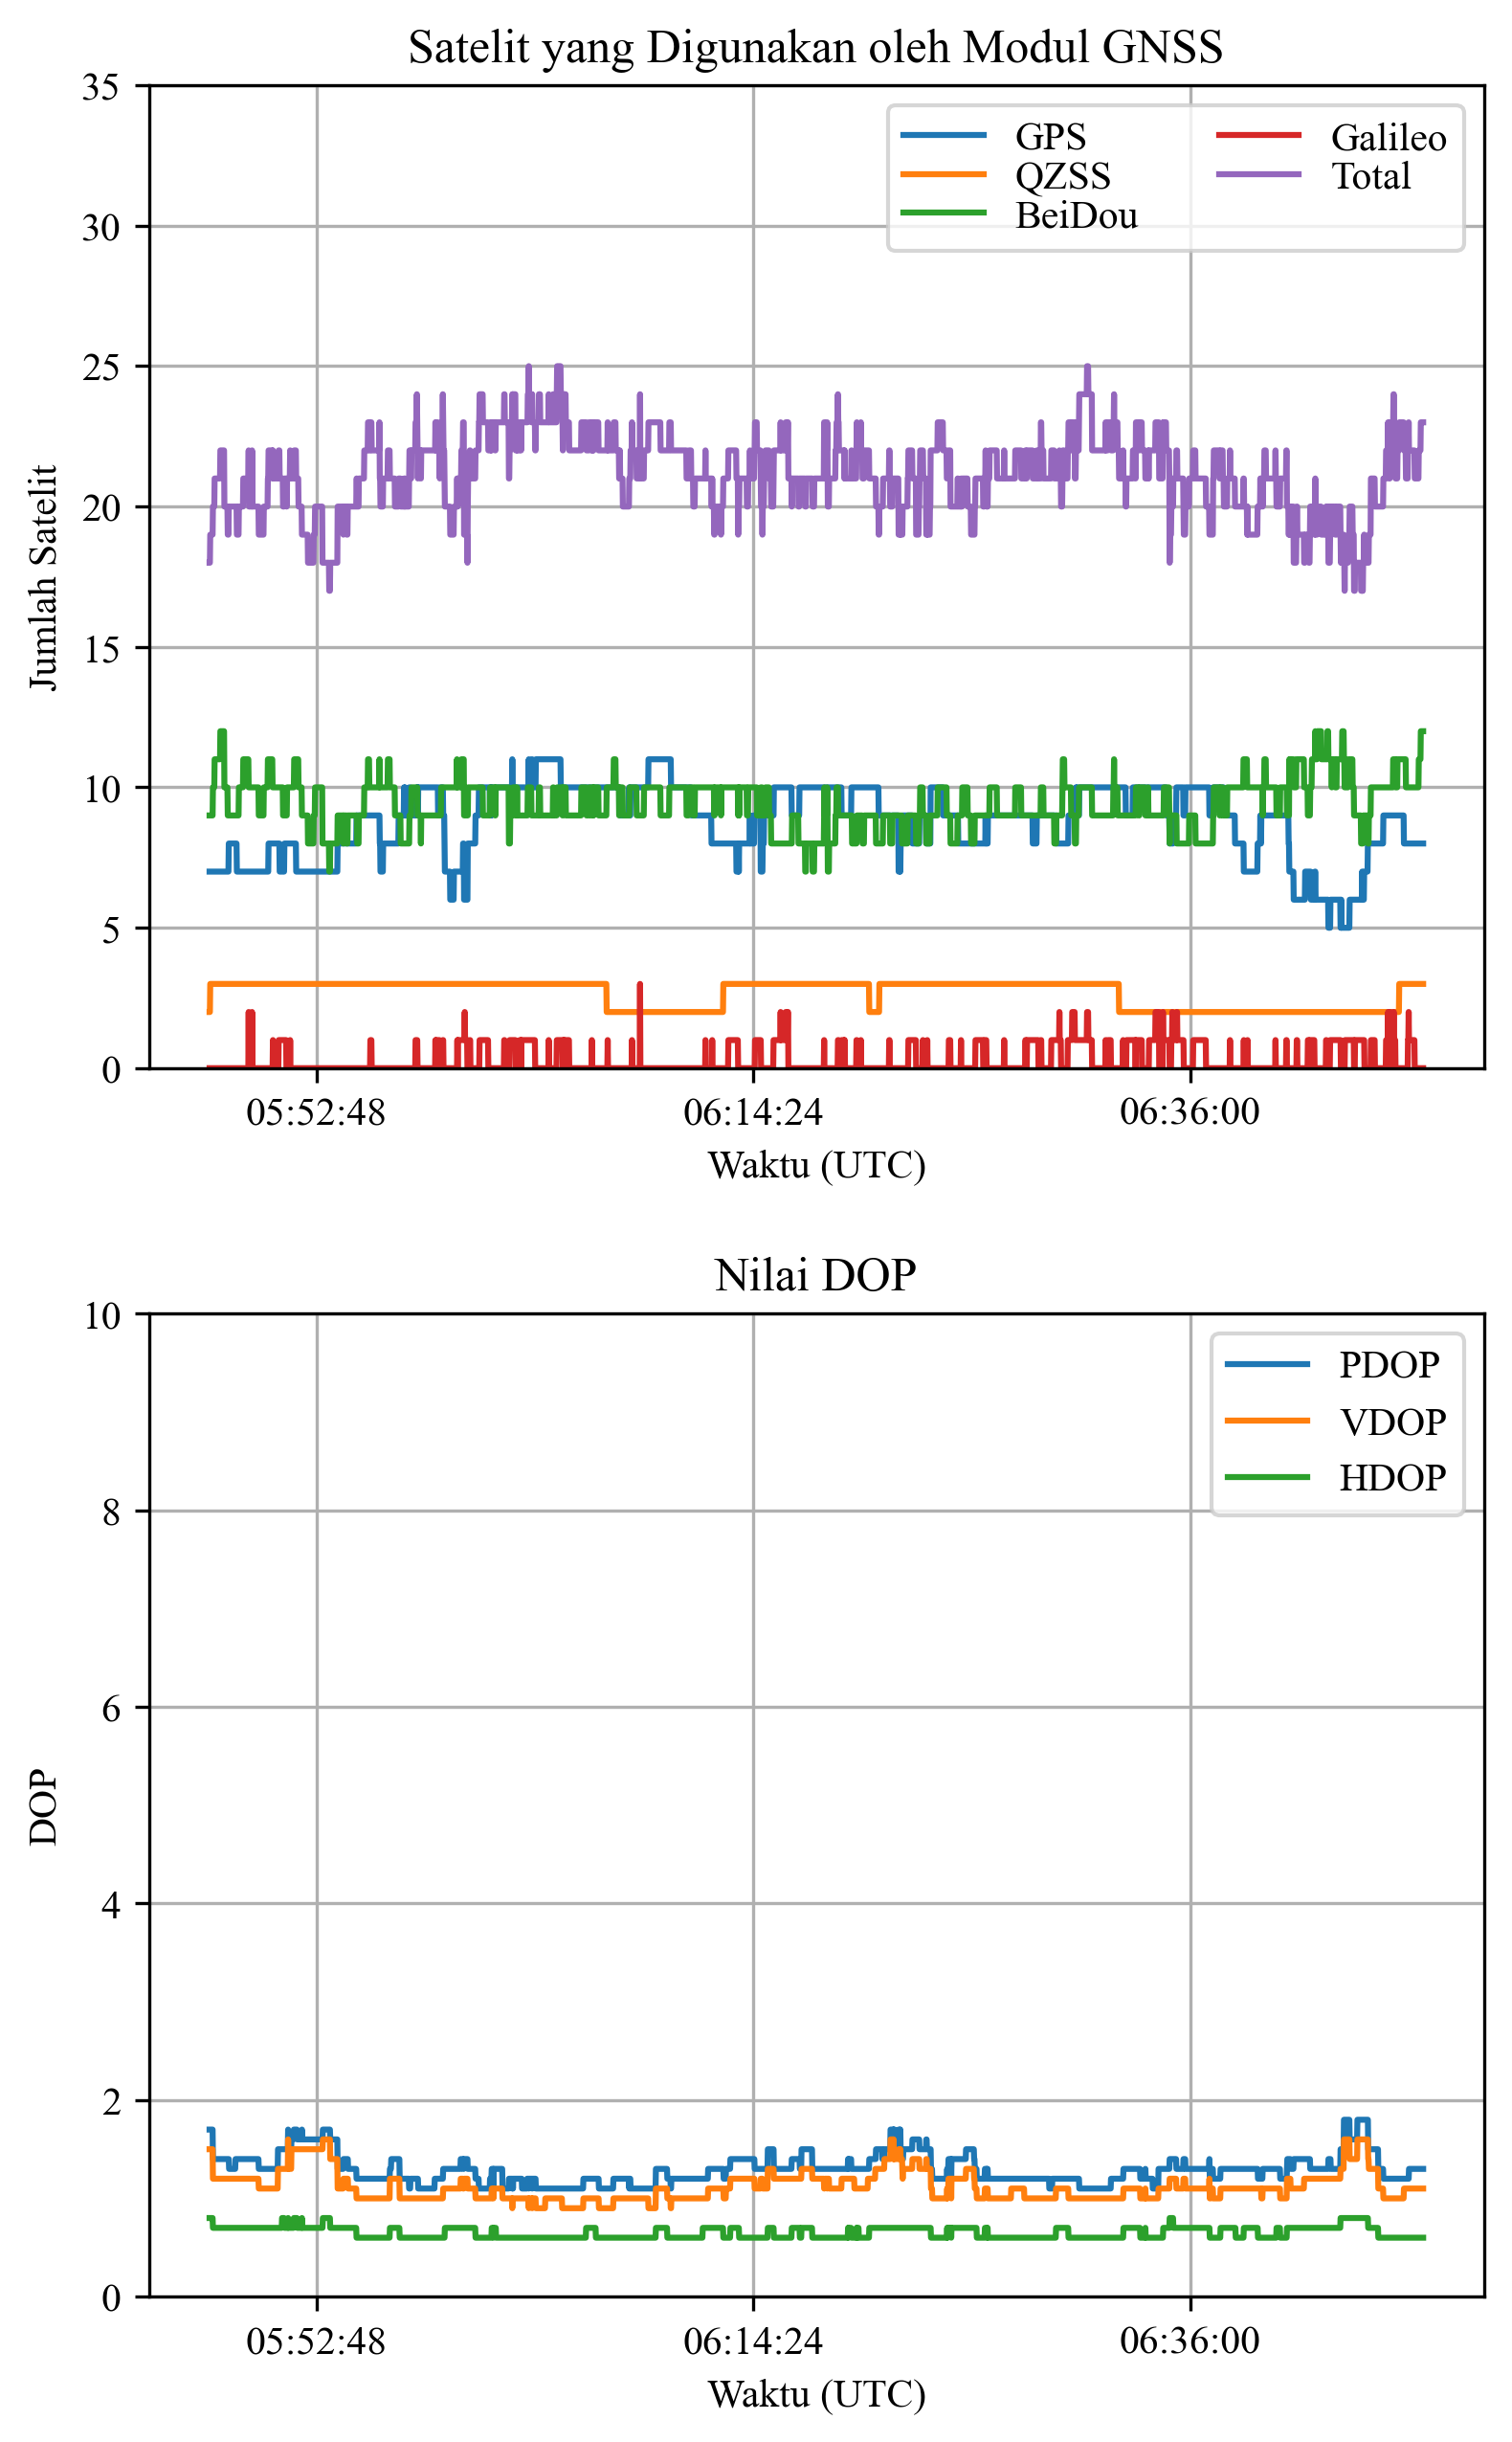
\includegraphics{contents/chapter-4/4-skenario-outdoor/sats_dop.png}
	\end{adjustbox}
	\caption{DOP dan visibilitas satelit pengujian ruang terbuka}
	\label{Fig: outdoor-dop_sats}
\end{figure}

Gambar \ref{Fig: outdoor-dop_sats} menunjukan tren ketiga nilai DOP dan visibilitas satelit selama satu jam. Visibilitas satelit terkecil adalah 17 buah satelit dan paling banyak adalah dua puluh lima satelit. Konstelasi GPS dan BeiDou masih menjadi konstelasi paling dominan, diikuti oleh konstelasi QZSS dengan visibilitas satelit stabil di antara dua sampai dengan lima satelit. Sementara itu, visibilitas satelit pada konstelasi Galileo bervariasi antara nol hingga dua satelit saja. Terdapat sedikit lonjakan pada nilai DOP, tetapi lonjakan tersebut tidak terlalu signifikan karena masih berada dalam kategori sangat baik.

Hasil pengujian menunjukkan bahwa skenario pengujian di ruang terbuka menghasilkan hasil pengukuran yang paling baik dibandingkan dengan tiga pengujian sebelumnya. Dari pengujian tersebut, didapatkan nilai MAD sebesar 1,21 meter dan CEP rata-rata sebesar 6,12 meter. Jika dibandingkan dengan tiga skenario sebelumnya, skenario ruang terbuka menunjukkan hasil pengujian paling baik. Oleh karena itu, untuk mendapatkan hasil pengukuran terbaik maka modul Teseo\hyp{}LIV3FL harus diletakkan di ruangan terbuka.

\section{Pengujian \textit{Geofencing}}
\subsection{\textit{Geofencing} Wilayah Universitas Gadjah Mada}
Tujuan dari pengujian fitur \textit{geofencing} di wilayah Universitas Gadjah Mada adalah untuk meninjau apakah fitur ini dapat berfungsi dengan baik untuk menentukan status \textit{geofencing} pengguna saat ini. Dalam pengujian ini, wilayah \textit{geofencing} didefinisikan sebagai lingkaran dengan jari-jari satu kilo meter dengan pusat di titik (-7,771376; 110,377493) dan delapan belas titik acak di sekitar Universitas Gadjah Mada digunakan sebagai titik pengujian.

\begin{figure}[H]
	\centering
	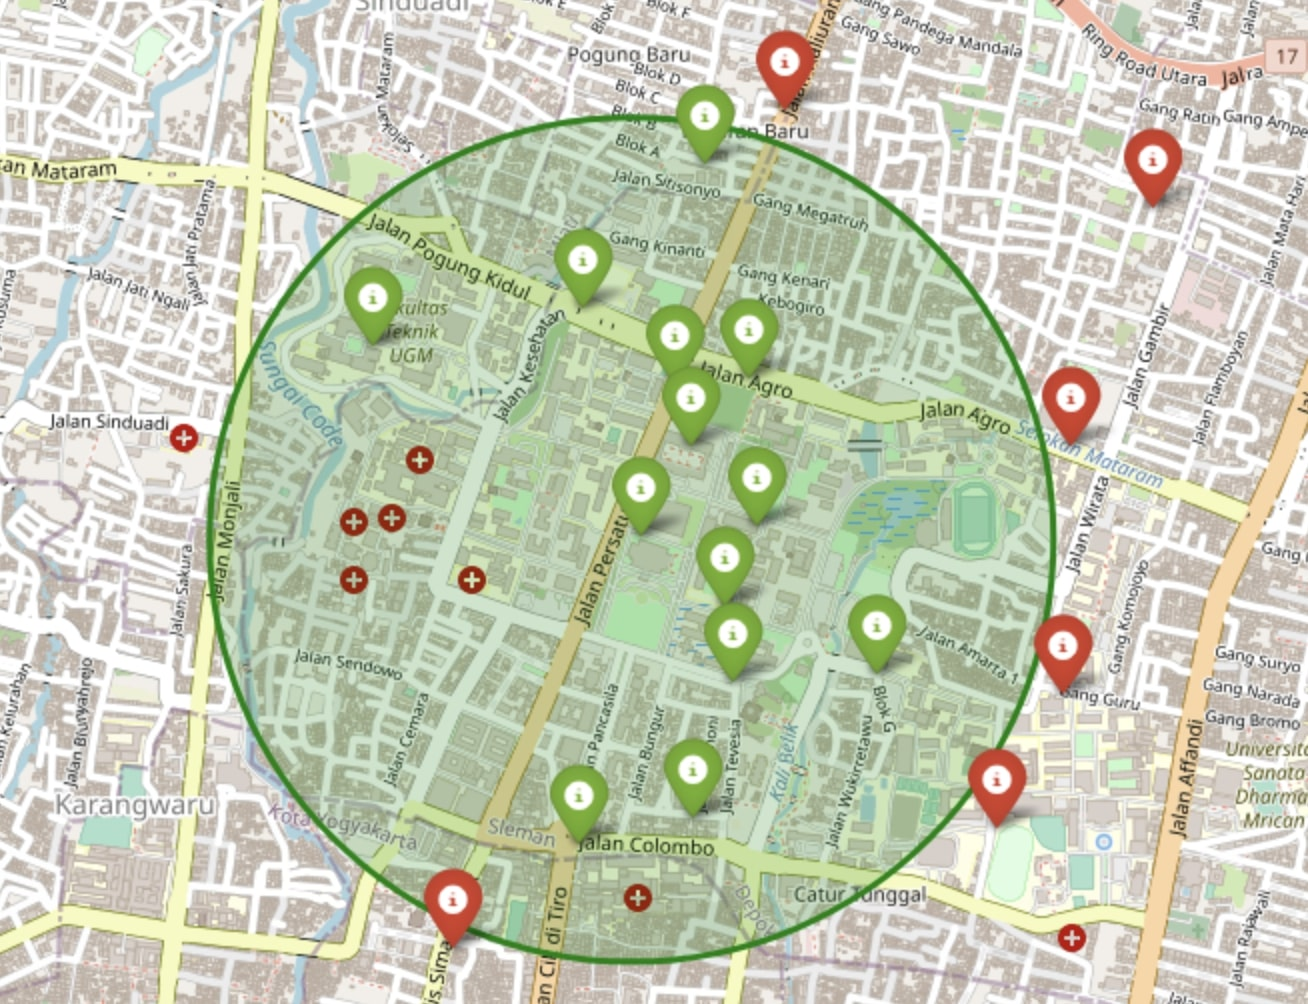
\includegraphics[width=10cm]{contents/chapter-4/geofencing/wilayah-ugm.jpg}
	\caption{Hasil Pengujian \textit{Geofencing} di Wilayah Universitas Gadjah Mada}
	\label{Fig: geofencing-1}
\end{figure}

Dalam pengujian ini, fitur \textit{geofencing} dijalankan pada setiap titik pengujian dan hasilnya dicatat. Hasil pengujian tersebut kemudian dianalisis untuk menentukan apakah hasil algoritma \textit{geofencing} pada \textit{firmware} sudah tepat atau belum. Gambar \ref{Fig: geofencing-1} menunjukkan hasil dari pengujian tersebut dengan wilayah \textit{geofencing} ditandai oleh lingkaran berwarna hijau. Simbol berwarna merah merepresentasikan jika \textit{firmware} mendeteksi bahwa posisi saat ini berada di luar wilayah \textit{geofencing} dan sebaliknya untuk simbol berwarna hijau.

Dari hasil pengujian, terlihat bahwa seluruh titik di luar lingkaran hijau ditunjukkan oleh simbol berwarna merah, dan titik berwarna hijau untuk kondisi sebaliknya. Hal ini menunjukkan bahwa fitur \textit{geofencing} di wilayah Universitas Gadjah Mada sudah berjalan dengan baik dan mampu mendeteksi status \textit{geofencing} bus di wilayah Universitas Gadjah Mada dengan baik.

\begin{table}[H]
	\caption{Koordinat Halte Pengujian \textit{Geofencing} Halte}
	\vspace{0.5em}
	\centering
	\begin{tabular}{cc}
		\hline
		\textbf{Halte} &\textbf{Koordinat} \\
		\hline
		6 & -7,769693; 110,373557 \\
		8 &-7,766077; 110,374062\\ 
		11 &-7,766508; 110,3706700\\
		13 & -7,766407; 110,3740824\\
		17 &-7,769712; 110,385479\\ 
		20 & -7,771089; 110,381336\\
		21 & -7,772668; 110,379638\\
		\hline
	\end{tabular}
	\label{Tab: geofencing-2}
\end{table}

\subsection{\textit{Geofencing} Halte}
Pengujian fitur \textit{geofencing} pada setiap halte bertujuan untuk meninjau apakah fitur \textit{geofencing} untuk mendeteksi halte saat ini sudah berjalan dengan baik. Pengujian ini dilakukan pada tujuh dari dua puluh empat halte yang akan disinggahi oleh bus Trans Gadjah Mada. Setiap wilayah \textit{geofencing} halte memiliki jari-jari sebesar sepuluh meter. Tabel \ref{Tab: geofencing-2} menunjukan koordinat dari tujuh halte yang dijadikan sampel pada pengujian ini.

\begin{table}[H]
	\caption{Hasil Pengujian \textit{Geofencing} Halte Bus Trans Gadjah Mada}
	\vspace{0.5em}
	\centering
	\begin{tabular}{ccc}
		\hline
		\textbf{Koordinat} &\textbf{Halte pada \textit{Firmware}} & \textbf{Halte Aktual}\\
		\hline 
		-7,769638; 110,373497 & 6 & 6 \\
		-7,766024; 110,374046 & 8 & 8 \\
		-7,766489; 110,370709 & 11 & 11 \\
		-7,766449; 110,374107 & 13 & 13 \\
		-7,769756; 110,385509 & 17 & 17 \\
		-7,771065; 110,381348 & 20 & 20 \\
		-7,772746; 110,379647 & 21 & 21 \\
		\hline
	\end{tabular}
	\label{Tab: geofencing-3}
\end{table}

Fitur \textit{geofencing} akan diuji di keenam halte pengujian dan kemudian hasilnya dicatat. Pengujian dilakukan dengan meletakan sistem di dalam wilayah \textit{geofencing} setiap halte uji. Hasil pengujian \textit{geofencing} pada halte uji ditunjukan oleh Tabel \ref{Tab: geofencing-3}. Dapat dilihat bahwa \textit{firmware} sudah bisa memprediksi halte tempat bus berhenti saat ini. Bahkan, \textit{firmware} dapat memprediksi lokasi halte saat ini dengan tepat meskipun wilayah \textit{geofencing}-nya berdekatan seperti pada halte ke-13 dengan halte ke-8.

\begin{figure}[H]
	\centering
	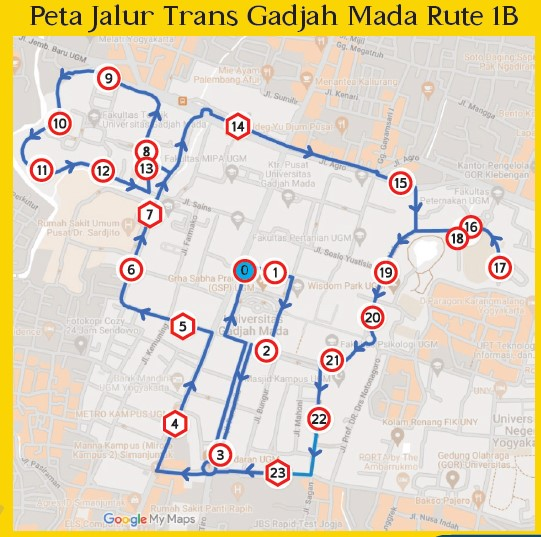
\includegraphics[width=8.5cm]{contents/chapter-4/pengujian-bergerak/Peta-Jalur-Rute-1B.jpg}
	\caption{Peta jalur Trans Gadjah Mada rute 1B}
	\label{Fig: peta-1b}
\end{figure}

\section{Pengujian di Bus Trans Gadjah Mada}
Pengujian secara langsung di bus Trans Gadjah Mada bertujuan untuk meninjau performa \textit{firmware} dalam keadaan bergerak. Dalam pengujian ini, sistem dipasang di dalam kendaraan bus listrik yang terbuat dari logam. Rute pengujian mengikuti rute 1B Trans Gadjah Mada yang dimulai dari Halte Grha Sabha Pramana hingga kembali lagi ke Halte Grha Sabha Pramana dengan durasi waktu satu jam.

Pada pengujian ini akan dibahas pada tiga hal, yaitu perbandingan hasil pelacakan dengan rute yang telah diberikan pada Gambar \ref{Fig: peta-1b}, hubungan HDOP dengan visibilitas satelit, dan analisis korelasi setiap variabelnya. Hasil pelacakan mencakup hasil pengukuran sistem dalam mengidentifikasi lokasi kendaraan. Hubungan HDOP dengan visibilitas satelit dibahas untuk meninjau performa sistem di bawah kondisi yang berbeda-beda. Analisis korelasi akan dilakukan untuk mengetahui keterkaitan antara parameter yang diperoleh oleh sistem.

\begin{figure}[H]
	\centering
	\begin{adjustbox}{width=\textwidth}
		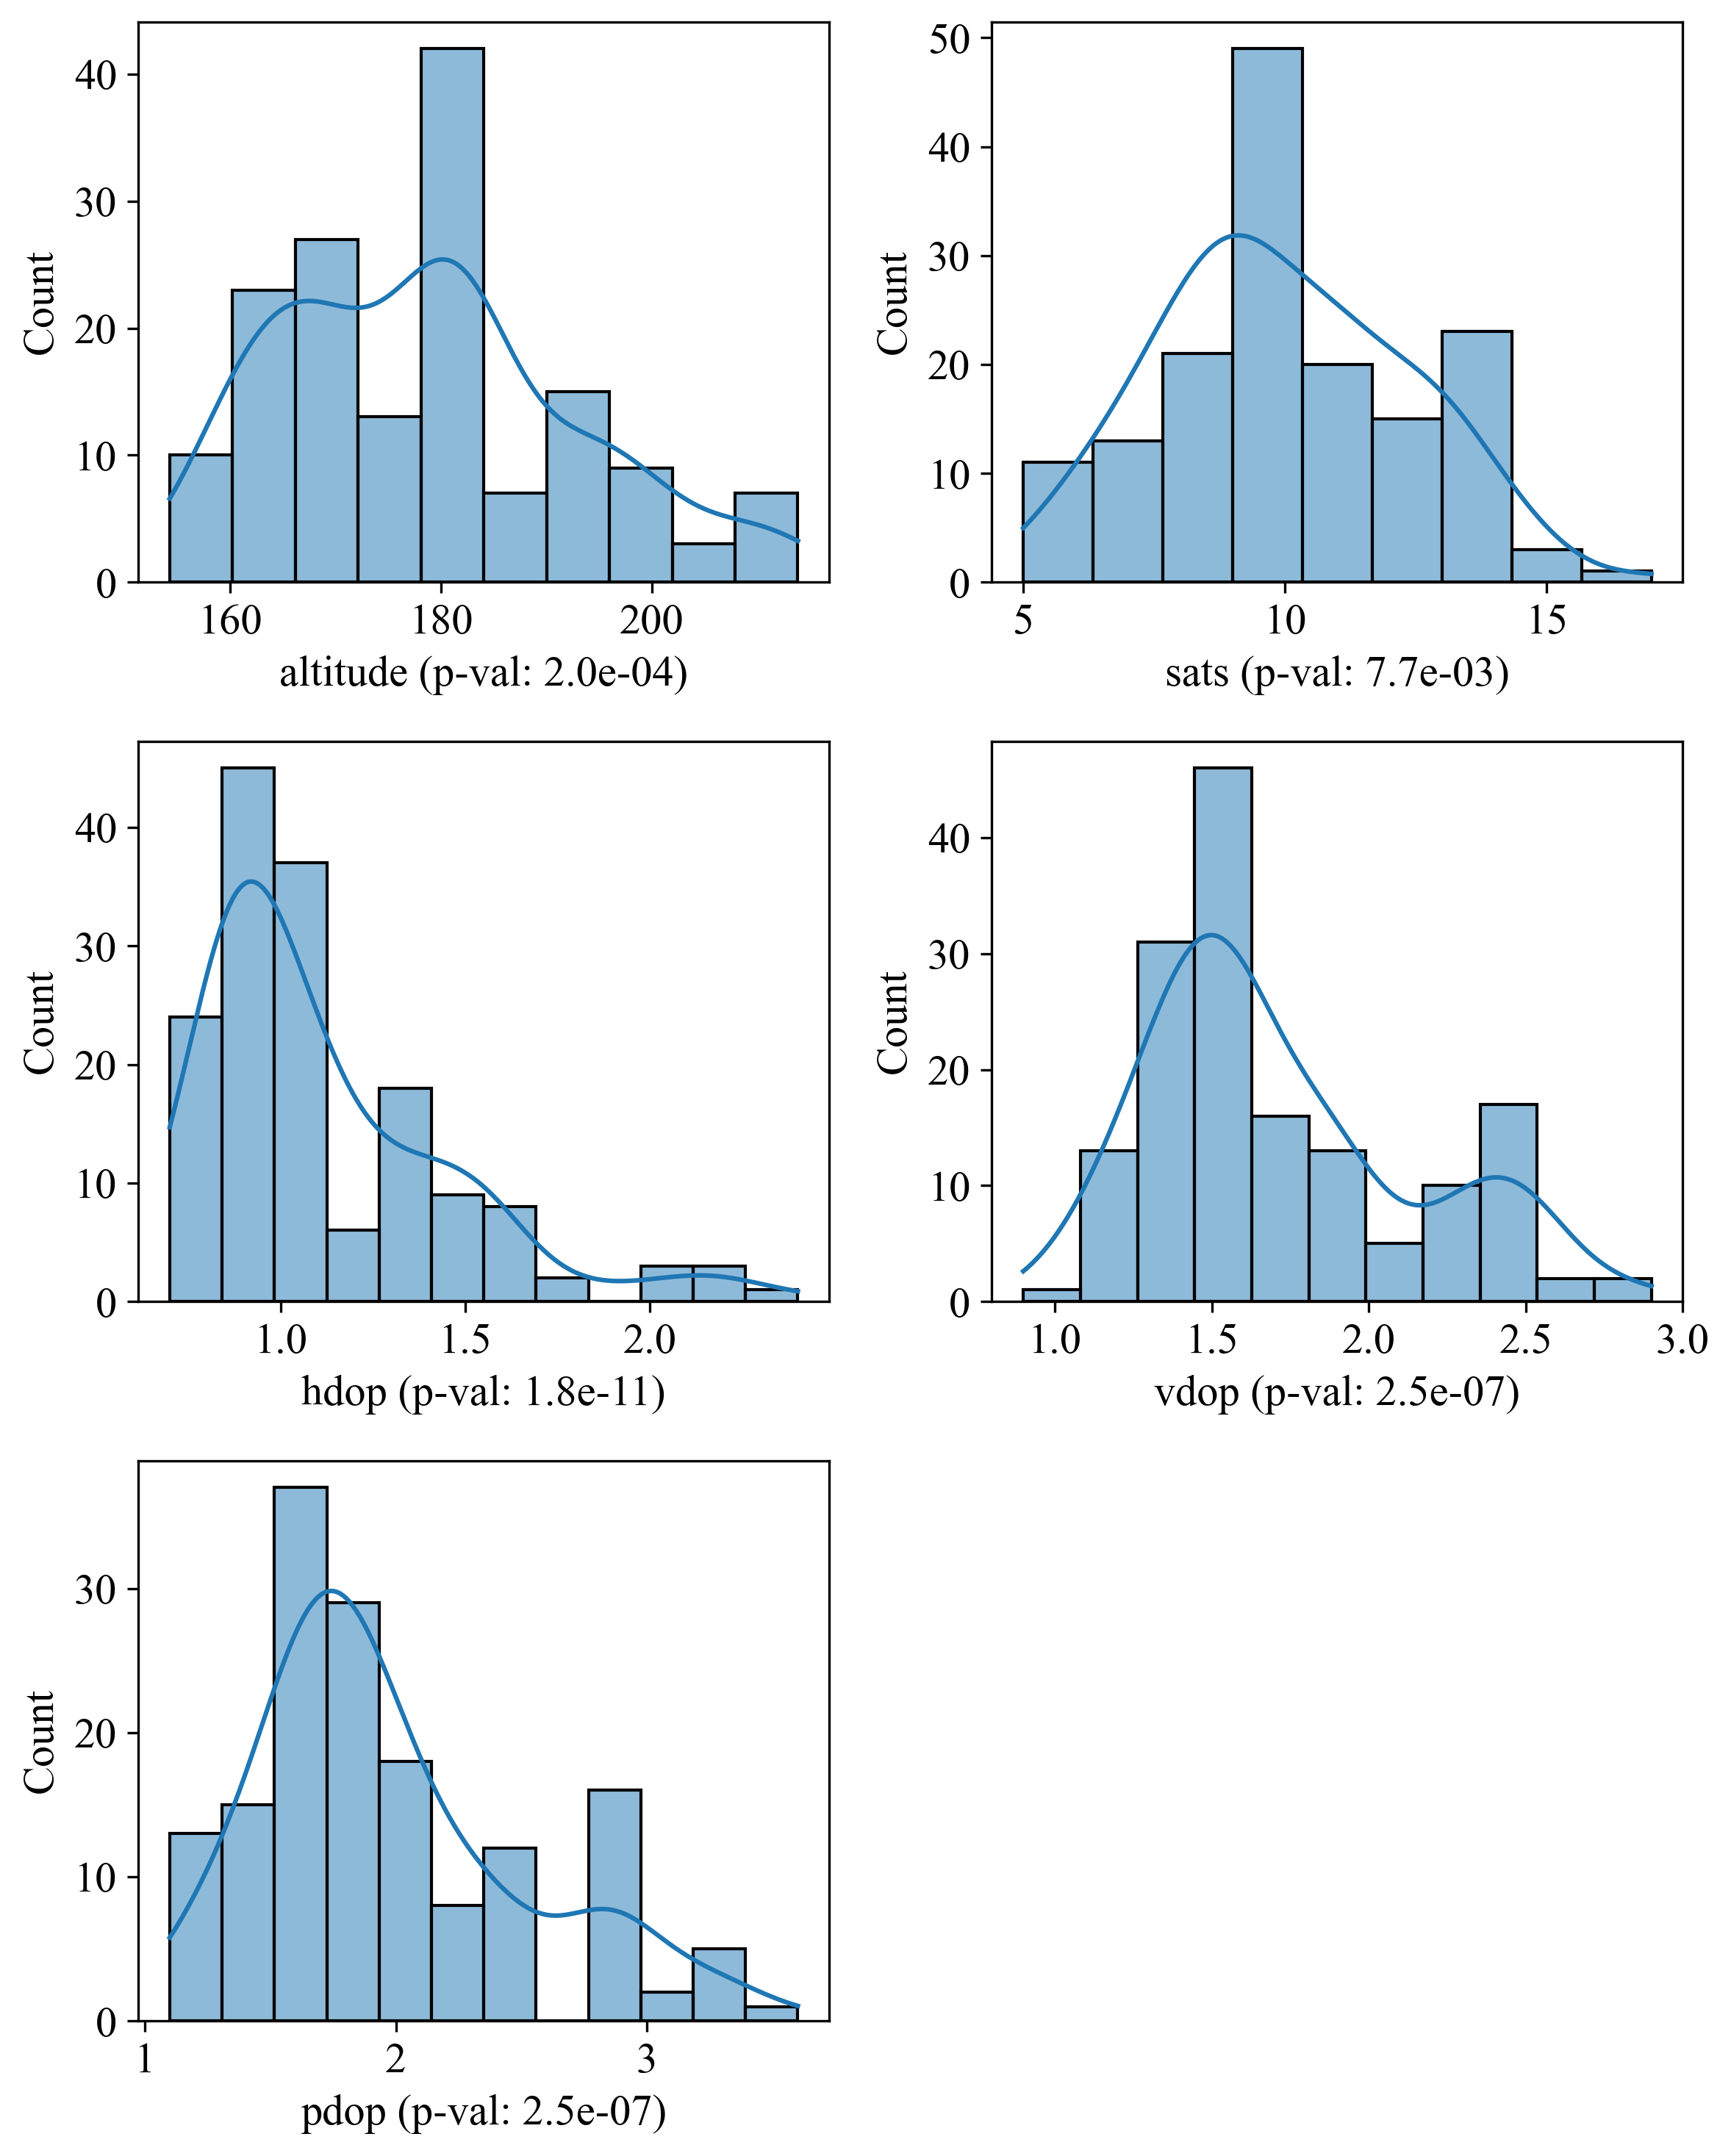
\includegraphics{contents/chapter-4/pengujian-bergerak/distribusi.png}
	\end{adjustbox}
	\caption{Distribusi setiap parameter pengujian bus Trans Gadjah Mada}
	\label{Fig: moving-distribusi}
\end{figure}

\subsection{Ikhtisar Data Hasil Pengujian}
Data hasil pengujian yang didapat terdiri dari delapan buah parameter, yaitu waktu, koordinat garis lintang dan garis bujur, visibilitas satelit, ketinggian, HDOP, dan status \textit{geofencing} saat ini. Pengambilan data dilakukan setiap dua puluh detik sekali sehingga didapat seratus enam puluh lima baris data. Selanjutnya, dilakukan uji statistik Saphiro-Wilk terhadap seluruh parameter, kecuali waktu dan status \textit{geofencing} saat ini dan hasilnya menunjukkan bahwa nilai $p$ dari seluruh parameter tersebut bernilai kurang dari 0,05. Hal ini menunjukkan bahwa seluruh parameter tersebut tidak terdistribusi secara normal. Selain itu, dapat dilihat pada Gambar \ref{Fig: moving-distribusi} bahwa setiap parameter terdistribusi dengan berbagai macam pola distribusi yang berbeda-beda.

\begin{figure}[H]
	\centering
	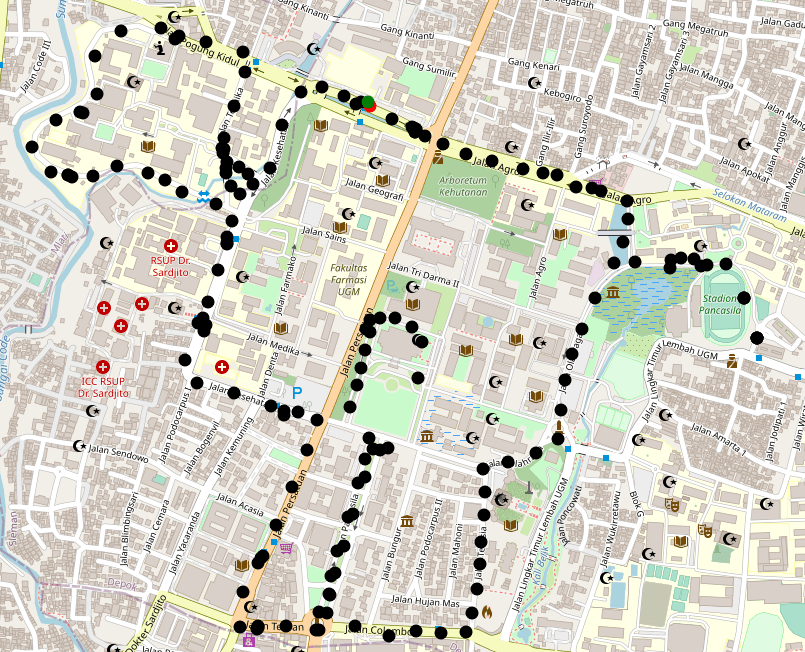
\includegraphics[width=12cm]{contents/chapter-4/pengujian-bergerak/tracked-route.png}
	\caption{Hasil pelacakan Bus Trans Gadjah Mada}
	\label{Fig: moving-tracked-route}
\end{figure}

Setelah itu, parameter koordinat garis lintang dan garis bujur akan di-\textit{plot} pada peta. Plot setiap titik koordinat ditunjukan oleh simbol lingkaran hitam pada Gambar \ref{Fig: moving-tracked-route}. Titik berwarna merah menunjukan titik awal perjalanan bus, titik berwarna hijau menunjukan titik akhir perjalanan bus, dan titik hitam menunjukan posisi bus pada waktu yang berbeda selama perjalanan. Dapat dilihat bahwa hasil perhitungan lokasi sistem sudah mendekati rute yang dipublikasikan oleh Direktorat Pengelolaan dan Pemeliharaan Aset (DPPA) Universitas Gadjah Mada.

\newpage

\begin{longtblr}[
	caption = {Waktu Kedatangan Bus Trans Gadjah Mada rute 1B di Setiap Halte},
	]{
		width = \linewidth,
		colspec = {Q[129]Q[312]Q[298]Q[165]},
		cells = {c},
		hline{1-2,25} = {-}{},
	}
	\textbf{Halte} & \textbf{Waktu Jadwal} & \textbf{Waktu Aktual} & \textbf{Selisih} \\
	14             & 08.57.00              & 08.54.00              & 3 menit          \\
	15             & 09.02.00              & 08.59.00              & 3 menit          \\
	16             & 09.04.00              & 09.01.00              & 3 menit          \\
	17             & 09.06.00              & 09.01.00              & 5 menit          \\
	18             & 09.08.00              & 09.03.00              & 5 menit          \\
	19             & 09.10.00              & 09.04.00              & 6 menit          \\
	20             & 09.11.00              & -                     & -                \\
	21             & 09.11.00              & 09.06.00              & 5 menit          \\
	22             & 09.13.00              & 09.07.00              & 6 menit          \\
	23             & 09.15.00              & 09.12.00              & 3 menit          \\
	0              & 09.31.00              & 09.31.00              & 0 menit          \\
	1              & 09.34.00              & 09.35.00              & 1 menit          \\
	2              & 09.39.00              & 09.38.00              & 1 menit          \\
	3              & 09.41.00              & 09.40.00              & 1 menit          \\
	4              & 09.43.00              & 09.42.00              & 1 menit          \\
	5              & 09.44.00              & -                     & -                \\
	7              & 09.46.00              & 09.45.00              & 1 menit          \\
	8              & 09.48.00              & -                     & -                \\
	9              & 09.50.00              & 09.48.00              & 2 menit          \\
	10             & 09.52.00              & 09.50.00              & 2 menit          \\
	11             & 09.54.00              & 09.51.00              & 3 menit          \\
	12             & 09.55.00              & 09.52.00              & 3 menit          \\
	13             & 09.57.00              & 09.52.00              & 5 menit          
\end{longtblr}

Data yang tersedia selama perjalanan bus tidak hanya mencakup koordinat posisi, tetapi juga waktu kedatangan bus pada setiap halte. Hal ini dapat dilihat pada Tabel 4.7 yang membandingkan waktu kedatangan bus pada setiap halte berdasarkan jadwal dan pengujian. Terlihat bahwa waktu kedatangan bus selama pengujian cenderung lebih cepat dibandingkan dengan waktu pada jadwal, yaitu sekitar satu hingga enam menit lebih cepat.

\begin{table}[H]
	\caption{Nilai Korelasi $r$ \cite{Carlton2012}}
	\vspace{0.5em}
	\centering
	\begin{tabular}{cc}
		\hline
		\textbf{Nilai $r$} & \textbf{Korelasi}\\
		\hline 
		$-0,5 \leq r \leq 0,5$ & Lemah \\ 
		$ -0,7 \le r \le -0,5 \bigcup 0,5 \le r \le 0,7$ & Sedang \\
		$r \leq -0,7 \bigcup r \geq 0,7$ & Kuat \\
		\hline
	\end{tabular}
	\label{Tab: korelasi-table}
\end{table}

\subsection{Analisis Kolerasi}
Analisis korelasi dapat memberikan wawasan yang lebih dalam mengenai hubungan atau korelasi setiap parameter pada hasil pengujian. Berdasarkan uji statistik Saphiro-Wilk yang dilakukan pada bagian sebelumnya, didapat bahwa seluruh parameter hasil pengujian tidak terdistribusi normal. Oleh karena itu, dibutuhkan metode pengujian non-parametrik. Pada bagian ini digunakan uji korelasi Pearson untuk mengetahui korelasi antara setiap parameter. Uji korelasi Pearson dapat digunakan untuk data dengan data yang tidak terdistribusi normal dan lebih kuat terhadap pencilan \cite{Schober2018}. Klasifikasi nilai korelasi $r$ ditunjukan oleh Tabel \ref{Tab: korelasi-table}.

\begin{figure}[H]
	\centering
	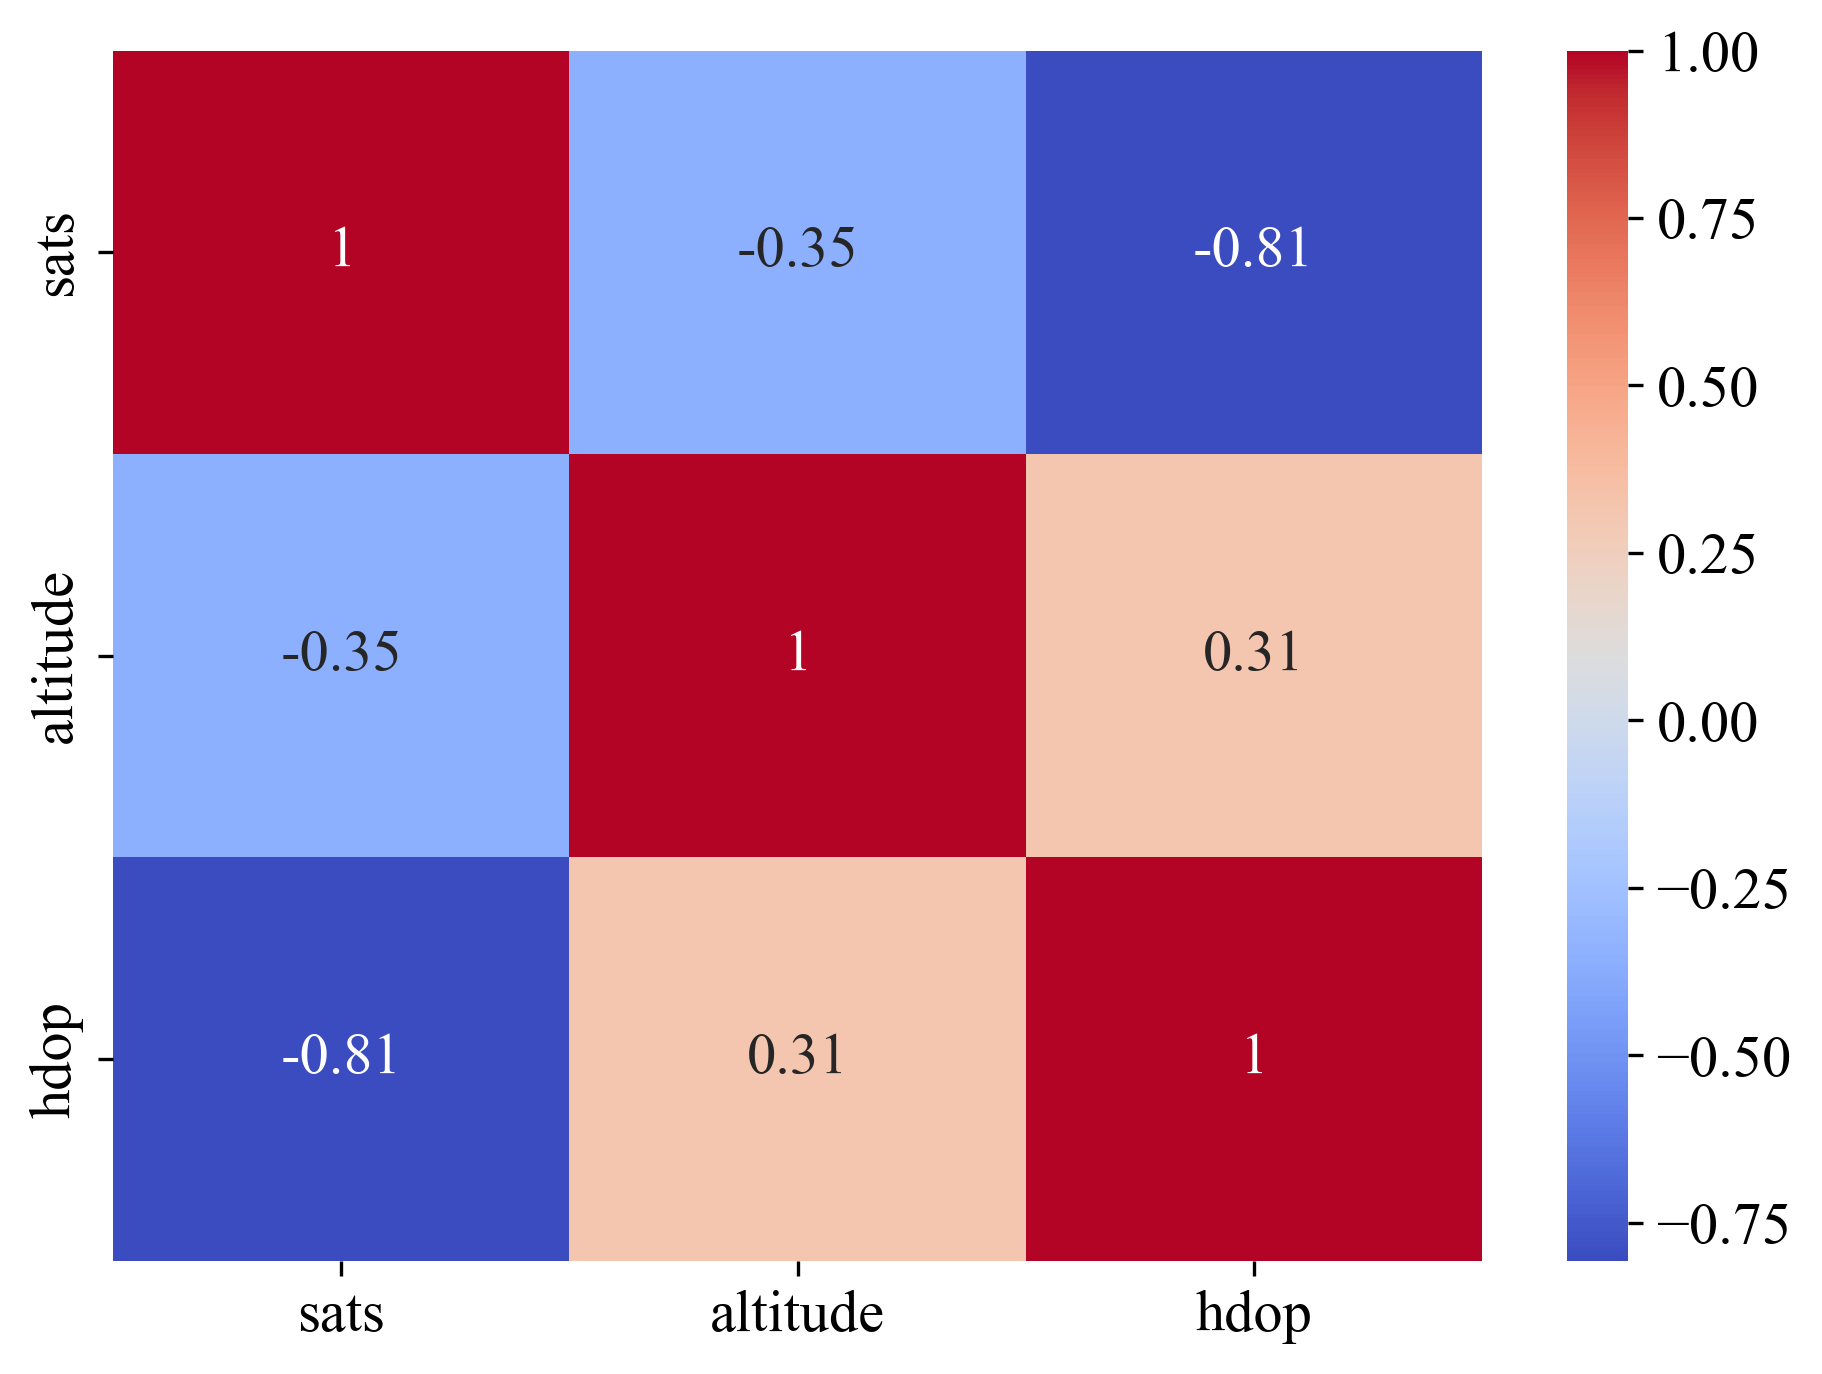
\includegraphics[width=11cm]{contents/chapter-4/pengujian-bergerak/corr.png}
	\caption{Korelasi setiap parameter pengujian di bus Trans Gadjah Mada}
	\label{Fig: moving-corr}
\end{figure}

Nilai korelasi dari lima parameter, yaitu visibilitas satelit, ketinggian, HDOP, VDOP dan PDOP ditunjukan oleh Gambar \ref{Fig: moving-corr}. Korelasi ketinggian dengan empat parameter lainnya menunjukan tingkat korelasi yang rendah sehingga parameter ketinggian tidak berdampak dengan hasil pengujian.  Visibilitas satelit dengan HDOP, VDOP, dan PDOP memiliki hubungan korelasi negatif. Korelasi visibilitas satelit dengan HDOP menunjukan korelasi yang kuat, sedangkan korelasi visibilitas satelit dengan dua nilai DOP lainnya menunjukan tingkat korelasi sedang. Hal tersebut menunjukan bahwa semakin banyak visibilitas satelit maka ketiga nilai DOP akan cenderung menurun. Terakhir, parameter PDOP dengan HDOP dan VDOP memiliki tingkat korelasi yang tinggi. Hal tersebut diakibatkan karena nilai PDOP adalah tingkat akurasi pada tiga dimensi sehingga nilai PDOP akan dipengaruhi oleh HDOP dan VDOP yang merupakan tingkat akurasi pada bidang horizontal dan vertikal.

Berdasarkan analisis korelasi di atas, parameter dengan korelasi paling tinggi adalah visibilitas satelit dengan ketiga nilai DOP dan antar ketiga nilai DOP. Oleh karena itu, pada bagian selanjutnya akan dibahas lebih lanjut mengenai HDOP, VDOP, PDOP, dan visibilitas satelit. 

\subsection{HDOP, VDOP, PDOP, dan Visibilitas Satelit}

Berdasarkan pembahasan pada bagian sebelumnya, pasangan variabel yang memiliki korelasi negatif adalah visibilitas satelit dengan HDOP, VDOP, dan PDOP dengan tingkat korelasi terhadap HDOP adalah tinggi, sedangkat untuk dua variabel lainnya tingkat korelasinya sedang. Di sisi lain, setiap pasangan variabel DOP memiliki korelasi positif yang kuat. Korelasi negatif menunjukan jika nilai dari salah satu variabel maka nilai dari variabel lainnya cenderung menurun dan hal sebaliknya untuk korelasi positif.

\begin{figure}[H]
	\centering
	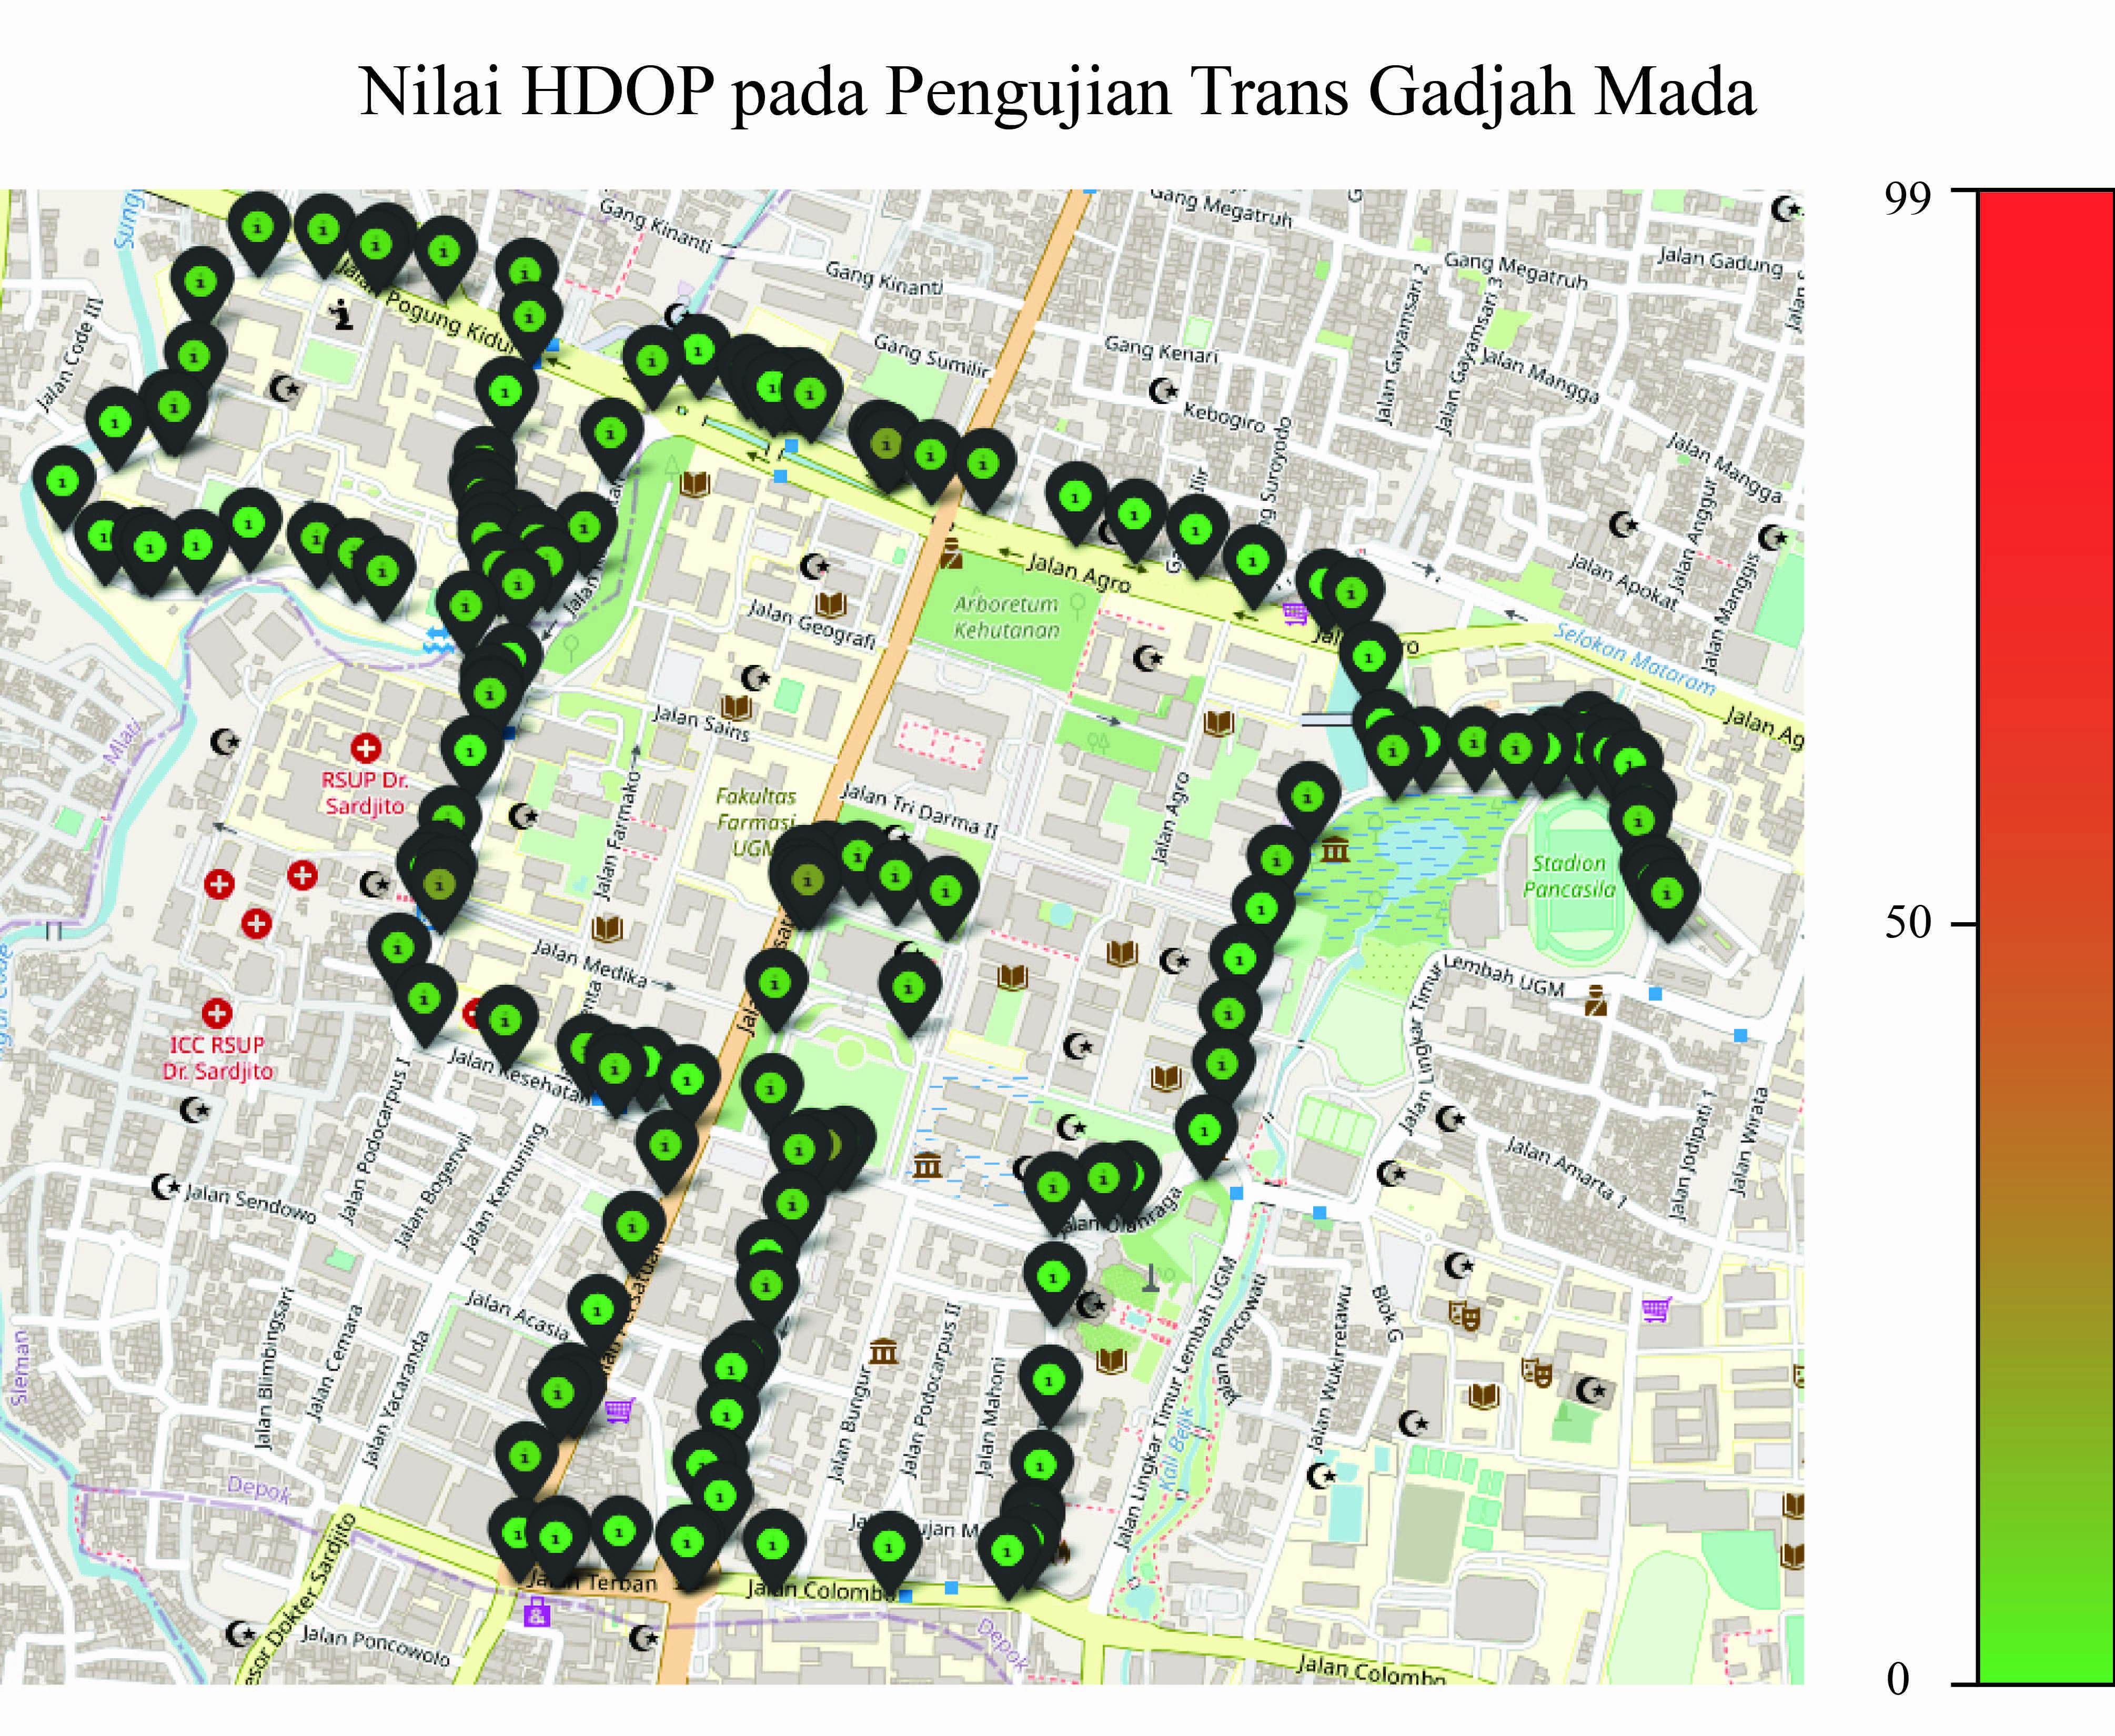
\includegraphics[width=12cm]{contents/chapter-4/pengujian-bergerak/moving-HDOP.jpg}
	\caption{Nilai HDOP pengujian di bus Trans Gadjah Mada rute 1B}
	\label{Fig: moving-hdop}
\end{figure}

Berdasarkan pembahasan pada bagian sebelumnya, dapat diketahui bahwa nilai HDOP yang rendah menunjukkan tingkat ketelitian yang lebih baik pada bidang horizontal. Hal ini dapat dilihat pada Gambar \ref{Fig: moving-hdop} dengan setiap titik pada perjalanan Trans Gadjah Mada rute 1B direpresentasikan dengan warna yang menunjukkan nilai HDOP pada titik tersebut. Semakin tinggi nilai HDOP, maka warna titiknya akan semakin mendekati warna merah, yang menunjukkan tingkat ketelitian yang lebih rendah. Sebaliknya, jika nilai HDOP semakin rendah, maka warna titiknya akan mendekati warna hijau, yang menunjukkan tingkat ketelitian yang lebih tinggi. Terlihat bahwa seluruh titik pada gambar tersebut direpresentasikan dengan warna hijau, yang menunjukkan bahwa tingkat akurasi pada bidang horizontalnya berada pada rentang yang baik.

\begin{figure}[H]
	\centering
	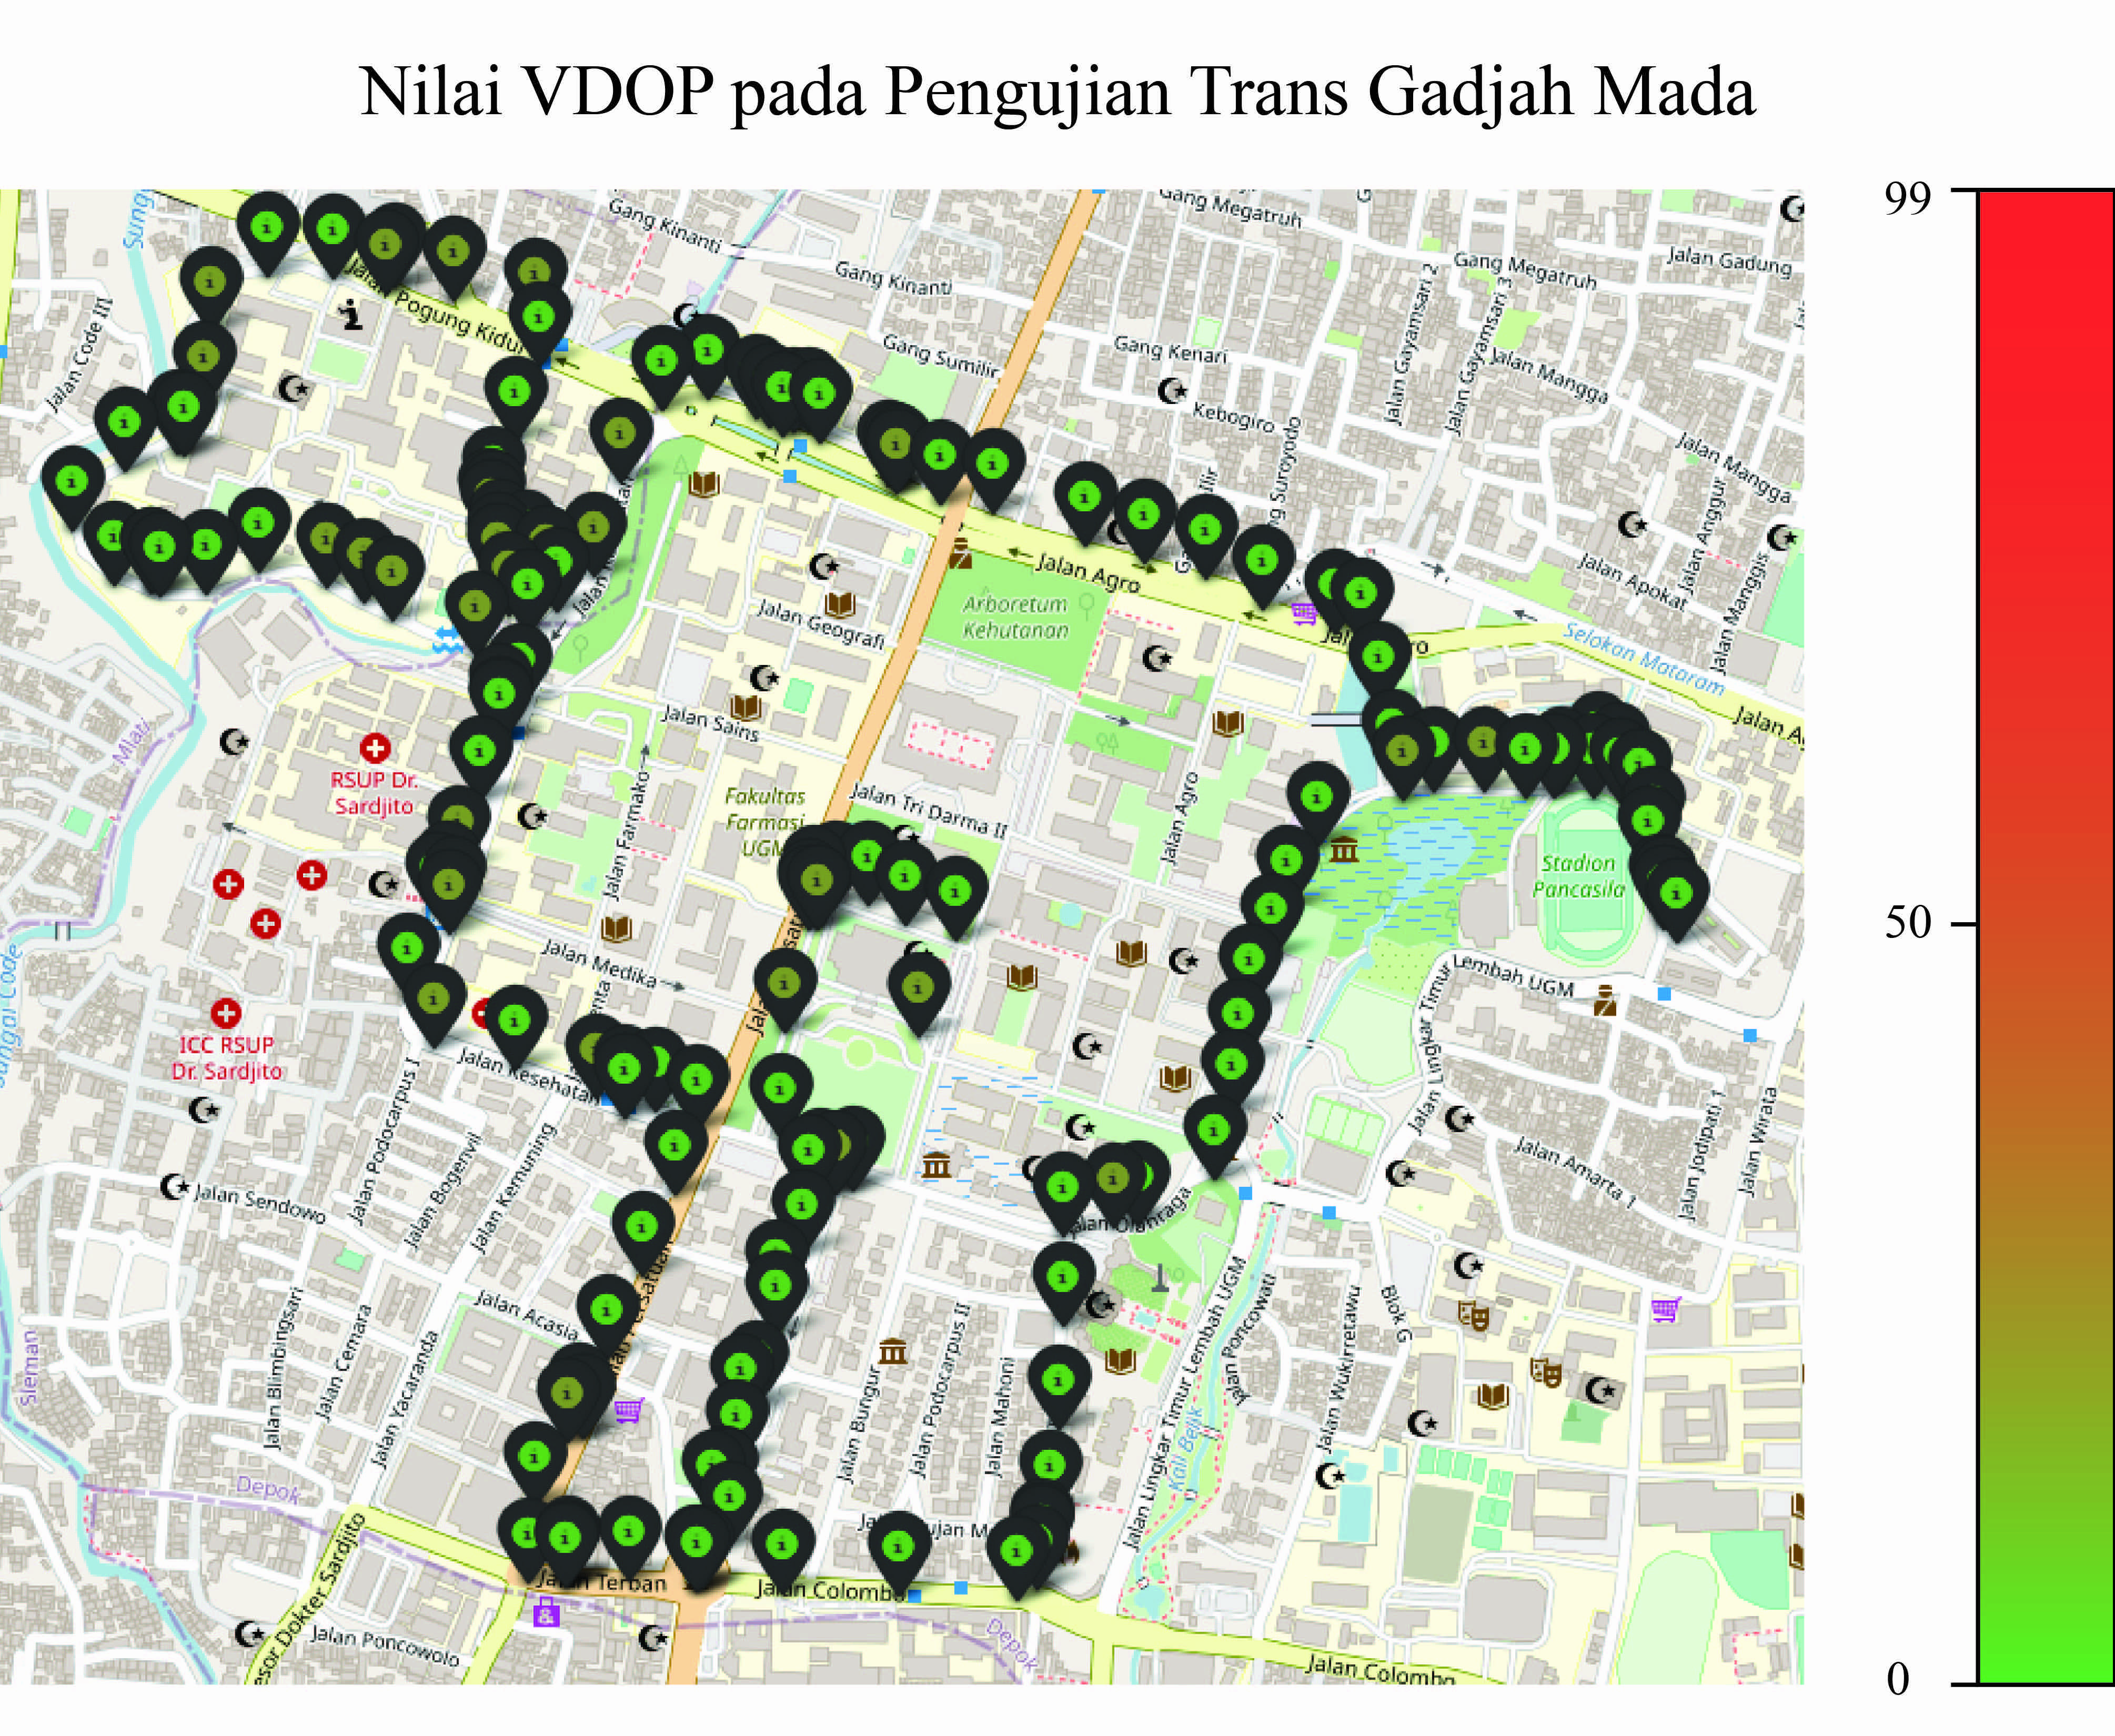
\includegraphics[width=12cm]{contents/chapter-4/pengujian-bergerak/moving-VDOP.jpg}
	\caption{Nilai VDOP pengujian di bus Trans Gadjah Mada rute 1B}
	\label{Fig: moving-vdop}
\end{figure}

Selain HDOP, parameter akurasi lain yang dapat ditinjau adalah VDOP. Parameter ini digunakan untuk mengukur tingkat akurasi pada bidang vertikal atau ketinggian. Nilai VDOP pada hasil pengujian dapat dilihat pada Gambar \ref{Fig: moving-pdop}. Semakin rendah nilai VDOP, maka titik pada gambar akan berwarna hijau. Dari gambar tersebut, terlihat bahwa seluruh titik pengamatan berwarna hijau, yang menandakan bahwa nilai VDOP-nya berada dalam rentang yang baik. Meskipun beberapa tempat tertutup oleh pepohonan atau banyak penghalang berupa gedung-gedung, akurasi sistem di bidang vertikal juga tidak terganggu secara signifikan. Oleh karena itu, dapat dilihat bahwa akurasi hasil pengukuran sistem pada bidang vertikal sudah sangat akurat.

\begin{figure}[H]
	\centering
	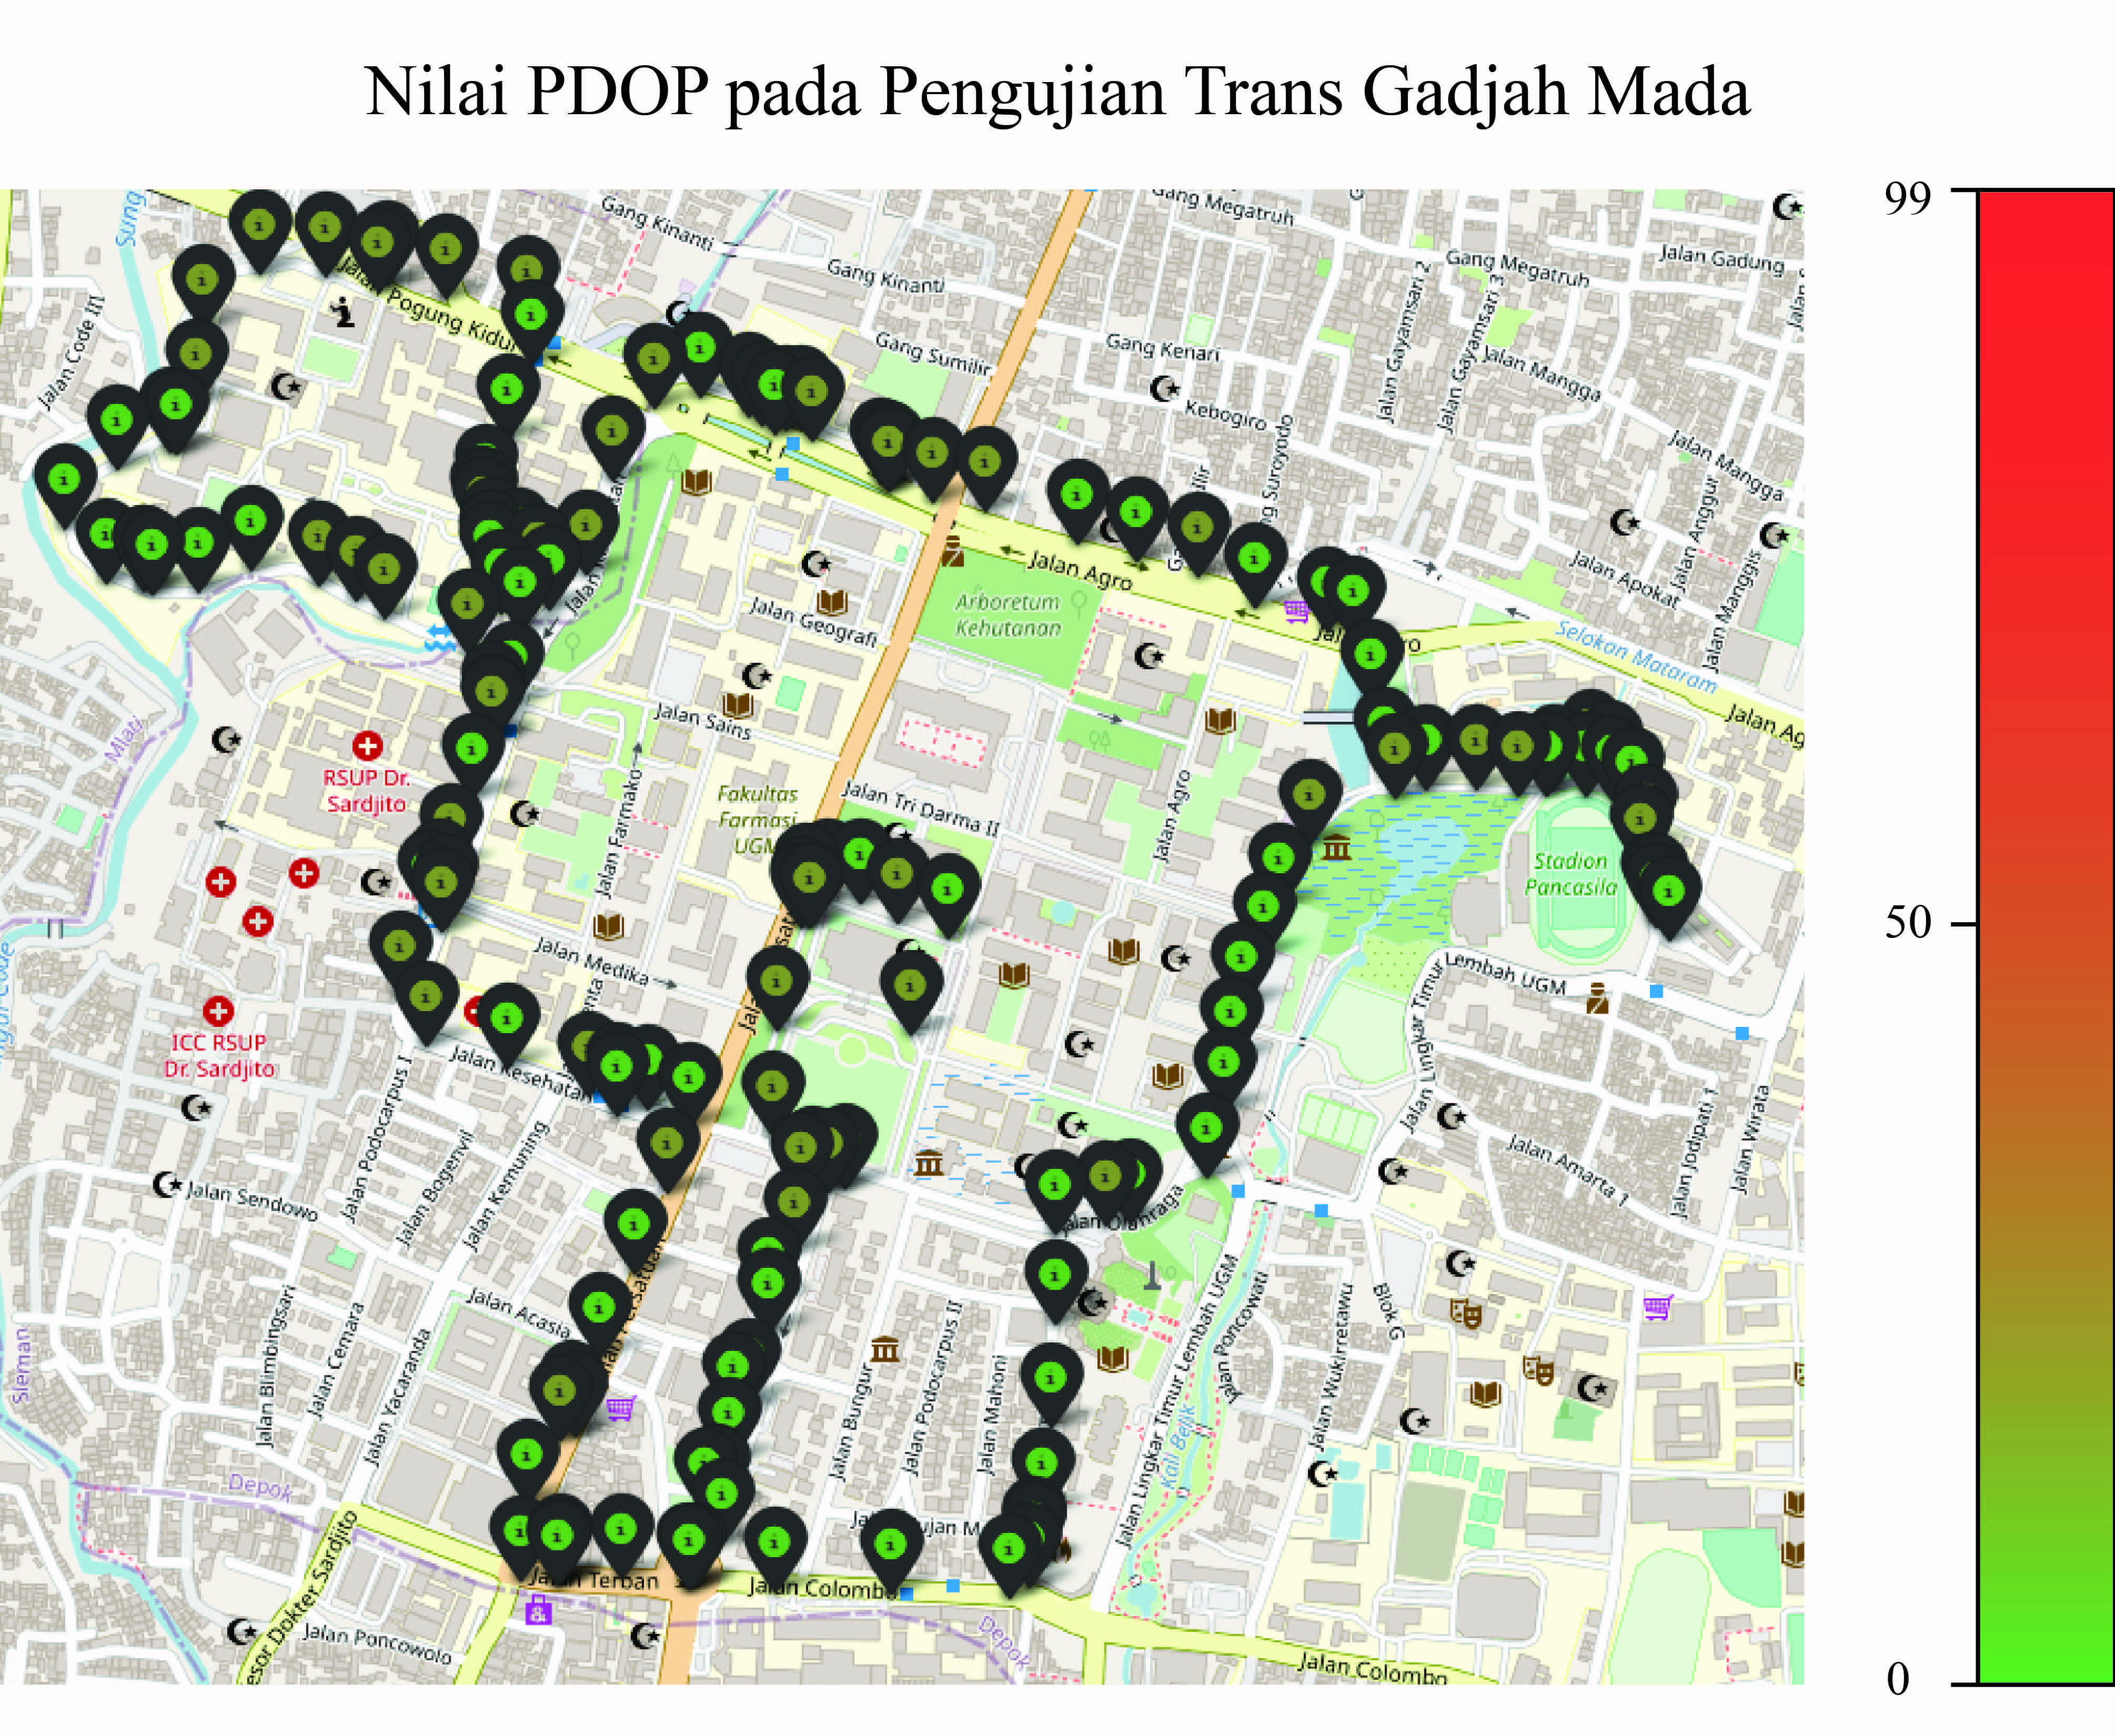
\includegraphics[width=12cm]{contents/chapter-4/pengujian-bergerak/moving-PDOP.jpg}
	\caption{Nilai PDOP pengujian di bus Trans Gadjah Mada rute 1B}
	\label{Fig: moving-pdop}
\end{figure}

Parameter PDOP merupakan gabungan dari HDOP dan VDOP. Artinya, nilai dari PDOP akan merepresentasikan tingkat akurasi hasil perhitungan baik di bidang horizontal maupun vertikal. Selain itu, nilai PDOP juga menjelaskan persebaran satelit di langit. Sama seperti dua nilai DOP lainnya, semakin rendah nilai PDOP maka semakin baik. Hasil pengamatan yang ditunjukan oleh Gambar \ref{Fig: moving-pdop} menunjukan bahwa nilai PDOP pada setiap titik pengamatan sudah sangat baik. Hal tersebut merupakah hasil yang sudah diharapkan karena PDOP adalah gabungan dari VDOP dan HDOP sehingga jika nilai HDOP dan VDOP sudah sangat baik maka nilai PDOP-nya juga akan sangat baik. Karena nilai PDOP juga bergantung pada geometri satelit, nilai tersebut juga menunjukan bahwa persebaran satelit di langit selama pengamatan sudah tersebar dengan sangat baik. 

\begin{figure}[H]
	\centering
	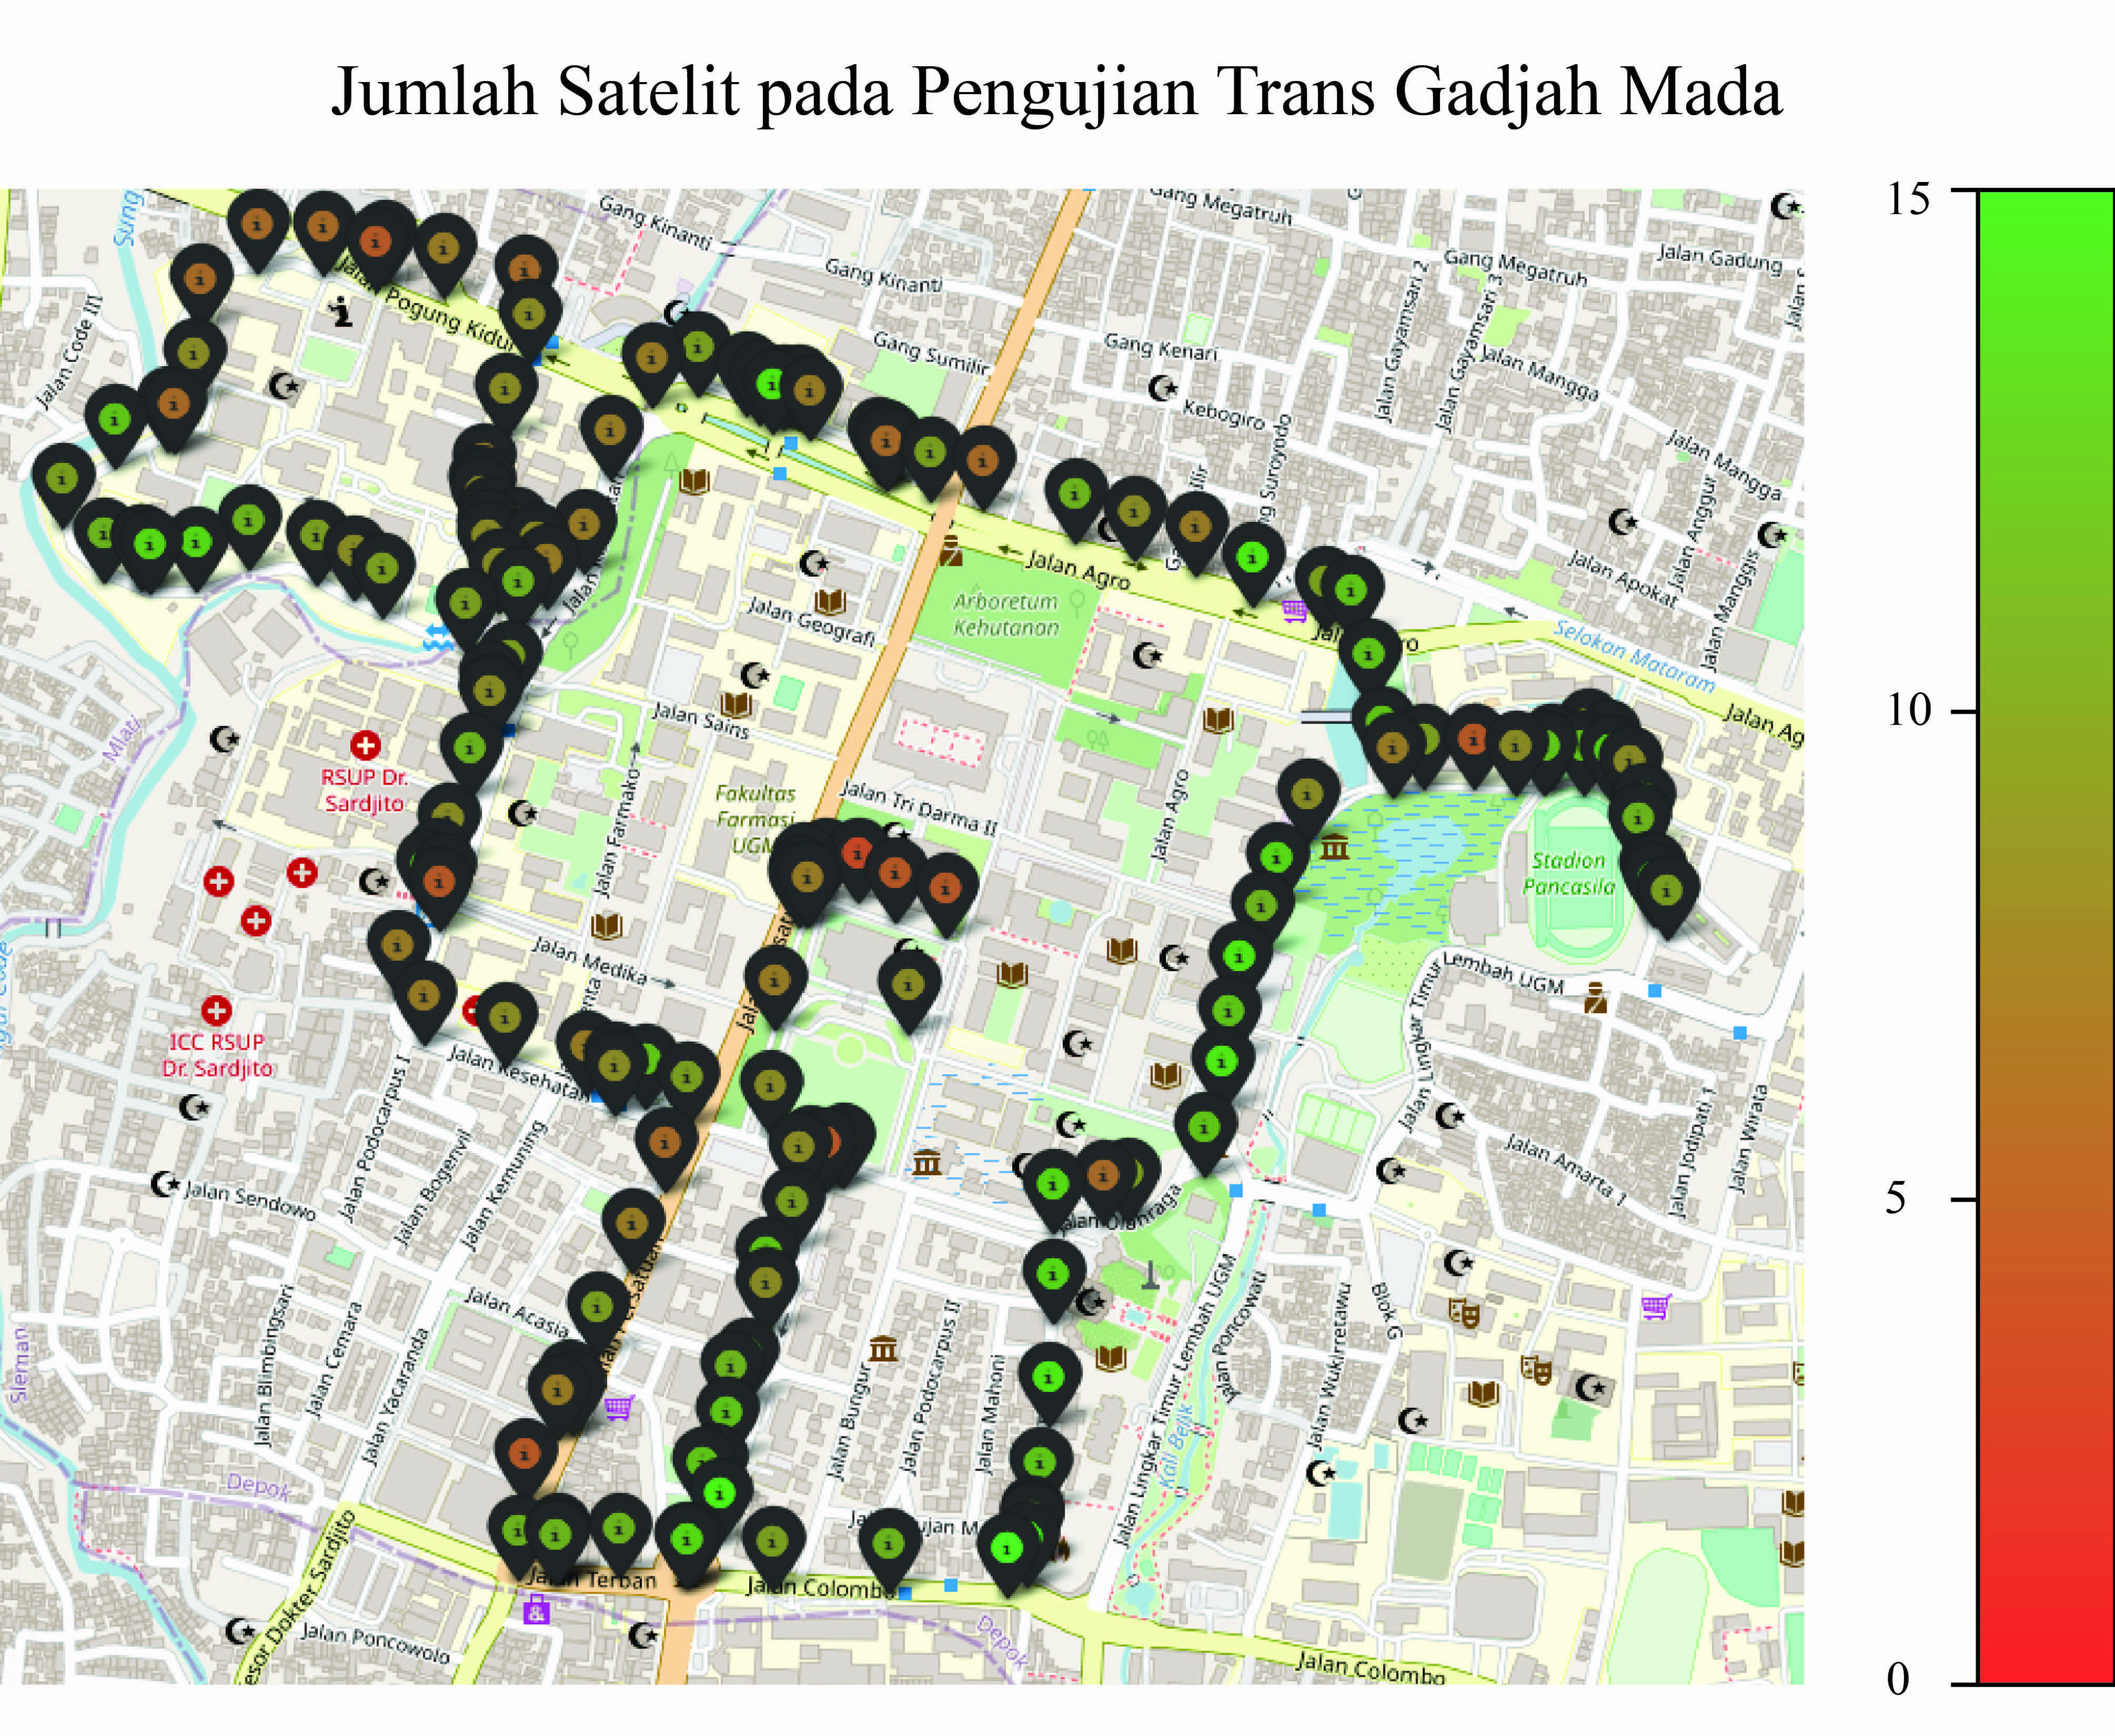
\includegraphics[width=12cm]{contents/chapter-4/pengujian-bergerak/moving-SATS.jpg}
	\caption{Visibilitas satelit pengujian di bus Trans Gadjah Mada rute 1B}
	\label{Fig: moving-sats}
\end{figure}

Visibilitas satelit adalah jumlah satelit yang digunakan untuk melakukan perhitungan posisi. Jumlah satelit yang digunakan tentunya akan mempengaruhi ketelitian hasil perhitungan posisi. Gambar \ref{Fig: moving-sats} menunjukan visibilitas satelit di setiap titik pada perjalanan Trans Gadjah Mada rute 1B. Semakin tinggi visibilitas satelit maka warna titiknya akan mendekati warna hijau dan mendekati warna merah jika visibilitas satelitnya mendekati nol. Secara teoretis, visibilitas satelit yang dibutuhkan untuk mendapatkan fiksasi 2D adalah sebanyak tiga buah dan empat buah untuk mendapatkan fiksasi 3D. Visibilitas satelit lebih dari empat akan memperbaiki kualitas fiksasi yang ditunjukan dengan nilai HDOP yang menurun. 

Pada hasil pengamatan dapat dilihat bahwa tidak semua titik memiliki visibilitas satelit lebih dari sepuluh atau direpresentasikan dengan titik berwarna hijau. Visibilitas satelit paling rendah pada pengujian ini adalah sebanyak enam buah satelit yang ditunjukan oleh titik berwarna merah. Salah satu titik dengan visibilitas terendah adalah di sekitar halte Rumah Sakit Dr. Sardjito. Hal tersebut dapat diakibatkan oleh banyaknya gedung dan pepohonan yang dapat menghalangi atau menyebabkan \textit{multipath} pada isyarat GNSS. Selain itu, lingkungan tersebut juga merupakan lingkungan yang padat dengan berbagai macam kendaraan dan orang-orang yang lalu-lalang.

Meskipun terdapat beberapa titik dengan visibilitas satelit sejumlah enam buah, nilai HDOP, VDOP, dan PDOP pada lokasi tersebut tetap berwarna hijau tua atau baik. Hal tersebut dikarenakan visibilitas satelit yang dimiliki sudah melebihi batas minimal visibilitas satelit untuk mendapat fiksasi 3D, yaitu empat buah satelit. Angka visibilitas satelit yang lebih banyak tentunya dapat menurunkan nilai DOP hingga mendekati nol seperti ditunjukan pada titik di depan Rumah Sakit Panti Rapih. Visibilitas satelit pada titik tersebut sebanyak tujuh belas buah dengan nilai HDOP 0,7; VDOP; 1,1; dan PDOP 1,2.